\begin{document}

\frontmatter

\thetitlepage
\cleardoublepage
\setcounter{page}{1}

\section{Abstract}
\uwabstract
\cleardoublepage

\section{Acknowledgements}
The content of this thesis reflects the work of a wide group of physicists collaborating on an analysis project and sharing their knowledge.  I received much guidance from Vuko Briglevi\'{c} and Tulika Bose while enjoying camaraderie in the trenches with Cory Fantasia, Sre\'{c}ko Morovi\'{c}, and Irakli Svintradze as they applied their ingenuity to make our measurements work.

My efforts have been greatly aided by the encouragement of my officemates Mike Anderson and Will Maier.  They stretched my concept of what computers can do and pushed me to tackle bolder problems than I would have attempted on my own.

Matt Herndon, serving as my graduate advisor, gave me the freedom to explore what inspired me while providing the support to understand complex details of our measurements and their significance.  In particular, this document is much stronger due to his careful reading and deeply thoughtful comments.

My family has been extremely supportive throughout my graduate work, including foremost my wife, Karen, and my parents, Arnie and Carol.

\clearpage

\maxtocdepth{subsection}
\tableofcontents\clearpage
\listoffigures\clearpage
\listoftables\clearpage

\mainmatter
\linenumbers

\chapter{Introduction}

Physics currently recognizes four fundamental forces which account for nearly all known phenomena in physics.  A handful of notable observations from the past few decades, however, have identified key deficiencies in our existing model.  Much of the basic research being conducted in physics today is focused on exploring modifications or additions to the known forces and matter particles in order to provide explanations for these new observations.

This thesis describes an experimental search for such new physics using the Compact Muon Solenoid (CMS), a four-story-high detector housed 300 feet underground designed to study particle interactions produced by the Large Hadron Collider (LHC).  The LHC is the highest-energy particle accelerator ever constructed and has brought together thousands of physicists from across the globe interested in pushing the frontiers of knowledge to ever-smaller scales.

We will start by considering an overview of the Standard Model of particle physics (Chapter~\ref{chapter:standard-model}), a theory which describes the fundamental forces as arising from the exchange of various mediating \emph{bosons} between particles of matter.  The more specific focus of the thesis on $W$ and $Z$ bosons, the mediators of the weak force, is discussed in Chapter~\ref{chapter:wz-theory} along with motivation for investigations into associated $WZ$ production as a probe to reveal new physics.  Previous experimental work which informs our current understanding of weak interactions is introduced in Chapter~\ref{chap:previous}, leading to an-depth explanation in Chapter~\ref{chapter:experiment} of the capabilities of the CMS detector and the LHC.

Chapters~\ref{chapter:simulation} through~\ref{chapter:background} discuss the various tools and strategies used in building a compelling analysis of particle collision data and in particular the method used to isolate and understand a sample of $WZ$ events recorded by CMS.  All of this builds to a presentation of two new investigations performed using this collision data.  First is a measurement of the $WZ$ cross section (Chapter~\ref{chapter:cross-section}) which is a generalized description of the frequency with which $WZ$ events are produced in a particular type of collision.  Measuring that interaction probability is an important demonstration of our analysis capabilities and provides a first window for probing deviations from the predictions of the Standard Model.  In Chapter~\ref{chapter:limits}, we move on to an explicit investigation of new physics by looking for an excess of $WZ$ events clustered around a mass value corresponding to a new heavy particle.  We provide new limits on the production of such a particle and discuss the constraints they provide on a variety of proposed models for new physics.

\section{Terminology and Conventions}

In many areas of physics which involve investigations at small scales, energies are discussed not in terms of the typical SI units of Joules, but rather in terms of the electron volt (\eV), equal to the fundamental unit of charge multiplied by the SI unit of electric potential.  Most energies discussed in this text will be in terms of $\GeV = \SI{e9}{\eV}$ or $\TeV = \SI{e12}{\eV}$.

Particle interactions at the \GeV or \TeV scale are necessarily relativistic, meaning that the energies associated with the particles' rest masses ($E_0 = mc^2$) are insignificant in comparison to their kinetic energies.  Relativistic velocities are characterized by the Lorentz factor:
\begin{equation}
  \gamma = \frac{1}{\sqrt{1 - \frac{v^2}{c^2}}},
\end{equation}
with $v$ the velocity of the particle and $c$ the speed of light in a vacuum.  The total energy of a particle is given by its rest energy and momentum as $E = \sqrt{E_0^2 + (pc)^2}$ and can be expressed in terms of the Lorentz factor as $E = \gamma mc^2$, meaning that the kinetic portion of the total energy is given by $T = (\gamma - 1)mc^2$.
Considering that an electron with kinetic energy of just \sienergy{1} achieves a Lorentz factor $\gamma \approx 2000$, this relation makes clear that the rest mass of most particles plays no significant role in the relativistic limit.  As a result, we often speak of a ``\SI{10}{\GeV} electron'' or a ``\TeV muon'' where the energy value refers interchangeably to the total energy or the kinetic energy.  Indeed, particle physicists routinely drop the factors of $c$ from their equations and speak of mass and momentum in energy units, understanding that others in the community can easily infer their intended meaning.  In an effort to remain accessible to a wider audience, this thesis  maintains the distinctions between energy, momentum, and mass, along with their associated units (\GeV, \GeVc, and \GeVcc) whenever possible.

The existence of antiparticles, one of the early discoveries of the particle physics era, has become an integral piece of the field theories which describe relativistic interactions.  While antiparticles share most characteristics including mass with their particle counterparts, other properties are inverted.  When discussion demands a distinction between particles and antiparticles, it is usually sufficient to specify the electric charges; thus, an electron is designated $e^-$ while the antielectron or \emph{positron} is designated $e^+$.  In the case of neutral particles or when specification of electric charge would be distracting, an alternate notation is used where antiparticles receive an overbar; we can then distinguish a neutrino $\nu$ from an antineutrino $\bar{\nu}$ or a proton $p$ from an antiproton $\bar{p}$.  Because antiparticles are quite common in high-energy interactions, the distinction between matter and antimatter is often ignored.  Unless explicitly stated otherwise, a reference to ``electrons'' refers also to positrons while a reference to ``muons'' apply equally to $\mu^+$ as it does to $\mu^-$.

Our theoretical understanding of particle interactions is deeply mathematical, enabling us to produce incredibly precise predictions for observable processes based on various quantum field theories.  While the calculations can be complex, they can be constructed in a rather straight-forward manner from simple \emph{Feynman diagrams} (example in Fig.~\ref{fig:example-feynman}) which show the possible interactions as pictures.  For this thesis, I will use the convention that the horizontal axis of the diagram represents time, so that particles on the left represent the initial state and particles on the right represent the final state.

\begin{figure}[h]
  \centering
  \begin{tikzpicture}[thin, level/.style = {level distance = 1.6cm, line width = 1pt} ]
  \coordinate 
  child[grow = 150] { 
    edge from parent [fermion, backwards] node [above = 2pt] {$q$} 
  }
  child[grow = -150] { 
    edge from parent [fermion, forwards] node [below = 2pt] {$q^\prime$} 
  }
  child[grow = east] { 
    child[grow = 30] {
      edge from parent [boson] node [above = 2pt] {$W$}}
    child[grow = -30] { 
      edge from parent [boson] node [below = 2pt] {$\gamma$}}
    edge from parent [boson] node [above = 0pt] {$W$}
  }
  ;
\end{tikzpicture}

  \caption{An example Feynman diagram.}
  \label{fig:example-feynman}
\end{figure}

Each line represents a particle, with solid lines for fermions and wavy lines for bosons.  The arrows on the fermion lines represent the particles' momenta, meaning that arrows pointing toward the left represent particles traveling \emph{backwards} in time.  This is the Feynman diagram convention for representing antiparticles, which are indeed physically equivalent to the corresponding matter particles running in reverse.  The convention makes it easy to turn or twist the diagram to represent related processes.  By assigning momenta to the various lines and coupling values to the various vertices where those lines come together, these diagrams can be translated directly into equations which predict the probability for a given interaction.

\chapter{Introduction}

Physics currently recognizes four fundamental forces which account for nearly all known phenomena in physics.  A handful of notable observations from the past few decades, however, have identified key deficiencies in our existing model.  Much of the basic research being conducted in physics today is focused on exploring modifications or additions to the known forces and matter particles in order to provide explanations for these new observations.

This thesis describes an experimental search for such new physics using the Compact Muon Solenoid (CMS), a four-story-high detector housed 300 feet underground designed to study particle interactions produced by the Large Hadron Collider (LHC).  The LHC is the highest-energy particle accelerator ever constructed and has brought together thousands of physicists from across the globe interested in pushing the frontiers of knowledge to ever-smaller scales.

We will start by considering an overview of the Standard Model of particle physics (Chapter~\ref{chapter:standard-model}), a theory which describes the fundamental forces as arising from the exchange of various mediating \emph{bosons} between particles of matter.  The more specific focus of the thesis on $W$ and $Z$ bosons, the mediators of the weak force, is discussed in Chapter~\ref{chapter:wz-theory} along with motivation for investigations into associated $WZ$ production as a probe to reveal new physics.  Previous experimental work which informs our current understanding of weak interactions is introduced in Chapter~\ref{chap:previous}, leading to an-depth explanation in Chapter~\ref{chapter:experiment} of the capabilities of the CMS detector and the LHC.

Chapters~\ref{chapter:simulation} through~\ref{chapter:background} discuss the various tools and strategies used in building a compelling analysis of particle collision data and in particular the method used to isolate and understand a sample of $WZ$ events recorded by CMS.  All of this builds to a presentation of two new investigations performed using this collision data.  First is a measurement of the $WZ$ cross section (Chapter~\ref{chapter:cross-section}) which is a generalized description of the frequency with which $WZ$ events are produced in a particular type of collision.  Measuring that interaction probability is an important demonstration of our analysis capabilities and provides a first window for probing deviations from the predictions of the Standard Model.  In Chapter~\ref{chapter:limits}, we move on to an explicit investigation of new physics by looking for an excess of $WZ$ events clustered around a mass value corresponding to a new heavy particle.  We provide new limits on the production of such a particle and discuss the constraints they provide on a variety of proposed models for new physics.

\section{Terminology and Conventions}

In many areas of physics which involve investigations at small scales, energies are discussed not in terms of the typical SI units of Joules, but rather in terms of the electron volt (\eV), equal to the fundamental unit of charge multiplied by the SI unit of electric potential.  Most energies discussed in this text will be in terms of $\GeV = \SI{e9}{\eV}$ or $\TeV = \SI{e12}{\eV}$.

Particle interactions at the \GeV or \TeV scale are necessarily relativistic, meaning that the energies associated with the particles' rest masses ($E_0 = mc^2$) are insignificant in comparison to their kinetic energies.  Relativistic velocities are characterized by the Lorentz factor:
\begin{equation}
  \gamma = \frac{1}{\sqrt{1 - \frac{v^2}{c^2}}},
\end{equation}
with $v$ the velocity of the particle and $c$ the speed of light in a vacuum.  The total energy of a particle is given by its rest energy and momentum as $E = \sqrt{E_0^2 + (pc)^2}$ and can be expressed in terms of the Lorentz factor as $E = \gamma mc^2$, meaning that the kinetic portion of the total energy is given by $T = (\gamma - 1)mc^2$.
Considering that an electron with kinetic energy of just \sienergy{1} achieves a Lorentz factor $\gamma \approx 2000$, this relation makes clear that the rest mass of most particles plays no significant role in the relativistic limit.  As a result, we often speak of a ``\SI{10}{\GeV} electron'' or a ``\TeV muon'' where the energy value refers interchangeably to the total energy or the kinetic energy.  Indeed, particle physicists routinely drop the factors of $c$ from their equations and speak of mass and momentum in energy units, understanding that others in the community can easily infer their intended meaning.  In an effort to remain accessible to a wider audience, this thesis  maintains the distinctions between energy, momentum, and mass, along with their associated units (\GeV, \GeVc, and \GeVcc) whenever possible.

The existence of antiparticles, one of the early discoveries of the particle physics era, has become an integral piece of the field theories which describe relativistic interactions.  While antiparticles share most characteristics including mass with their particle counterparts, other properties are inverted.  When discussion demands a distinction between particles and antiparticles, it is usually sufficient to specify the electric charges; thus, an electron is designated $e^-$ while the antielectron or \emph{positron} is designated $e^+$.  In the case of neutral particles or when specification of electric charge would be distracting, an alternate notation is used where antiparticles receive an overbar; we can then distinguish a neutrino $\nu$ from an antineutrino $\bar{\nu}$ or a proton $p$ from an antiproton $\bar{p}$.  Because antiparticles are quite common in high-energy interactions, the distinction between matter and antimatter is often ignored.  Unless explicitly stated otherwise, a reference to ``electrons'' refers also to positrons while a reference to ``muons'' apply equally to $\mu^+$ as it does to $\mu^-$.

Our theoretical understanding of particle interactions is deeply mathematical, enabling us to produce incredibly precise predictions for observable processes based on various quantum field theories.  While the calculations can be complex, they can be constructed in a rather straight-forward manner from simple \emph{Feynman diagrams} (example in Fig.~\ref{fig:example-feynman}) which show the possible interactions as pictures.  For this thesis, I will use the convention that the horizontal axis of the diagram represents time, so that particles on the left represent the initial state and particles on the right represent the final state.

\begin{figure}[h]
  \centering
  \begin{tikzpicture}[thin, level/.style = {level distance = 1.6cm, line width = 1pt} ]
  \coordinate 
  child[grow = 150] { 
    edge from parent [fermion, backwards] node [above = 2pt] {$q$} 
  }
  child[grow = -150] { 
    edge from parent [fermion, forwards] node [below = 2pt] {$q^\prime$} 
  }
  child[grow = east] { 
    child[grow = 30] {
      edge from parent [boson] node [above = 2pt] {$W$}}
    child[grow = -30] { 
      edge from parent [boson] node [below = 2pt] {$\gamma$}}
    edge from parent [boson] node [above = 0pt] {$W$}
  }
  ;
\end{tikzpicture}

  \caption{An example Feynman diagram.}
  \label{fig:example-feynman}
\end{figure}

Each line represents a particle, with solid lines for fermions and wavy lines for bosons.  The arrows on the fermion lines represent the particles' momenta, meaning that arrows pointing toward the left represent particles traveling \emph{backwards} in time.  This is the Feynman diagram convention for representing antiparticles, which are indeed physically equivalent to the corresponding matter particles running in reverse.  The convention makes it easy to turn or twist the diagram to represent related processes.  By assigning momenta to the various lines and coupling values to the various vertices where those lines come together, these diagrams can be translated directly into equations which predict the probability for a given interaction.

% \chapter{The Standard Model}
\label{chapter:standard-model}


\section{History and Overview}

The Standard Model of particle physics combines into one theory all the major successes of the past century concerning our theoretical understanding of fundamental particles and their interactions.  It incorporates three of the four known fundamental forces (electromagnetism, the weak nuclear force, and the strong nuclear force), leaving only gravity out of the picture.  In 1960, Sheldon Glashow succeeded in unifying electromagnetic and weak interactions into a single electroweak theory~\cite{Weinberg:1967tq}, later working concurrently with Steven Weinberg and Abdus Salam to explain the weak boson masses by incorporating the Higgs mechanism~\cite{PhysRevLett.13.508,PhysRevLett.13.321,PhysRevLett.13.585}.  By the mid-seventies, the modern theory of the strong interaction was also completed.  In the decades since, the Standard Model has been strikingly successful as new experiments have verified Standard Model predictions to ever-increasing accuracy.

The Standard Model rests on the concept of quantized energy and momentum relations, forming a set of quantum field theories associated with the fundamental forces.  The properties of the forces are reflected in the symmetries of their respective field theories.  In the language of group theory, the Standard Model can be described as:
\begin{equation}
  SU(3)_C \times SU(2)_\text{L} \times U(1)_Y,
\end{equation}
with the $SU(3)_C$ group corresponding to the strong force generated by color charge $C$, the $SU(2)_\text{L}$ group corresponding to weak isospin $T_3$ (relevant only for left-handed particles), and the $U(1)$ group corresponding to weak hypercharge $Y$.  Each group implies a gauge symmetry which enforces conservation of the associated charge and determines the properties of the resulting gauge bosons which mediate the interaction.  The $SU(2)_\text{L} \times U(1)_Y$ piece describes the mixing and unification of the weak and electromagnetic forces in Glashow's original electroweak theory.  Of particular interest is the non-Abelian nature of this symmetry which gives rise to weak bosons which themselves carry weak charge.  As a result, it becomes possible to have direct interactions between these bosons, with significant implications which will be discussed in Chapter~\ref{chapter:wz-theory}.


\section{Fundamental Particles}
The particle content of the Standard Model is naturally split into \emph{fermions} which constitute matter and \emph{bosons} which carry forces.  The fermions can be further divided into two distinct families --- the \emph{quarks} which interact via the strong nuclear force and the \emph{leptons} which do not (Table~\ref{tab:fermions}).  Among the bosons, the electromagnetic force is mediated by the photon~($\gamma$), the weak force is mediated by the $W$ and the~$Z$, and the strong force is mediated by gluons~($g$) (Table~\ref{tab:bosons}).

\newcommand{\masshead}{\ensuremath{mc^2 / \eV}}

\begin{table*}
  \centering
  \newcommand{\mysep}{$\:\times$ 10}
  \begin{tabular}{r r r r l r@{\mysep}l l r@{\mysep}l l r@{\mysep}l}
    \toprule
    & & & & \multicolumn{3}{c}{$1^\text{st}$ Generation} & \multicolumn{3}{c}{$2^\text{nd}$ Generation} & \multicolumn{3}{c}{$3^\text{rd}$ Generation} \\ 
    \cmidrule(r){4-6} \cmidrule(rl){7-9} \cmidrule(l){10-12}
    $s$ & $Q$ & $T_3$ & $C$ & $f$ &  \multicolumn{2}{c}{\masshead} & $f$ & \multicolumn{2}{c}{\masshead} & $f$ & \multicolumn{2}{c}{\masshead} \\
    \midrule
    $\frac{1}{2}$ & $+\frac{2}{3}$ & $+\frac{1}{2}$ & 1 & $u$ & 3&$^6$ & $c$ & 1.27&$^9$ & $t$ & 1.72&$^{11}$ \\
    $\frac{1}{2}$ & $-\frac{1}{3}$ & $-\frac{1}{2}$ & 1 & $d$ & 5&$^6$ & $s$ & 1.01&$^8$ & $b$ & 4.67&$^9$\\
    $\frac{1}{2}$ & $0$ & $+\frac{1}{2}$ & 0 & $\nu_e$ & < 2.2&$^{0}$ & $\nu_\mu$ & < 1.7&$^{5}$ & $\nu_\tau$ & < 1.55&$^{7}$ \\
    $\frac{1}{2}$ & $-1$ & $-\frac{1}{2}$ & 0 & $e$ & 5.11&$^{5}$ & $\mu$ & 1.06&$^8$ & $\tau$ & 1.78&$^9$ \\
    \bottomrule
  \end{tabular}
  \caption[Properties of the fundamental fermions]{The fundamental fermions, with spin $s$, electric charge $Q$, weak isospin $T_3$ (equal to zero for right-handed particles), presence or absence of color indicated by $C$ (the charge of the strong force, with quarks carrying one unit of red, green, or blue color), and mass $m$.  The common symbol used for each fermion is given by $f$, with up-type quarks in the first row, down-type quarks in the second, neutral leptons (neutrinos) in the third, and charged leptons in the fourth.  For each listed particle, there is a corresponding antiparticle with the same mass, but opposite values of $Q$ and $T_3$.}
  \label{tab:fermions}
\end{table*}

\begin{table*}
  \centering
  \newcommand{\mysep}{$\:\times$ 10}
  \begin{tabular}{c c r r r r c}
    \toprule
    Symbol & Interaction & $s$ & $Q$ & $T_3$ & C & \masshead \\
    \midrule
    $\gamma$ & electromagnetism & 1 & 0 & 0 & 0 &0 \\
    $W$ & weak nuclear force    & 1 & $\pm$ 1 & $\pm$ 1 & 0 & \phantom{>} \num{8.04e10} \\
    $Z$ & weak nuclear force    & 1 &       0 &       0 & 0 & \phantom{>} \num{9.12e10} \\
    $g$ & strong nuclear force  & 1 &       0 &       0 & 1 & 0 \\
    $H$ & ---                   & 0 & 0 & 0 & 0 & > \num{1.15e11}\\
    \bottomrule
  \end{tabular}
  \caption[Properties of the fundamental bosons]{The fundamental bosons with spin $s$, electric charge $Q$, weak isospin $T_3$ (the charge of the $SU(2)$ interaction), presence or absence of color indicated by $C$ (the charge of the strong force, with all bosons colorless except for the bicolored gluon), and mass $m$.}
  \label{tab:bosons}
\end{table*}

The normal matter of everyday life is made up of just three fundamental fermions.  The protons and neutrons that form the nucleus of any atom are each colorless clusters of three quarks, tightly bound together via the strong force.  The proton consists of two up quarks and a down quark ($uud$) while the neutron has one up and two down ($udd$).  No atom would be complete, however, without electrons~($e^{-}$) orbiting the nucleus to balance the positive electric charge of the protons.  Together with the electron neutrino~($\nu_e$, a nearly massless particle which interacts very rarely), these form the first generation of matter particles.  

While the additional two fermion generations (the charm, strange, top, and bottom quarks along with the muon and tau, and their associated neutrinos) are otherwise identical to the first, they carry substantially greater masses.  Due to couplings with the $W$ boson, these heavy fermions are able to participate in interactions which cross generational boundaries and are thus unstable.  They can exist only momentarily before they decay, leaving behind first generation fermions.  Experimental evidence confirms that only these three generations exist~\cite{:2005ema}, but a theoretical explanation for that number is one of the unanswered questions of the Standard Model (discussed further in Sec.~\ref{sec:shortcomings}).

\section{Fundamental Particles in the Context of a Collider}
While the Standard Model provides a pleasantly polished roster of distinct particles, most of these are highly unstable and thus rarely found in nature.  We must use colliders to produce bursts of energy intense enough to produce them, then view the lower mass products into which they decay.  As such, we now take a more pragmatic look at how fundamental particles behave in that context.

The structure of the strong interaction ensures asymptotic freedom~\cite{PhysRevLett.30.1343}, meaning that the strength of the interaction becomes arbitrarily weak only at small separations between quarks; the strength of the interaction actually grows as colored particles move apart.  As a result, quarks simply cannot survive outside the confines of a colorless hadron.  A high-momentum quark immediately begins shedding its energy by pulling $q\bar{q}$ pairs out of the vacuum, thereby providing new partners with which to form colorless bound states.  An experimentalist sees the result of this \emph{hadronization} process as a collimated \emph{jet} of charged and neutral particles.  The total energy of a jet, which is closely related to that of the original quark, can be determined by measuring the momenta of the charged hadrons as they bend in a magnetic field along with the total energy deposited by the charged and neutral particles as they interact with a dense material.  These strong and electromagnetic interactions produce showers of secondary particles which can be directly detected, as described below.  Of the six quark flavors, the notable exception to this rule of hadronization is the extremely massive top quark whose lifetime is too short to form bound states; it instead decays directly to the lighter fermions.

Among the charged leptons, only the electron is truly stable, although its low mass makes it prone to \brem when passing through matter, a process of energy emission in the form of photons which can further split to form new electron-positron pairs.  Assuming a high momentum for the original electron, this splitting is likely to continue several times over, forming a cascade known as an electromagnetic shower.  Despite the splitting, the energy of a primary electron can be determined with high accuracy by measuring the total energy released in the shower.

Surprisingly, the unstable muon often turns out to be a cleaner object for experimental observation than the stable electron, as its high mass suppresses \brem losses.  At \GeV energy scales, its relatively long lifetime (\SI{2.2}{\micro s}) allows a muon to travel through hundreds of meters of matter before decaying to an electron.  The muon, then, can be directly detected by sampling its trajectory as it moves through a magnetic field.

In contrast to the electron and muon, the tau lepton decays much too quickly to be identified directly in a detector.  Reconstruction of a tau relies on piecing together its decay products, which will be some combination of electrons, muons, and jets.

The neutral leptons (\emph{neutrinos}) are the most elusive of the fundamental particles.  They are light enough to be stable and they interact only via the weak force, giving them the unique ability to pass through large quantities of matter undisturbed.  Experiments which detect neutrinos are able to sample only a small fraction of the neutrinos passing through their detectors, so they rely on dedicated sources with large statistics to mitigate the low interaction probability.  In the context of a collider, an individual neutrino is entirely untraceable.  When searching for processes involving a neutrino, the collider experimentalist's only recourse is to employ conservation laws, knowing that no particle in the initial state has a momentum component transverse to the beampipe.  By analyzing the distribution of energy deposits for all detectable particles, we can detect an imbalance in the transverse direction (\MET) to associate with a supposed neutrino (a more detailed description of this technique is given in Sec.~\ref{sec:met}).

Each of the bosons can be observed using some combination of the techniques already discussed.  Photons are stable and can be detected by the same electromagnetic showers seen for electrons.  Gluons ejected from collisions hadronize similarly to the quarks, so they can also be observed through jets of charged particles.  The $W$ and $Z$ bosons may decay through a variety of channels, producing either leptons or hadrons.

\section{Electroweak Symmetry Breaking}

Mathematically, the electromagnetic and weak nuclear forces are nearly identical, suggesting a strong symmetry.  Each can be described by a potential:
\begin{equation}
  V \approx \frac{1}{r}e^{-mr},
\end{equation}
with $r$ the distance between two interacting particles and $m$ the mass of the boson mediating the interaction.  Within quantum field theory, the interaction is described as a set of probabilities proportional to:
\begin{equation}
  \frac{g^4}{(q^2c^2 - m^2c^4)^2},
\end{equation}
with $m$ as before, $q$ the momentum transferred between the interacting particles, and $g$ the coupling associated with the force.  The electromagnetic and weak couplings are intimately related, with $g_\text{EM} = -e$ and $g_\text{weak} = -e \cot{\theta_\text{W}}$ differing only by a multiplicative constant near unity ($\cot(\theta_\text{W}) \approx 1.7$) defined by the Weinberg or ``weak mixing'' angle $\theta_\text{W}$.  The substantial low-energy asymmetry between the weak and electromagnetic forces, then, is not due to the coupling but rather due to the high mass of the $W$ and $Z$ bosons which limits the range of weak interactions in comparison to electromagnetic interactions mediated by the massless photon.

The coupling ``constant'' for an interaction is only an approximation, as its value actually depends on the momentum transfer involved in an interaction.  In contexts where this variation in energy scale becomes a noticeable effect, we speak of a ``running'' coupling constant.  In practice, however, we are indeed able to treat the electromagnetic and weak couplings as constant since the low-energy value of order \num{e-2} increases by only 10\% at the energy scale of $W$ and $Z$ bosons.  At energies much higher than those achievable with current colliders, quantum electrodynamics (QED) predicts that the running of the electromagnetic coupling does eventually become significant, yielding infinite contributions at finite energies which threaten to spoil the theory.  This divergence, though, is generally accepted as an indication that the theory is only a low-energy approximation of some more general interaction, so the true behavior of the coupling at high energy is unknown.  In contrast, the running of the strong force coupling is most pronounced at low energies, so calculations in the theory of quantum chromodynamics (QCD) must always be performed in reference to a particular energy scale.

At high energies ($q/c >> m$), the mass of the mediating boson no longer plays a significant role.  The values of the weak and electromagnetic couplings also converge in this region, leading the two interactions to have comparable strength and thus realizing the unification which is the hallmark of electroweak theory.  Understanding the symmetry within the theory, we now turn our attention to how an element can be introduced which breaks that symmetry in order to accomodate the observed behavior at low energy.

Within the Standard Model, electroweak symmetry breaking is effected through the Higgs mechanism which introduces a Higgs field $\varphi$ which generates mass-like terms in the Lagrangian~\cite{PhysRevLett.13.508,PhysRevLett.13.321,PhysRevLett.13.585}.  The Higgs field is a doublet in the $SU(2)$ electroweak interaction, but a singlet in the $SU(3)$ color interaction,
\begin{equation}
  \varphi = \left(\begin{array}{c}\varphi^+ \\ \varphi^0\end{array}\right).
\end{equation}

This field carries a potential,
\begin{equation}
  V(\varphi) = \mu^2\varphi^\dagger\varphi + \lambda(\varphi^\dagger\varphi)^2,
\end{equation}
with mass parameter $\mu^2$ and Higgs field self-interaction strength $\lambda$.  A positive or null value of $\mu^2$ would mean no Higgs interaction whatsoever; to provide an opportunity for the desired spontaneous symmetry breaking, we choose $\mu^2 < 0$, leading to a potential with degenerate minima,
\begin{equation}
  \varphi^\dagger\varphi = -\frac{\mu^2}{2\lambda} = \frac{v^2}{2},
\end{equation}
with $v=\sqrt{-\mu^2/\lambda}$ the vacuum expectation value of~$\varphi$.

\begin{figure}
\centering
\includegraphics[clip=true,trim=0.3in 0 0 0]{matplotlib/higgs.pdf}
\caption[The Higgs potential]{A qualitative plot of the Higgs potential ($V(\varphi)$), showing the ``champagne bottle'' shape.  There is no single minimum, but rather a circle of degenerate minima along the base of the bottle.}
\label{higgs-potential}
\end{figure}

This non-zero value for~$\varphi$ allows for interactions of massless free particles with the Higgs field at all points in space, making them appear massive.  In particular, the Standard Model Lagrangian includes terms quadratic in the fields for the vector bosons, leading to masses given by:
\begin{align}
  M(W) &= \frac{v|g|}{2}, \\
  M(Z) &= \frac{v\sqrt{g^2 + g^{\prime 2}}}{2}.
\end{align}
with $g$ and $g^\prime$ the couplings associated with $SU(2)$ and $U(1)$ gauge groups respectively.  At this point, we have achieved the electroweak symmetry breaking which was the original intention of the Higgs mechanism, although the theory can be extended to generate masses for the fermions as well.  If we choose to re-express the theory in terms of the field:
\begin{equation}
  \tilde{\varphi} = \varphi - \varphi_0,
\end{equation}
with $\varphi_0$ the Higgs field, we end up with ``Yukawa interaction'' terms $g\varphi_0\bar{\psi}\psi$ which correspond to a fermion with mass $g\varphi_0$.  At present, we have no theoretical motivation for the values of these Yukawa couplings $g$, leading to another set of parameters which must be experimentally derived.

While this is the simplest proposed mechanism for imparting mass to the Standard Model particles, we have yet to observe a Higgs boson, and discovering a Higgs is indeed one of the major physics goals of the LHC.  

\section{Shortcomings of the Standard Model}
\label{sec:shortcomings}

While the proposed Higgs mechanism in the Standard Model provides a comparatively simple explanation for electroweak symmetry breaking, it leaves open a variety of theoretical questions.  In particular, this elementary Higgs model \cite{Lane:2000pa,Shrock:2007km}
\begin{itemize}
\item provides no \emph{dynamical} explanation for electroweak symmetry breaking in the sense that the vacuum expectation value of the Higgs must be experimentally derived ($\mu^2$ could just as well be positive or zero, spoiling the theory),
\item seems \emph{unnatural} since it requires an enormously precise fine-tuning of parameters to avoid quadratically divergent contributions to the Higgs mass,
\item cannot explain the \emph{hierarchy problem} of a vast gap between the electroweak scale ($\mathcal{O}(\sienergy{e2})$) at which the Higgs gives mass to the weak bosons and the Planck scale ($\mathcal{O}(\sienergy{e19})$) at which gravity is expected to have a similar strength the SM forces,
\item is \emph{trivial} in that it is understood to be invalid beyond some cutoff scale $\Lambda$, and
\item provides no insight into \emph{flavor physics}, giving no explanation for fermion generations, masses, or mixing.
\end{itemize}

The triviality problem refers to the same behavior already discussed in quantum electrodynamics which predicts divergent contributions at high energy.  The problem is so named because the only way to avoid the divergent catastrophe without adding new elements to the theory is to require that the normalized charge be zero, leading to a ``trivial'' theory of noninteracting particles.  This characteristic is not generally seen as a problem in QED since the energy scale at which the theory becomes inconsistent is inaccessibly large, suggesting that the theory is a successful low-energy approximation of some more fundamental set of interactions.  The luxury of ignoring divergences, however, cannot be indulged for the Higgs mechanism as the predicted cut-off scale is much lower, perhaps within the energy reach of the LHC.

Several of these issues (particularly unnaturalness and the hierarchy problem) can be mitigated in supersymmetric models~\cite{Lane:2000pa}; indeed, LHC Higgs searches typically consider various supersymmetric configurations alongside the SM Higgs.  This thesis does not consider supersymmetry, but does consider various Higgless models (see Section~\ref{sec:technicolor}) which can also overcome these difficulties.

The success of Glashow's electroweak theory in unifying the electromagnetic and weak forces seems to suggest that all the fundamental forces may really be different aspects of one unified force, but the SM fails to fully integrate the strong force with the electroweak interaction and ignores gravity completely.  All efforts thus far to develop a quantum theory of gravity have failed, as quantum models seem incompatible with general relativity.  For the strong force, there is more hope, and a variety of so-called Grand Unified Theories have been proposed to fold color in with the electroweak interaction (see section \ref{sec:wprime}).

Other problems with the SM involve its limited scope.  While the SM has provided some tremendously accurate predictions, it relies on an unreasonable number of \emph{ad hoc} parameters which must be experimentally derived, including all the particle masses and couplings.  Besides this, the past few decades have produced several astronomical observations inconsistent with the existing content of the model.  In some regions of space where gravitational effects indicate matter should be present, we observe none of the radiation expected from the known massive particles, prompting speculation on new neutrino-like \emph{dark matter} candidates with no electromagnetic or strong couplings, but with mass great enough to explain the observed gravitational effects.  We have also observed an overall outward acceleration of the universe incompatible with any known force; the most promising explanations for this are \emph{dark energy} models where some new quantum field acquires a vacuum expectation value, but we have little to guide as at this point as to the details of such a theory.  Finally, the Standard Model fails to provide any mechanism which could explain the substantial dominance of matter over antimatter in the universe; while several experiments have confirmed some deviation in the behavior of matter vs.\ antimatter with respect to weak interactions, the small magnitude of the effect fails to provide any compelling explanation for the complete absence of bulk antimatter.

% Why a fundamental unit of charge?
% not enough CP violation

\resetlinenumber
\chapter{A Theoretical View of~Diboson~Production}
\label{chapter:wz-theory}

\section{Electroweak Diboson Production}

While all electroweak interactions involve at least one of the bosons $\gamma$, $W$, or $Z$, we can gain new insight into the structure of electroweak theory by considering interactions involving multiple electroweak bosons.  These interactions occur less frequently than single-boson events, but they lie within reach for modern colliders.  Indeed, all triple-boson couplings predicted to occur within the SM have already been observed (see discussion in Chapter~\ref{chap:previous}).

In order to participate in a given interaction, a particle must have a non-zero coupling to the associated boson, corresponding to a non-zero charge.  Table~\ref{tab:bosons}, describing the properties of the various gauge bosons, lists a non-zero value of weak isospin $T_3$ (corresponding to the $SU(2)$ interaction) only for the $W$ while the weak hypercharge $Y = 2(Q - T_3)$ associated with the $U(1)$ interaction is null for all gauge bosons.  As a result, the only couplings allowed in the SM directly between the various electroweak bosons is through the weak isospin of the $W$ which connects it to both the photon and the $Z$.  Thus, we expect to see $WWZ$ and $WW\gamma$ vertices, but never $ZZZ$, $ZZ\gamma$, $Z\gamma\gamma$, or $\gamma\gamma\gamma$; other conceivable combinations are forbidden because they would not conserve electric charge.

The values of the various charges ascribed to the electroweak bosons can be understood in terms of the gauge structure of the two interactions involved.  The observed neutral bosons $Z$ and $\gamma$ are in fact superpositions of the neutral $SU(2)$ boson $W^0$ and the $U(1)$ boson $B$.  Terms in the Lagrangian corresponding to multi-boson interactions arise from non-zero commutation relations within the corresponding group.  Because operators from different groups commute and because each operator necessarily commutes with itself, we cannot build any non-zero term involving only $W^0$ and $B$ operators.  The $WWZ$ and $WW\gamma$ interactions arise from terms which invoke the non-zero commutation relations between $W^0$ and $W^\pm$.

The simplest diagrams leading to diboson production can be drawn through simple reconfiguration of the familiar vertices which couple the gauge bosons to fermion pairs; at a hadron collider, this takes the form of two quarks individually radiating gauge bosons in the same event (Fig.~\ref{fig:dibosons-radiation}).  
%Because it carries an electric charge, the $W$ boson can also interact directly with the photon.  Furthermore, the non-Abelian nature of the weak interaction means that the weak bosons themselves carry weak charge and can interact directly.  This leads to the trilinear gauge couplings (TGCs) $WW\gamma$ and $WWZ$ as well as the quadrilinear gauge couplings (QGCs) .   
The annihilation of fermions to a single gauge boson with subsequent radiation of an additional boson (Fig.~\ref{fig:dibosons-annihilation}) involves the previously mentioned trilinear couplings while additional quartic couplings (QGCs) $W^+W^-W^+W^-$, $W^+W^-Z^0Z^0$, $W^+W^-\gamma^0\gamma^0$, and $W^+W^-Z^0\gamma^0$ come into play in diboson scattering events (Fig.~\ref{fig:dibosons-quartic}).  Finally, the SM predicts diagrams involving a Higgs boson which can decay to gauge boson pairs (Fig.~\ref{fig:dibosons-higgs}).

\begin{figure}
  \centering
  \begin{tikzpicture}[thin, level/.style = {level distance = 1.6cm, line width = 1pt} ]
  \coordinate 
  child[grow = 200] { 
    edge from parent [fermion, backwards] node [below = 2pt] {$q$}
  }
  child[grow = north, level distance = 1.0cm] { 
    child[grow = 160] {
      edge from parent [fermion, forwards] node [above = 2pt] {$q$}}
    child[grow = 30] { 
      edge from parent [boson] node [above = 2pt] {$\gamma$}}
    edge from parent [fermion, forwards] node [left = 0pt] {$q$}
  }
  child[grow = -30] {
    edge from parent [boson] node [below = 2pt] {$\gamma$}
  }
  ;
\end{tikzpicture}

  \hspace{1in}
  \begin{tikzpicture}[thin, level/.style = {level distance = 1.6cm, line width = 1pt} ]
  \coordinate 
  child[grow = 200] { 
    edge from parent [fermion, backwards] node [below = 2pt] {$q$}
  }
  child[grow = north, level distance = 1.0cm] { 
    child[grow = 160] {
      edge from parent [fermion, forwards] node [above = 2pt] {$q$}}
    child[grow = 30] { 
      edge from parent [boson] node [above = 2pt] {$W$}}
    edge from parent [fermion, forwards] node [left = 0pt] {$q^\prime$}
  }
  child[grow = -30] {
    edge from parent [boson] node [below = 2pt] {$W$}
  }
  ;
\end{tikzpicture}

  \caption{Example diagrams of diboson production through radiation from quarks.}
  \label{fig:dibosons-radiation}
\end{figure}

\begin{figure}
  \centering
  \begin{tikzpicture}[thin, level/.style = {level distance = 1.6cm, line width = 1pt} ]
  \coordinate 
  child[grow = 150] { 
    edge from parent [fermion, backwards] node [above = 2pt] {$q$} 
  }
  child[grow = -150] { 
    edge from parent [fermion, forwards] node [below = 2pt] {$q^\prime$} 
  }
  child[grow = east] { 
    child[grow = 30] {
      edge from parent [boson] node [above = 2pt] {$W$}}
    child[grow = -30] { 
      edge from parent [boson] node [below = 2pt] {$\gamma$}}
    edge from parent [boson] node [above = 0pt] {$W$}
  }
  ;
\end{tikzpicture}

  \caption{Example diagram of diboson scattering through quark annihilation.}
  \label{fig:dibosons-annihilation}
\end{figure}

\begin{figure}
  \centering
  \begin{tikzpicture}[thin, level/.style = {level distance = 1.6cm, line width = 1pt} ]
  \coordinate 
  child[grow = 200] { 
    edge from parent [fermion, backwards] node [below = 2pt] {$q$}
  }
  child[grow = north] { 
    child[grow = 160] {
      edge from parent [fermion, forwards] node [above = 2pt] {$q$}
    }
    child[grow = -30] { 
      child[grow = 30] {
        edge from parent [boson] node [above = 2pt] {$W$}}
      edge from parent [boson] node [above = 2pt] {$W$}
    }
    edge from parent [fermion, forwards] node [left = 0pt] {$q^\prime$}
  }
  child[grow = 30] {
    child[grow = -30] {
      edge from parent [boson] node [below = 2pt] {$W$}}
    edge from parent [boson] node [below = 2pt] {$W$}
  }
  ;
\end{tikzpicture}  

  \caption{Example diagram of diboson scattering involving a quartic gauge coupling.}
  \label{fig:dibosons-quartic}
\end{figure}

\begin{figure}
  \centering
  \begin{tikzpicture}[thin, level/.style = {level distance = 1.6cm, line width = 1pt} ]
  \coordinate 
  child[grow = west] { 
    % bottom incoming quark
    edge from parent [fermion, backwards] node [below = 2pt] {$q$}
  }
  child[grow = 30] { 
    child[grow = 150] {
      child[grow = west] {
        % top incoming quark
        edge from parent [fermion, forwards] node [above = 2pt] {$q$}
      }
      child[grow = 30] {
        edge from parent [fermion, backwards] node [left=2pt, above=0pt] {$q^\prime$}
      }
      edge from parent [boson] node [above=4pt, right=0pt] {$W$}
    }
    child[grow = east] {
      child[grow = 30] {
        edge from parent [boson] node [left = 2pt, above = 2pt] {$W$}
      }
      child[grow = -30] {
        edge from parent [boson] node [left = 2pt, below = 2pt] {$W$}
      }
      edge from parent [fermion, forwards] node [below = 0pt] {$H$}
    }
    edge from parent [boson] node [below=4pt, right=0pt] {$W$}
  }
  child[grow = -30] {
    edge from parent [fermion, forwards] node [left = 2pt, below=0pt] {$q^\prime$}
  }
  ;
\end{tikzpicture}  

  \caption{Example diagram of diboson production involving a Higgs boson.}
  \label{fig:dibosons-higgs}
\end{figure}

Each diagram given in Figs.~\ref{fig:dibosons-radiation} through~\ref{fig:dibosons-higgs} shows the simplest configuration which leads to that interaction.  Experimental measurements, however, cannot discriminate between these diagrams and more complex ones which yield the same final state.  In general, the contribution from a given diagram decreases rapidly as the number of vertices increases, since each vertex introduces a suppression to the interaction probability on the order of the coupling value, meaning that higher order diagrams can be ignored.  The same is not necessarily true in the case of QCD interactions where the coupling can be of order unity.  We are fortunate that at the energy scale of weak bosons, the coupling is small enough that a ``perturbative QCD''~cite{Ellis1979285} approach which considers only some finite set of the simplest diagrams can provide the needed precision.  It becomes useful then to talk about the maximum ``order'' in the QCD coupling $\alpha_\text{s}$ considered for a given calculation.  The simplest diagrams are ``leading order'' while those involving one or two extra factors of $\alpha_\text{s}$ are ``next-to-leading'' (NLO) or ``next-to-next-to-leading'' (NNLO).

\section{Associated $WZ$ Production}

\begin{figure*}
  \center
  \newcommand{\spacer}{\hspace{0.5in}}
  \subbottom{
    \begin{tikzpicture}[thin, level/.style = {level distance = 2.0cm, line width = 1pt} ]
      \coordinate 
      child[grow =  90] {edge from parent [boson] node [right = 0pt] {$Z$}}
      child[grow = 210] {edge from parent [boson] node [above = 1pt] {$W$}}
      child[grow = 330] {edge from parent [boson] node [above = 1pt] {$W$}}
      ;
    \end{tikzpicture}
  }
  \spacer
  \subbottom{
    \begin{tikzpicture}[thin, level/.style = {level distance = 2.0cm, line width = 1pt} ]
      \coordinate 
      child[grow =  45] {edge from parent [boson] node [right = 4pt] {$W$}}
      child[grow = 135] {edge from parent [boson] node [left  = 4pt] {$W$}}
      child[grow = 225] {edge from parent [boson] node [left  = 4pt] {$W$}}
      child[grow = 315] {edge from parent [boson] node [right = 4pt] {$W$}}
      ;
    \end{tikzpicture}
  }
  \spacer
  \subbottom{
    \begin{tikzpicture}[thin, level/.style = {level distance = 2.0cm, line width = 1pt} ]
      \coordinate 
      child[grow =  45] {edge from parent [boson] node [right = 4pt] {$Z$}}
      child[grow = 135] {edge from parent [boson] node [left  = 4pt] {$W$}}
      child[grow = 225] {edge from parent [boson] node [left  = 4pt] {$W$}}
      child[grow = 315] {edge from parent [boson] node [right = 4pt] {$Z$}}
      ;
    \end{tikzpicture}
  }
\caption{The three vertices giving direct couplings between the weak bosons.}
\label{fig:tgc-vertices}
\end{figure*}

The particular focus of this thesis is on events where $W$ and $Z$ bosons are produced in association from the same hard-scattering interaction.  Within the SM, there are two QGCs and one TGC which involve both the $W$ and the $Z$ (Fig.~\ref{fig:tgc-vertices}).  The two leading order diagrams (given in Fig.~\ref{fig:wz-diagrams}) which contribute to $WZ$ production at the LHC are the $t$-channel process whereby a quark and antiquark emit $W$ and $Z$ bosons through exchange of a quark propagator and the $s$-channel process in which two quarks annihilate to an off-shell $W$ with subsequent radiation of a $Z$ boson.  There exist many possibilities for the subsequent decays of the vector bosons (Fig.~\ref{pie-decays}), but the cleanest experimental signatures come from their leptonic decays.

\begin{figure*}[!htbp]
  \centering
  \subbottom[$s$-channel]{
    \label{fig:wz-schannel}
    \begin{tikzpicture}[thin, level/.style = {level distance = 1.6cm, line width = 1pt} ]
  \coordinate 
  child[grow = 150] { 
    edge from parent [fermion, backwards] node [above = 2pt] {$q$} 
  }
  child[grow = -150] { 
    edge from parent [fermion, forwards] node [below = 2pt] {$q^\prime$} 
  }
  child[grow = east] { 
    child[grow = 30] {
      child[grow = 15] {
        edge from parent [fermion, forwards] node [above = 0pt] {$\ell$}}
      child[grow = -15] {
        edge from parent [fermion, backwards] node [below = 0pt] {$\nu_\ell$}}
      edge from parent [boson] node [above = 2pt] {$W$}}
    child[grow = -30] { 
      child[grow = 15] {
        edge from parent [fermion, forwards] node [above = 0pt] {$\ell^\prime$}}
      child[grow = -15] {
        edge from parent [fermion, backwards] node [below = 0pt] {$\ell^\prime$}}
      edge from parent [boson] node [below = 2pt] {$Z$}}
    edge from parent [boson] node [above = 0pt] {$W$}
  }
  ;
\end{tikzpicture}

  }
  \hspace{0.8in}
  \subbottom[$t$-channel]{
    \label{fig:wz-tchannel}
    \begin{tikzpicture}[thin, level/.style = {level distance = 1.6cm, line width = 1pt} ]
  \coordinate 
  child[grow = 200] { 
    edge from parent [fermion, backwards] node [below = 2pt] {$q$}
  }
  child[grow = north, level distance = 1.0cm] { 
    child[grow = 160] {
      edge from parent [fermion, forwards] node [above = 2pt] {$q^\prime$}}
    child[grow = 30] { 
      child[grow = 15] {
        edge from parent [fermion, forwards] node [above = 0pt] {$\ell$}}
      child[grow = -15] {
        edge from parent [fermion, backwards] node [below = 0pt] {$\nu_\ell$}}
      edge from parent [boson] node [above = 2pt] {$W$}}
    edge from parent [fermion, forwards] node [left = 0pt] {$q$}
  }
  child[grow = -30] {
    child[grow = 15] {
      edge from parent [fermion, forwards] node [above = 0pt] {$\ell^\prime$}}
    child[grow = -15] {
      edge from parent [fermion, backwards] node [below = 0pt] {$\ell^\prime$}}
    edge from parent [boson] node [below = 2pt] {$Z$}
  }
  ;
\end{tikzpicture}

  }\phantom{\hspace{0.2in}}
  \\
  \subbottom[quartic scattering]{
    \label{fig:wz-scattering}
    \begin{tikzpicture}[thin, level/.style = {level distance = 1.6cm, line width = 1pt} ]
  \coordinate 
  child[grow = west] {
    % bottom-left quark
    edge from parent [fermion, backwards] node [below = 2pt] {$q$}
  }
  child[grow = north] { 
    child[grow = west] {
      % top-left quark
      edge from parent [fermion, forwards] node [above = 2pt] {$q^\prime$}
    }
    child[grow = -30] { 
      child[grow = 30] {
        child[grow = 15] {
          edge from parent [fermion, forwards] node [above = 0pt] {$\ell$}
        }
        child[grow = -15] {
          edge from parent [fermion, backwards] node [below = 0pt] {$\nu_\ell$}
        }
        edge from parent [boson] node [above = 2pt] {$W$}
      }
      edge from parent [boson] node [above = 2pt] {$W$}
    }
    edge from parent [fermion, forwards] node [left = 0pt] {$q$}
  }
  child[grow = 30] {
    child[grow = -30] {
      child[grow = 15] {
        edge from parent [fermion, forwards] node [above = 0pt] {$\ell^\prime$}
      }
      child[grow = -15] {
        edge from parent [fermion, backwards] node [below = 0pt] {$\ell^\prime$}
      }
      edge from parent [boson] node [below = 2pt] {$Z$}
    }
    edge from parent [boson] node [below = 2pt] {$Z$}
  }
  ;
\end{tikzpicture}
    
  }
  \hspace{0.5in}
  \subbottom[Higgs-mediated scattering]{
    \label{fig:wz-scattering-higgs}
    \begin{tikzpicture}[thin, level/.style = {level distance = 1.6cm, line width = 1pt} ]
  \coordinate 
  child[grow = west] {% bottom-left quark from qqZ vertex
    edge from parent [fermion, backwards] node [below = 2pt] {$q$}
  }
  child[grow = 30] {% initial Z
    child[grow = north, level distance = 0.7cm] {% Higgs
      child[grow = 150] {% initial W
        child[grow = west] {% top-left incoming quark
          edge from parent [fermion, forwards] node [above = 2pt] {$q^\prime$}
        }
        child[grow = 30] {% top-left incoming quark
          edge from parent [fermion, forwards] node [above = 2pt] {$q$}
        }
        edge from parent [boson] node [above = 5pt, right = 0] {$W$}
      }
      child[grow = 30] {% final W
        child[grow = 15] {
          edge from parent [fermion, forwards] node [above = 0pt] {$\ell$}
        }
        child[grow = -15] {
          edge from parent [fermion, backwards] node [below = 0pt] {$\nu_\ell$}
        }
        edge from parent [boson] node [above = 5pt, left = 0] {$W$}
      }
      edge from parent [fermion] node [right = 0pt] {$H$}
    }
    child[grow = -30] {% final Z
      child[grow = 15] {
        edge from parent [fermion, forwards] node [above = 0pt] {$\ell^\prime$}
      }
      child[grow = -15] {
        edge from parent [fermion, backwards] node [below = 0pt] {$\ell^\prime$}
      }
      edge from parent [boson] node [below = 5pt, left = 0] {$Z$}
    }
    edge from parent [boson] node [below = 5pt, right = 0] {$Z$}
  }
  child[grow = -30] {
    edge from parent [fermion, forwards] node [below = 2pt] {$q$}
  }
  ;
\end{tikzpicture}

  }
  \caption[Diagrams for $WZ$ production]{Major production modes contributing to the $WZ$ states under study.  The leading order $s$-channel and $t$-channel processes dominate.  The quartic scattering diagram, by itself divergent, is balanced in the SM by interference from the Higgs-mediated scattering diagram.  The final-state leptons $\ell$ and~$\ell^{\prime}$ may be either electrons or muons.}
  \label{fig:wz-diagrams}
\end{figure*}

Although much more rare, processes that involve the scattering of longitudinally polarized gauge bosons can also result in the production of $WZ$ pairs (Fig.~\ref{fig:wz-scattering}).  These are particularly interesting because the amplitudes for such scattering processes violate unitarity at the \TeV scale in the absence of an interfering process to suppress the contribution~\cite{Han:2009em}.  The simplest scenarios which can provide such a process involve either a SM Higgs (Fig.~\ref{fig:wz-scattering-higgs}) or some new particle with similar characteristics.  Direct observation of these scattering processes is within the reach of the LHC, but the required collision statistics (on the order of \SI{100}{\fbinv}) for an observation will likely not be available for several years.  Alternative mechanisms for breaking the electroweak symmetry, however, could lead to enhancements which would make this process observable more quickly.  Thus, measurements of associated $WZ$ production provide tantalizing insights into the structure of the electroweak theory regardless of outcome; disagreement with Standard Model predictions would indicate new physics while agreement provides further evidence for the existence of a Higgs particle providing the needed interference.

The Standard Model Lagrangian contains the following terms to describe the $WWZ$ coupling:
\begin{equation}
  \label{eq:sm-tgc-lagrangian}
  \mathcal{L}_{WWZ}^\text{SM} = -i g_{WWZ}\, \left[(W_{\mu\nu}^\dag W^\mu - W^{\mu\dag}W_{\mu\nu})\, Z^\nu + W_\mu^\dag W_\nu\, Z^{\mu\nu} \,\right],
\end{equation}
with $W_\mu$ denoting the $W$ field, $W_{\mu\nu} = \partial W_\nu - \partial W_\mu$, $Z_\mu$ denoting the $Z$ field, $Z_{\mu\nu} = \partial Z_\nu - \partial Z_\mu$, and coupling $g_{WWZ} = -e \cot{\theta_\text{W}}$.  New physics could add extra terms which augment the SM contribution to this vertex.  Such anomalous TGCs provide a model-independent language with which to discuss constraints on physics beyond the Standard Model parameterized in terms of an \emph{effective} Lagrangian~\cite{Hagiwara:1986vm,doi:10.1146/annurev-nucl-102010-130106}:
\begin{align}
  \mathcal{L}_{WWZ}^\text{eff} = -i g_{WWZ}\; \Big[\;
  & g_1^Z\, (W_{\mu\nu}^\dag W^\mu - W^{\mu\dag}W_{\mu\nu})\, Z^\nu + \nonumber\\
  & k_Z\, W_\mu^\dag\, W_\nu\; Z^{\mu\nu} + \\
  & \frac{\lambda_Z}{M_W^2}\, W_\mu^{\nu\dagger}\, W_\nu^\rho\; Z_\rho^\mu\; \Big],\nonumber
\end{align}
which reduces to $\mathcal{L}_{WWZ}^\text{SM}$ by setting $g_1^Z = k_Z = 1$ and $\lambda_Z = 0$.  Searches for new physics through anomalous gauge couplings typically present their results as limits on the deviation of these parameters from their SM values.

%TODO: what specific changes would be expected for different models under consideration?

In a particle experiment, we are often interested in predicting and measuring the rate at which different types of interactions occur.  The observed event rate ($dN/dt$) is highly dependent on the particular configuration of the experiment at any given moment, so we tend to express it as a \emph{cross section} ($\sigma$) which describes the likelihood of the interaction multiplied by a \emph{luminosity} ($\mathcal{L}$) which describes the intensity of the beam,
\begin{equation}
  \label{eq:cross-section}
  \frac{dN}{dt} = \sigma\mathcal{L}.
\end{equation}
The cross section depends only on the energy of the collider, so it serves as a convenient characterization of the probability of a given process occurring.

By integrating Eq.~\ref{eq:cross-section} with respect to some period of collision activity, we obtain an \emph{integrated luminosity}:
\begin{equation}
  L = \int_{t_0}^{t} \mathcal{L}\,dt = \frac{N}{\sigma},
\end{equation}
for the number of produced events $N$ for a process with cross section $\sigma$ over a period $\Delta t = t - t_0$.  The integrated luminosity is a convenient measure of the quantity of collision data produced in an experiment since it has dimensions of inverse cross section, typically expressed in \pbinv or $\fbinv = \SI{1000}{\pbinv}$.  For a process with $\sigma = \SI{10}{pb}$, for example, we would expect on average one event for every \SI{0.1}{\pbinv} of integrated luminosity.

Conceptually, the cross section for a process is analogous to the area presented by a target to a stream of incoming projectiles, but it takes into account that particle interactions are described by probabilities rather than hits and misses.  One goal of this thesis will be to measure the cross section for $WZ$ production at the LHC (Chapter~\ref{chapter:cross-section}).

For LHC operation at $\sqrt{s} = \SI{7}{\TeV}$, we expect~\cite{Campbell:2011bn}
\begin{equation}
  \label{eq:predicted-cross-section}
  \sigma_\text{NLO}(p + p \to W^\pm + Z) = 18.57 \pm 0.95\,\si{pb}
\end{equation}
based on the most up-to-date theoretical predictions.  This next-to-leading order (NLO) calculation takes into account spin correlations as well as corrections for the probability of radiating an additional jet, but the calculated value is still dominated by contributions from the leading order $s$-channel and $t$-channel diagrams.  These calculations must rely on measurable quantities such as charges which have some dependence on the energy of the interaction, necessitating the choice of some \emph{renormalization scale} to obtain a result.  Additionally, these calculations rely on \emph{factorization} of the QCD pieces of the calculation into short-distance interactions among individual partons accompanied by long-distance interactions related to hadron formation~\cite{Tung:2009}.  The choice of scale introduces uncertainty into the calculation.  The $WZ$ cross section prediction above sets both the renormalization and factorization scales at the average weak boson mass ($(M(W) + M(Z)) / 2$), then estimates errors by repeating the calculation with scale variations around that central value.

\begin{figure*}[!htbp]
\centering
\subbottom[$W$ boson decays]{\label{pie-decays-W}\includegraphics{matplotlib/pie-decays-W.pdf}}
\hspace{0.5in}
\subbottom[$Z$ boson decays]{\label{pie-decays-Z}\includegraphics{matplotlib/pie-decays-Z.pdf}}
\caption[Branching fractions for the $W$ and $Z$ bosons]{Branching fractions for the $W$ and $Z$.  Only $1.4\%$ of $WZ$ events lead to the desired trilepton final states, but these are by far the easiest decays to detect with in a collision experiment.}
\label{pie-decays}
\end{figure*}

\section{Possibilities for New Physics}
\label{sec:newphysics}

Experimentalists can take one of two approaches to search for evidence of new physics in $WZ$ production.  This thesis focuses on a search for an excess in the $WZ$ invariant mass spectrum.  Any new particle which can decay to $WZ$ would produce such an excess, revealing its mass.  Another approach is to look for anomalous couplings between the weak bosons.  Within the Standard Model, the $SU(2) \times U(1)$ symmetry of the electroweak interaction completely fixes the $WWZ$ coupling~\cite{Baur:1994aj}.  Thus, any deviation in the coupling would necessitate new physics.  This approach is sensitive even to particles which lie beyond the mass reach of the LHC, since new particles with couplings to the $W$ and $Z$ could act as propagators, adding new diagrams in analogy to Fig.~\ref{fig:wz-schannel} and leading to loop corrections for the $WWZ$ vertex.

\subsection{Technicolor}
\label{sec:technicolor}

\begin{figure*}
\centering
\begin{tikzpicture}[thin, level/.style = {level distance = 1.6cm, line width = 1pt} ]
  \coordinate 
  child[grow = 150] { 
    edge from parent [fermion, backwards] node [above = 2pt] {$q$} 
  }
  child[grow = -150] { 
    edge from parent [fermion, forwards] node [below = 2pt] {$q^\prime$} 
  }
  child[grow = east] { 
    child[grow = east] {
      child[grow = 30] {
        child[grow = 15] {
          edge from parent [fermion, forwards] node [above = 0pt] {$\ell$}}
        child[grow = -15] {
          edge from parent [fermion, backwards] node [below = 0pt] {$\nu_\ell$}}
        edge from parent [boson] node [above = 2pt] {$W$}}
      child[grow = -30] { 
        child[grow = 15] {
          edge from parent [fermion, forwards] node [above = 0pt] {$\ell^\prime$}}
        child[grow = -15] {
          edge from parent [fermion, backwards] node [below = 0pt] {$\ell^\prime$}}
        edge from parent [boson] node [below = 2pt] {$Z$}}
      edge from parent [technihadron] node [above = 0pt] {\technirho}
    }
    edge from parent [boson] node [above = 0pt] {$W$}
  }
  ;
\end{tikzpicture}

\caption[Primary diagram for \technirho production]{Production and decay of a \technirho.  The quarks produce an intermediate off-shell $W$ decaying to a pair of techniquarks which form a \technirho bound state with subsequent decay to $WZ$.}
\label{fig:feynman-technirho}
\end{figure*}

Various theories have sought to explain the abundance of distinct particle types currently believed to be fundamental by exploring the possibility that they may actually have substructure.  These compositeness theories have the power to both simplify the particle zoo and explain electroweak symmetry breaking without the need for a Higgs boson.  The most enduring class of compositeness models is Technicolor, which proposes a new interaction modeled on the strong force that can achieve dynamical breakdown of electroweak symmetry~\cite{Weinberg:1979bn,Susskind:1978ms}, eliminating the naturalness, hierarchy, and triviality problems inherent in the SM Higgs~\cite{Lane:2000pa}. Like the strong interaction, Technicolor would feature asymptotic freedom, encouraging the formation of bound states with no net Technicolor charge.

Technicolor in its original form was quickly ruled out because of its prediction of flavor-changing neutral currents which had not been observed experimentally.  However, the more recent Extended Technicolor (ETC) models employ a slowly-running or ``walking'' gauge coupling which allows the theory to generate realistic masses for fermions and to suppress the flavor-changing neutral currents~\cite{Holdom:1981rm}. As an additional consequence of the walking coupling, the predicted masses of the Technicolor particles are lower than previously expected, leading to  a Low-Scale Technicolor (LSTC)~\cite{Eichten:1996dx} spectrum accessible at the LHC.

Technicolor predicts a variety of new bound states of techniquarks, several of which can decay to $WZ$ (see Figure~\ref{fig:feynman-technirho}), making this the most promising channel for an LHC discovery of Technicolor.  Indeed, the presence of new particles coupling to the massive vector bosons is one of the primary features which make the Technicolor idea compelling since such couplings are necessary to provide a viable alternative to the Higgs mechanism.  The availability of new particles which can decay to $WZ$ is especially attractive, as this can provide modifications sufficient to control the $WZ$ scattering divergences above \SI{1}{\TeV}.  In analogy with QCD, the technihadrons with $I^G(J^{PC}) = 1^-(0^{-+})$, $1^+(1^{--})$, and $1^-(0^{++})$ are called $\technipi$, $\technirho$, and $\technia$.  A long-standing problem with walking Technicolor has been a very large value for the precision-electroweak $S$-parameter, a quantity used to provide generic constraints on physics beyond the Standard Model~\cite{Peskin:1990zt}. Recent  models incorporate the idea that the $S$-parameter can be naturally suppressed if the lightest vector technihadron, \technirho, and its axial-vector partner, \technia, are nearly mass degenerate~\cite{Lane:2002sm}.  These technihadrons are expected to have masses below \simass{700}, and their decays have distinctive signatures with narrow resonant peaks.


\subsection{New Heavy Vector Bosons (\wprime)}
\label{sec:wprime}

Many extensions of the Standard Model predict heavy charged vector bosons which can decay to $WZ$~\cite{Salam:1974,Altarelli:1989,Perelstein:2007}.  Such bosons are usually called \wprime, and they can arise due to an extended gauge sector in unification models or due to extra dimensions.

Grand unified theories (GUTs) attempt to yoke the strong and electroweak interactions together under one expanded gauge group ($SU(5)$ in the simplest case)~\cite{Georgi:1974sy}.  In order to fit with our current understanding of the universe, the symmetry of this expanded gauge group must break to give the observed $SU(3) \times SU(2) \times U(1)$ symmetry of the standard model.  This breaking, however, necessarily leaves behind excess symmetries which have yet to be observed.  Any additional $U(1)$ symmetry can be associated with a $Z$-like neutral vector boson while an additional $SU(2)$ symmetry can be associated with a $W$-like charged vector boson.

The greatest argument for GUTs is simply the aesthetic virtue of being able to describe electromagnetic, strong, and weak interactions as different manifestations of a single force, but such theories often carry additional explanatory power.  For example, an expanded gauge symmetry often requires that the charges of the electron and proton be precisely opposite, providing a natural explanation for an otherwise \emph{ad hoc} parameter of the Standard Model.

A \wprime{} boson appears in an entirely different context for models which predict a number of tightly-curled or ``hidden'' extra dimensions~\cite{Klein:1926}.  In these models, the familiar vector bosons can acquire a momentum in one of the additional dimensions, leading to a series of excited states that would appear as more massive versions of the $W$ and $Z$.

Current limits on \wprime searches in leptonic channels are interpreted in the context of the Sequential Standard Model (SSM)~\cite{Salam:1974,Altarelli:1989,Perelstein:2007} and exclude \wprime bosons with masses below \SI{2.27}{\TeV} at 95\% confidence level~\cite{CMS-PAS-EXO-11-024}. While those searches assume that the $\wprime \to W + Z$ decay mode is suppressed, many \wprime models predict a suppression of the coupling to \emph{leptons} instead, leading to a relative enhancement in the triple gauge couplings that could lead to a $WZ$ final state~\cite{Wprimereview}.  For example, there are models in which the \wprime{} couples to new fermions where the decay to new fermion pairs would be suppressed if their masses are larger than the \wprime mass, leading to a dominance of decays into vector bosons~\cite{WprimeWZ}. Therefore, a search for $\wprime \to W + Z$ should be considered complementary to the searches for a \wprime{} decaying directly to leptons.
\resetlinenumber
% \chapter{Previous Studies of Electroweak Physics}
\label{chap:previous}

%TGC Lagrangian: http://www.hep.ucl.ac.uk/~jpc/all/ulthesis/node41.html
%LEP WWZ sensitivity: http://www.hep.ucl.ac.uk/~jpc/all/ulthesis/node43.html

The Glashow-Weinberg-Salam (GWS) theory of electroweak interactions was published in 1968, predicting the existence of $W$ and $Z$ bosons and prompting plans to search for them experimentally.  Indirect evidence for the existence of the $Z$ came in 1973 when the first weak neutral current interactions were observed in the Gargamelle bubble chamber at CERN~\cite{Hasert1973121}.  Direct evidence had to wait until the construction of CERN's Super Proton Synchrotron (SPS) and the observations of the UA1 collaboration in 1983 of first the $W$~\cite{Arnison1983103} and a few months later the $Z$~\cite{Arnison1983398}.  Both observations were quickly confirmed by the competing UA2 collaboration~\cite{Banner1983476,ISI:A1983QT60900027}. The measured masses showed no deviation from the theoretical expectations.

By the end of the 80's, the SPS had been converted into an injector for a new accelerator, the \SI{27}{km} circumference Large Electron-Positron Collider (LEP).  In sharp contrast to the complex $p\bar{p}$ collisions of the SPS where each of the constituent quarks carried energy and could participate in interactions, the $e^+e^-$ collisions at LEP allowed for a new era of clean, high-precision electroweak measurements.  In its first phase, LEP acted as a ``$Z$ factory'', recording 15.5 million $Z$ decays to quarks plus another 1.7 million decays to charged leptons~\cite{Drees:2001xw}.  This high-statistics sample of $Z$ bosons allowed much more precise measurements of the $Z$ mass, width, cross section, and couplings, placing significant new constraints on the electroweak sector of the SM~\cite{:2005ema}.  In its second phase, upgrades allowed the LEP collision energy to surpass the requisite thresholds of \sienergy{160} for $W^+W^-$ production (with observations by all four LEP experiments~\cite{Barate2000205,Abreu200089,Acciarri200019,Abbiendi2000249}) and \sienergy{182} for $ZZ$ production (observed by L3~\cite{Acciarri1999281}).  The LEP experiments were also able to observe $Z\gamma$ events where the photon is radiated from one of the incoming electrons~\cite{Barate:1999tg,Acciarri:2000yu}.  Being an $e^+e^-$ collider, charged final states were forbidden at LEP, excluding any possibility for $WZ$ and $W\gamma$ production.  Nonetheless, the LEP experiments were able to probe the various TGCs through processes involving an off-shell intermediate boson, $e^+ + e^- \to \gamma \to W^+ + W^-$ and $e^+ + e^- \to Z \to W^+ + W^-$ as well as through the process $e^+ + e^- \to e^\pm + W^\mp + \nu$ where a single $W$ is produced through fusion of $W$ and $Z$ bosons radiated from the initial state particles.

The right mixture of design, collision energy, and luminosity to observe $WZ$ events became available only in the final years years of running of Fermilab's Tevatron, a proton-antiproton collider operating at $\sqrt{s}=\SI{1.96}{\TeV}$.  Thus, previous studies of associated $WZ$ events are limited to those conducted by the Tevatron's CDF and \dzero{} experiments, as discussed in the following sections.  CDF and \dzero{} were also able to take measurements of the $W\gamma$ states which had not been previously accessible~\cite{PhysRevLett.94.041803,PhysRevD.71.091108}.

\section{Results from \cdf}
The \cdf collaboration made the first definitive observation of $WZ$ production in 2007, using \SI{1.1}{\fbinv} of collision data~\cite{CDF:WZObservation}.  The collaboration's most recent result measuring the $WZ$ cross section~\cite{Aaltonen:2012vu}, described here, uses \SI{7.1}{\fbinv}.
The analysis identifies $WZ$ candidates by considering events passing a muon or electron trigger with exactly three lepton candidates passing identification requirements and with $\pt > \simomentum{10}$, one of which must satisfy the trigger and a higher \pt requirement (\simomentum{20}) in order to ensure a stable trigger efficiency.  The acceptance for leptons is limited by the instrumented regions to be within a pseudorapidity of 2.0 for electrons and 1.0 for muons.  In order to reduce background contributions, events are also required to have $\MET > \sienergy{25}$. %with the \MET separated by at least $9^\circ$ in azimuth from any substantial jet in the event.  
A $Z$ candidate is chosen based on the pair of same-flavor, opposite-sign leptons for which the invariant mass is closest to the $Z$ mass.  If the best invariant mass differs from the nominal $Z$ mass by more than \simass{15} or if any additional tracks are reconstructed with $\pt > \simomentum{8}$), the event is rejected.  For passing events, the remaining lepton is considered to be from a $W$ decay.

%The \cdf detector includes an inner tracker consisting of silicon microstrips along with an open-cell drift chamber, electromagnetic and hadronic sampling calorimeters, and a muon system consisting of both scintillators and drift chambers.  Due to various gaps in the calorimeter coverage and limited tracking efficiency in the forward region, the acceptance for an analysis which requires three well-identified leptons would be prohibitively low.  To ensure sufficient acceptance, the \cdf analysis distinguishes three separate categories of electrons, three of muons, and an additional category for tracks outside calorimeter acceptance which are also not matched to a muon track.

In performing the cross section measurement, the data must be compared to Monte Carlo (MC) expectations.  For each lepton in MC events, a correction factor is applied to account for measured reconstructions and identification efficiencies.  The largest systematic uncertainties arise from the luminosity measurement (6\%) and the simulated acceptances of the signal ($\approx$ 2.5\%) and background ($\approx$  10\%) processes.  The analysis finds 64 events in the signal region compared to a total expectation of $55.4 \pm 4.9$ events ($8.0 \pm 1.0$ background and $47.4 \pm 4.8$ expected $WZ$ signal).

The final separation between signal and background is achieved through use of a neural network which takes as input various kinematic quantities known to have distributions which differ significantly between the signal and background processes.  The neural network uses MC input to build a single output distribution which maximizes separation between the two regions, with the final cross section $\sigma(p\bar{p} \to WZ) = 3.93^{+0.60}_{-0.53}(\text{stat.})^{+0.59}_{-0.46}(\text{syst.})\,\si{pb}$ extracted with a binned maximum likelihood fit method.

The expected backgrounds for a $WZ$ analysis at CMS come from the same processes considered in this CDF analysis, although the relative importance of the processes differs.  The $ZZ$ process where one of the resulting leptons falls outside detector acceptance represents the primary contribution at CDF, a concern which is less important for CMS where the pseudorapidity coverage is considerably extended and the probability of a missed electron or muon is therefore reduced.  In contrast, the background from \Zjets which is small for CDF becomes a significant concern at CMS due to the high jet multiplicity from pileup collisions (additional low-energy collisions which overlap a collision of interest) at the LHC.  The statistical and systematic uncertainties for this late-stage result from CDF are of comparable magnitude to those achieved in the first results from CMS.

The final state consisting of three leptons along with \MET{} represents only one small slice of the possible decay modes for $WZ$ events.  Although these decays provide the cleanest signatures, it is also possible to look for semi-leptonic signatures with larger branching fractions in events with multiple jets.  Such an analysis suffers from a much larger population of background events which cannot be sufficiently filtered out through simple requirement-based procedures, necessitating the use of more advanced multivariate techniques.  

The decay $W^\pm + Z \to \ell + \nu_\ell + \text{2 jets}$ is virtually indistinguishable from the same process with the $Z$ replaced by a $W$ since the overall charge of the jets cannot be determined.  By considering these two processes together, the CDF collaboration was able to make a measurement of the combined cross section $\sigma(WW) + \sigma(WZ) = 16.0 \pm 3.3\, \si{pb}$ in 2010~\cite{Aaltonen:2009vh}.  The following year, the collaboration published a new study in this channel with a particular emphasis on the invariant mass distribution of the two jets, observing a significant excess of events in the range between \simass{120} and \simass{160}~\cite{Aaltonen:2011mk} which can be interpreted in various new physics models including Technicolor~\cite{Eichten:2012br}.  The results from CMS presented in Chapter~\ref{chapter:limits}, however, rule out this Technicolor interpretation.

%This analysis found 16 events in the signal region compared to a background expectation of $2.7 \pm 0.4$ events.  The cross-section measurement is performed with a maximum likelihood fit in two \MET bins with a measured result that $\sigma(WZ) = 5.0^{+1.8}_{-1.4} \text{(stat.)} \pm 0.4 \text{(syst.)} \pb$.  The NLO prediction for the $WZ$ cross-section in $p\bar{p}$ collisions at $\sqrt{s}=1.96\TeV$ relevant to this analysis is $3.7 \pm 0.3 \pb$~\cite{Campbell:1999ah} where the uncertainty includes a 3\% effect from the choice of parton distribution function and a 7\% effect from the choice of scale used in the calculations (assumed as the average vector boson mass).  CDF's experimental result confirms the theoretical prediction but the large statistical uncertainty means that the result is not able to place any significant new contraints on the Standard Model.

\section{Results from \dzero}
%The \dzero detector contains a central silicon microstrip/fiber tracking system surrounded by a \SI{2}{T} superconducting solenoidal magnet, electromagnetic and hadronic uranium-liquid argon sampling calorimeters, and a muon system of drift tubes and scintillation counters surrounded by a \SI{1.8}{T} toroidal magnet.

The other major Tevatron experiment, \dzero, took measurements of \wztolnll with \SI{4.1}{\fbinv} of data~\cite{D0:2010qn} and placed the first limits on \wprime models with decays to $WZ$ \cite{D0:2009eu}.
For the cross section measurement, $WZ$ candidate events are required to contain at least three lepton candidates passing identification criteria and with $\pt > \simomentum{15}$ which are also separated by at least 0.5 in $\Delta R$, defined as:
\begin{equation}
  \label{eq:deltar}
  \Delta R = \sqrt{(\Delta\phi)^2 + (\Delta\eta)^2}.
\end{equation}
A $Z$ candidate is chosen based on the pair of same-flavor, opposite-sign leptons for which the invariant mass is closest to the $Z$ mass.  Of the remaining leptons, the one with the highest transverse momentum is assigned to the $W$, with a minimum \MET of \sienergy{20} required to further support the $W$ hypothesis.  For the resonance search, the same basic selection is modified to focus on higher-energy events, raising the lepton \pt requirement to \simomentum{20} and the \MET requirement to \sienergy{30} while demanding that the lepton assigned to the $W$ be separated by at least 1.2 in $\Delta R$ from each of the $Z$ leptons.

Employing a likelihood method to combine results from each of the four leptonic $WZ$ decay channels, \dzero measures $\sigma(WZ) = 3.90^{+1.01}_{-0.85} \text{(stat. + syst.)} \pm 0.31 \text{(lumi.)}\,\pb$ with uncertainties dominated by the available collision statistics.  The analysis finds 34 candidate events, compared to an expected $23.3 \pm 1.5$ signal and $6.0 \pm 0.6$ background events.  These results are in agreement with an NLO prediction of $3.25 \pm \SI{0.19}{pb}$~\cite{Campbell:1999ah} by the same method as discussed for CDF.

\begin{figure}
  \centering
  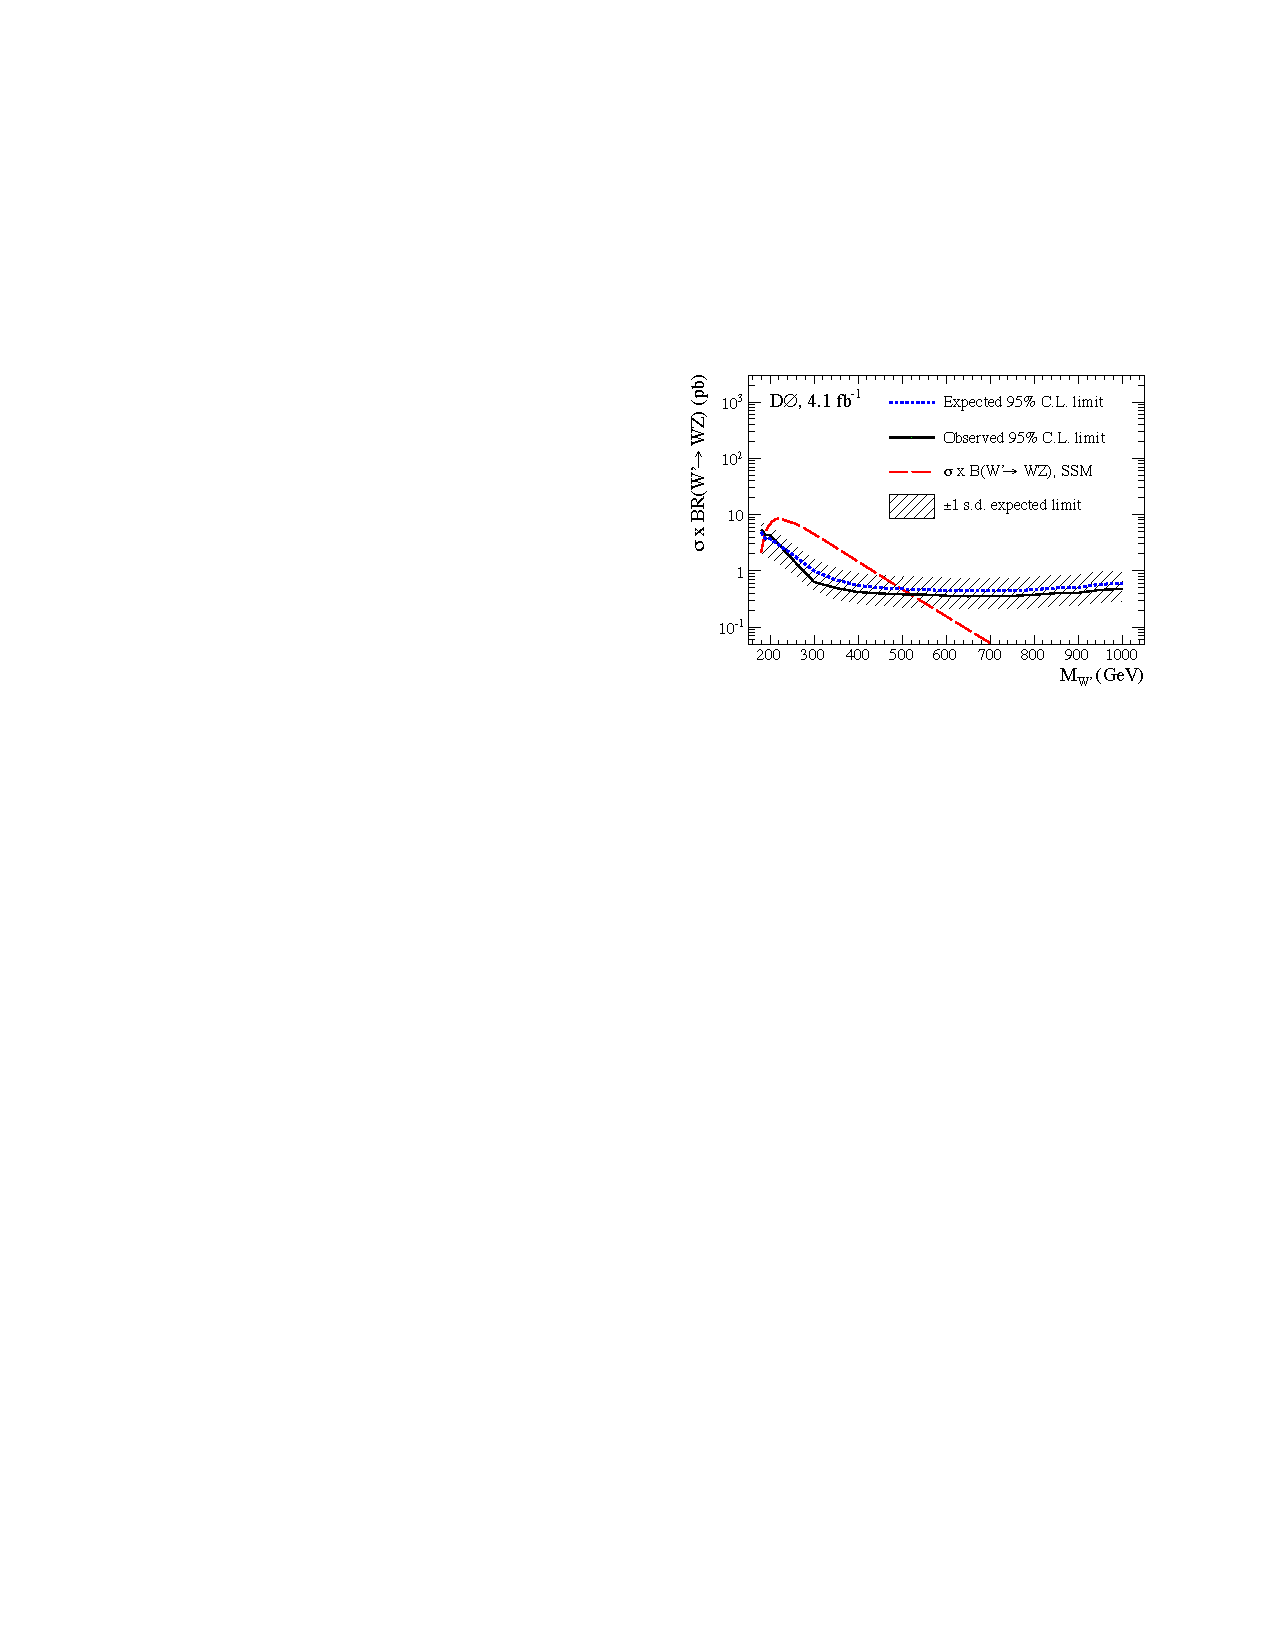
\includegraphics{figures/d0limit-wprime}
  \caption[\wprime limits from \dzero]{Limits on the cross section for \wprime production in the SSM based on results from \dzero{}.}
  \label{fig:d0limit-wprime}
\end{figure}

\begin{figure}
  \centering
  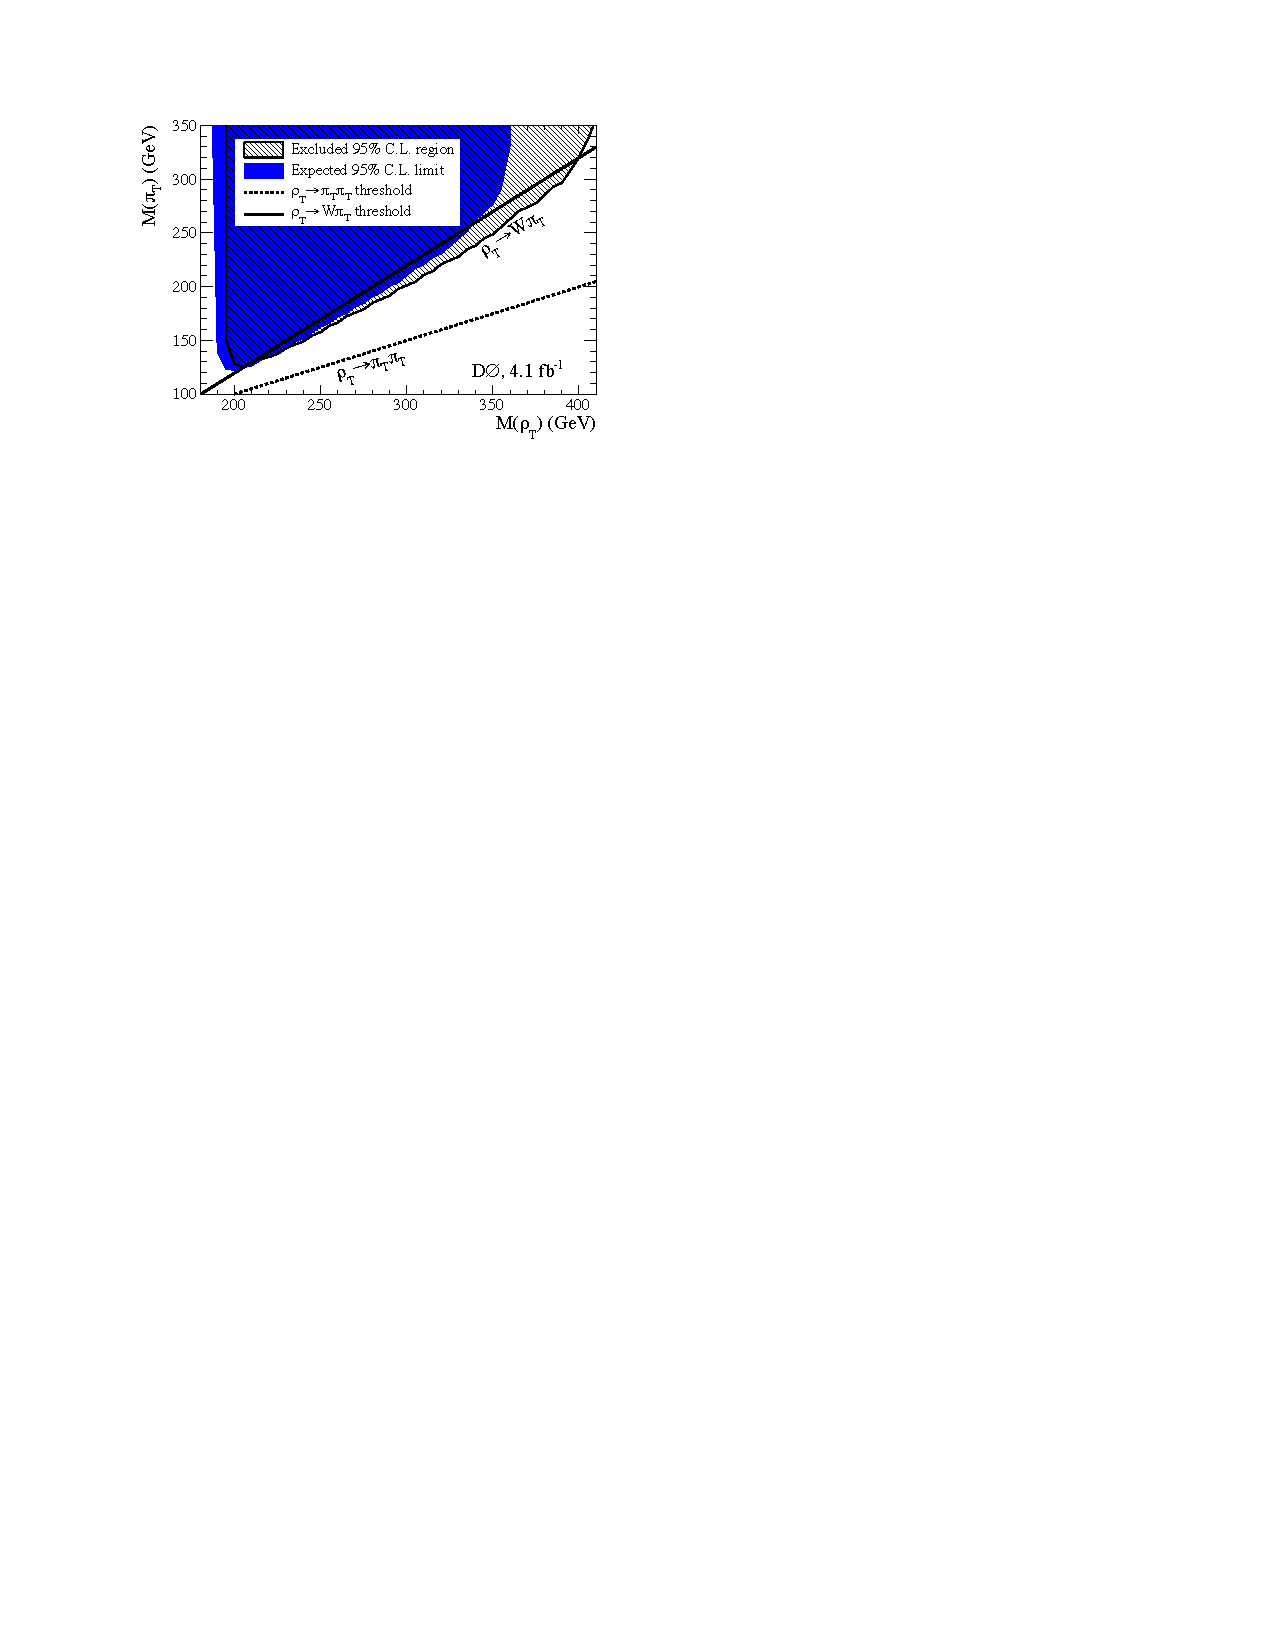
\includegraphics{figures/d0limit-tc}
  \caption[Technicolor limits from \dzero]{Excluded regions of technicolor parameter space based on results from \dzero{} with the thresholds of the $\technirho \to W + \technipi$ and $\technirho \to \technipi + \technipi$ decays overlaid.}
  \label{fig:d0limit-tc}
\end{figure}

For the resonance search, seeing that the number of observed events is consistent with SM predictions, the analysis proceeds to set limits on \wprime and technicolor models using a modified frequentist approach.  The limit-setting procedure relies on the transverse mass of the $WZ$ system to discriminate between signal and background, leading to results shown in Figures~\ref{fig:d0limit-wprime} and~\ref{fig:d0limit-tc}.  Within the SSM, they exclude a \wprime with mass in the range \simass{188} to \simass{520} at 95\% confidence level and find their results hold well in models with increased width of the \wprime{}.  Within technicolor models, they exclude a \technirho with mass in the range \simass{208} to \simass{408} under the assumption $M(\technirho) < M(\technipi) + M(W)$.

A comparison of this \dzero{} study to the potential for measurements at CMS closely follows the comparison made to CDF above.  The primary background at \dzero{} is from $ZZ$ rather than \Zjets and their cross section sensitivity is comparable to what has been achieved in the first results from CMS.  The higher energy of the LHC, however, makes a substantial difference in the reach for resonance searches with CMS, ruling out new sections of \wprime{} and Technicolor parameter space as discussed in Chapter~\ref{chapter:limits}.

% TODO: Talk about ATLAS results.

\resetlinenumber
% \chapter{Experimental Setup}
\label{chapter:experiment}

\section{The Large Hadron Collider}
In order to extend the energy frontier for collision experiments, the existing LEP tunnel was repurposed to house a new proton-proton machine, the Large Hadron Collider (LHC).  The \SI{26.7}{km} LEP ring consists of eight straight sections connected by eight arcs, housed at a depth of \SIrange{45}{170}{m} beneath farmland surrounding the Franco-Swiss border~\cite{Evans:1129806}.  The LHC is now the most powerful collider in the world, currently operating at a center-of-mass energy of \SI{8}{\TeV}, although this thesis considers only the 2011 runs at the slightly lower energy of \SI{7}{\TeV}.  The LHC operators plan to nearly double the collision energy by 2015.

Although a proton is nominally composed of only three quarks, its structure also involves gluons and $q\bar{q}$ pairs in continual flux.  Each of these constituents, including the short-lived components of the proton ``sea'', carries some fraction of the proton's overall momentum.  While the three valence quarks typically carry the largest portions, the antiquarks in the sea have some probability to fluctuate to comparable momenta.  Many previous hadron colliders have followed a $p\bar{p}$ design in order to maximize the possibility of high-energy valence $q\bar{q}$ interactions which have the possibility of generating a wide range of colorless final states.  The difficulty of producing antiprotons in large numbers, however, limits the achievable luminosity of such machines.  The $pp$ design of the LHC will allow it to attain luminosities many orders of magnitude beyond those seen at the Tevatron.  

The instantaneous luminosity for a symmetric colliding beam experiment such as the LHC is given as:
\begin{equation}
  \label{eq:luminosity}
  \mathcal{L} = \frac{n N^2 f}{A_\text{eff}}
\end{equation}
with $n$ the number of bunches per beam, $N$ the number of particles per bunch, $f$ the revolution frequency (\SI{11.246}{kHz}), and $A_\text{eff}$ the effective cross-sectional area of the beams.  The beams are focused to \SI{16}{\micro m} in each of the transverse directions ($\sigma_x$ and $\sigma_y$) which can be used to calculate the value of $A_\text{eff} = 4\pi \sigma_x \sigma_y$. The values of $n$ and $N$ have changed as the luminosity has progressed, so values are given by machine era in Table~\ref{tab:lhcparameters} while the total integrated luminosity delivered over the course of 2011 can be seen in Figure~\ref{fig:lumivstime}.

% The achieved luminosity is determined by various parameters of the beam as:
% \begin{equation}
%   \label{eq:luminosity}
%   \mathcal{L} = \frac{k N^2 f}{4\pi \sigma_x^{*} \sigma_y^{*}}
% \end{equation}
% where $k$ is the number of bunches per beam, $N$ is number of particles per bunch, $f$ is the revolution frequency (\SI{11.246}{kHz}), and $\sigma^{*}$ is the size of the beam at the collision point ($\sigma_x^{*} = \sigma_y^{*}$ = \SI{16}{\micro m}).  The values of these various parameters for given running periods are given in Table~\ref{tab:lhcparameters}.

\begin{table*}
  \centering
  \newcommand{\phan}{\phantom{0}}
  \begin{tabular}{l c c r c c}
    %http://lhc-commissioning.web.cern.ch/lhc-commissioning/
    \toprule
    Era & $E/\TeV$ & $\sqrt{s}/\TeV$ & $\mathcal{L}/(\si{cm^{-2}s^{-1}})$ & $N$ & $n$ \\
    \midrule
    Late \hfill 2010 & 3.5 & \phan 7 & \num{  2e32} & \num{e11} & \phan 348 \\
    Early       2011 & 3.5 & \phan 7 & \num{ 10e32} & \num{e11} & \phan 874 \\
    Late \hfill 2011 & 3.5 & \phan 7 & \num{ 30e32} & \num{e11} & 1318 \\
    Early       2012 & 4.0 & \phan 8 & \num{ 60e32} & \num{e11} & 1318 \\
    Design           & 7.0 &      14 & \num{100e32} & \num{e11} & 2835 \\
    \bottomrule
  \end{tabular}
  \caption[LHC operation parameters]{LHC operation parameters where $E$ is beam energy, $\sqrt{s}$ is center of mass energy, $\mathcal{L}$ is instantaneous luminosity, $N$ is the number of protons per bunch, and $n$ is the number of bunches per beam.  These numbers are only approximate, as the real luminosity progression has occurred in much smaller steps, with frequent tests of new configurations.}
  \label{tab:lhcparameters}
\end{table*}

\begin{figure*}
  \centering
  \includegraphics[width=\plotwidth]{matplotlib/lumivstime}
  \caption[Integrated luminosity recorded by the CMS detector vs.~time]{The integrated luminosity both \emph{delivered} by the LHC to CMS and \emph{recorded} by CMS in 2011.  The difference between delivered and recorded luminosities corresponds to a downtime less than 10\% for the CMS detector during the 2011 runs.}
  \label{fig:lumivstime}
\end{figure*}

The CERN accelerator complex includes a series of components which progressively accelerate the proton beams to higher energies.
The LHC makes use of the LEP injection chain to accelerate the protons to an energy of \SI{450}{\GeV} before entering the main ring.  
The first stage uses the Linac2 to boost the protons to \SI{50}{\MeV} in a series of radio frequency (RF) cavities, followed by similar pushes in the Proton Synchrotron Booster (PSB) to \SI{1.4}{\GeV} and then the Proton Synchrotron (PS) to \SI{24}{\GeV}.  In the PSB, magnets begin focusing the beam while its bunch structure is introduced in several steps through the PSB and PS stages.  The protons are brought up to a full injection energy of \sienergy{450} in the Super Proton Synchrotron (SPS).  Before taking on its current role as the main LHC injector, the SPS served as the colliding machine for its own round of new physics discoveries, delivering beam to the UA1 and UA2 experiments which first confirmed the existence of the $W$ and $Z$ bosons.  A schematic of these accelerator stages is available in Figure~\ref{fig:lhc-complex}.

\begin{figure*}
  \centering
  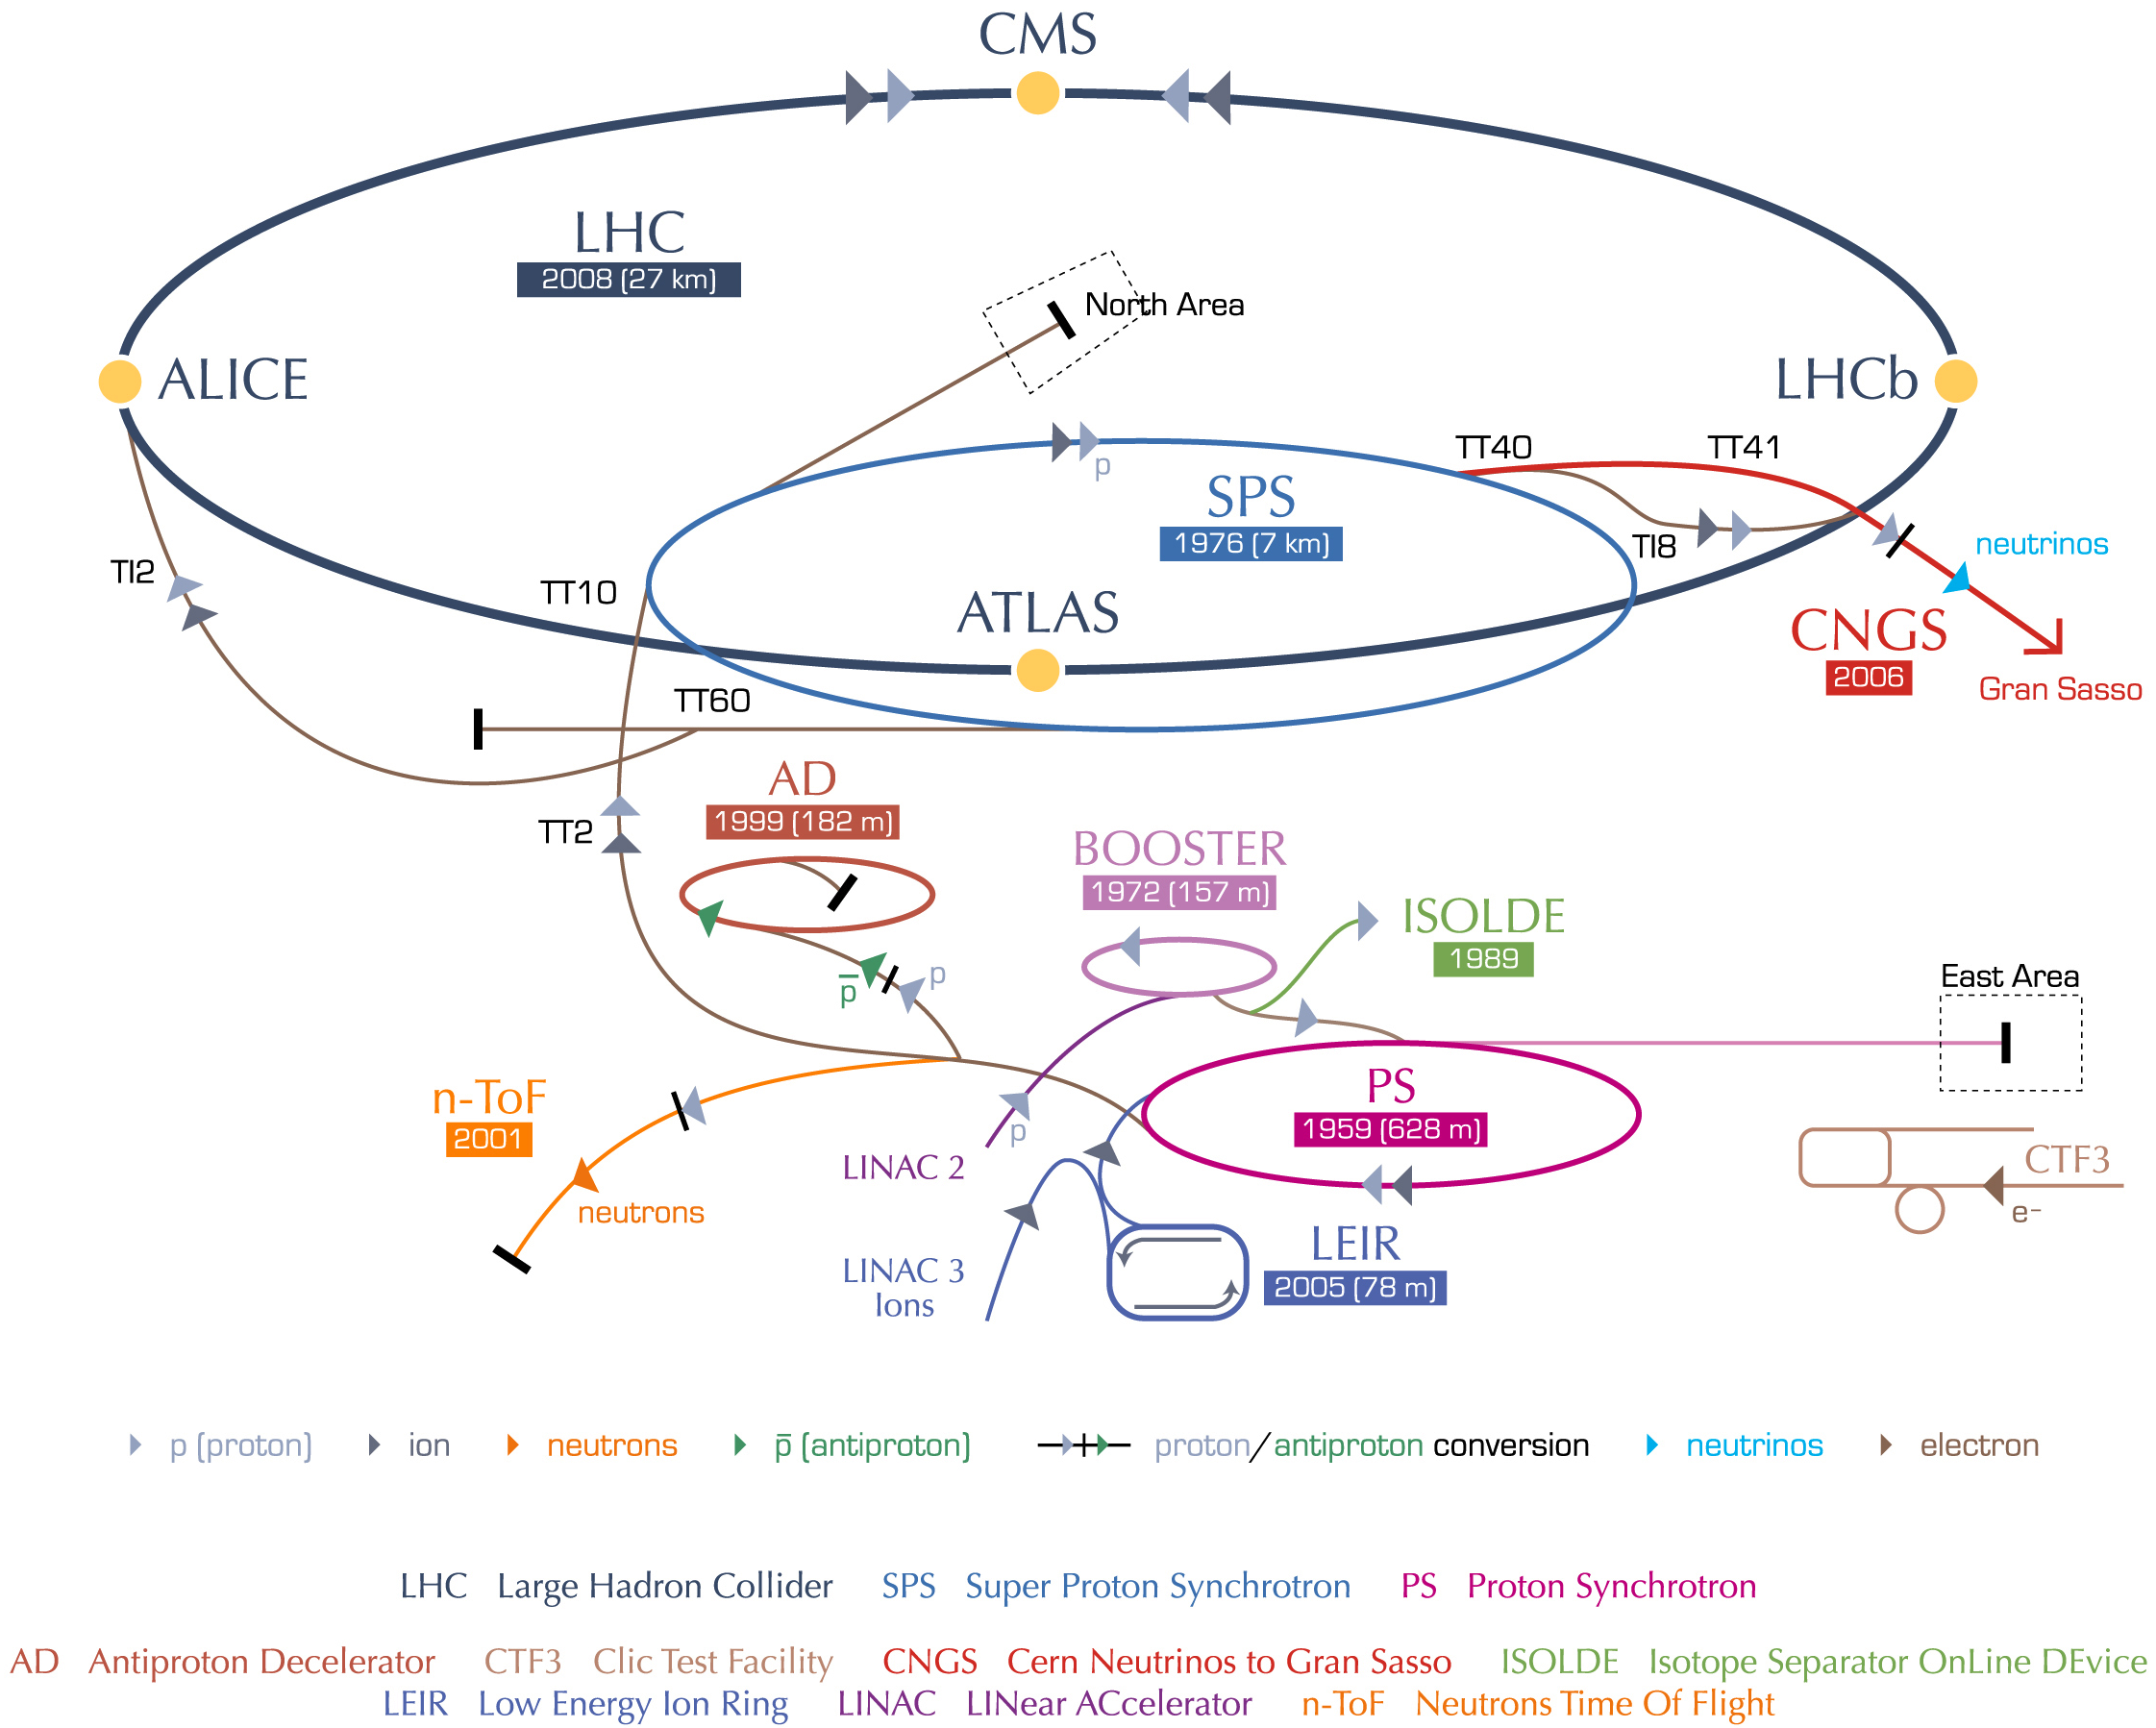
\includegraphics[width=\textwidth]{figures/cern-accelerator-complex-detail.png}
  \caption{Overview of the CERN accelerator complex.}
  \label{fig:lhc-complex}
\end{figure*}

The actual LHC ring consists of a pair of evacuated beampipes which pass through a series of bending and focusing magnets as well as RF cavities which boost and maintain the proton kinetic energy.  The magnets' unique twin-bore design produces oppositely-directed fields for the two counter-rotating beams of protons within a single structure, designed to provide the bending field of \SI{8}{T} necessary to confine a \SI{7}{TeV} proton beam in a ring of radius \SI{4.3}{km}.  While current technical difficulties have limited the achieved beam energy to \SI{4.0}{\TeV}, upgrades over the next several years are expected to bring the LHC magnets much closer to their design capacity.  A cryogenic system allows the magnets to avoid resistive losses by cooling them below \SI{2}{K} with liquid helium, bringing them into the superconducting regime.

\section{The Compact Muon Solenoid Experiment}
The analysis presented in this thesis relies on data collected with the Compact Muon Solenoid (CMS)~\cite{CMSPaper}, one of two general-purpose detectors installed in the LHC.  It has a broad physics reach as a result of a layered design with multiple calorimeter and tracking detectors arranged to complement one another and provide a nuanced view of collision events.  CMS earns its ``compact'' moniker by virtue of a novel design which fits both the electromagnetic and hadronic calorimeters inside of its solenoidal magnet, a goal which eluded the previous generation of detectors for hadron colliders. 
This design reduces energy loss and scattering for electrons and similarly energy loss for the converted photon allowing highly precise measurements of electrons and photons.
The arrangement of the subsystems can be seen in Figure~\ref{fig:cms-cutaway}.

The CMS design achieves hermetic coverage over a large solid angle by fitting endcaps on either side of a central barrel.  In most subsystems, there is sufficient overlap between the barrel and endcap such that particles can be well measured throughout the entire detector volume.

\begin{figure*}[htbp]
\centering
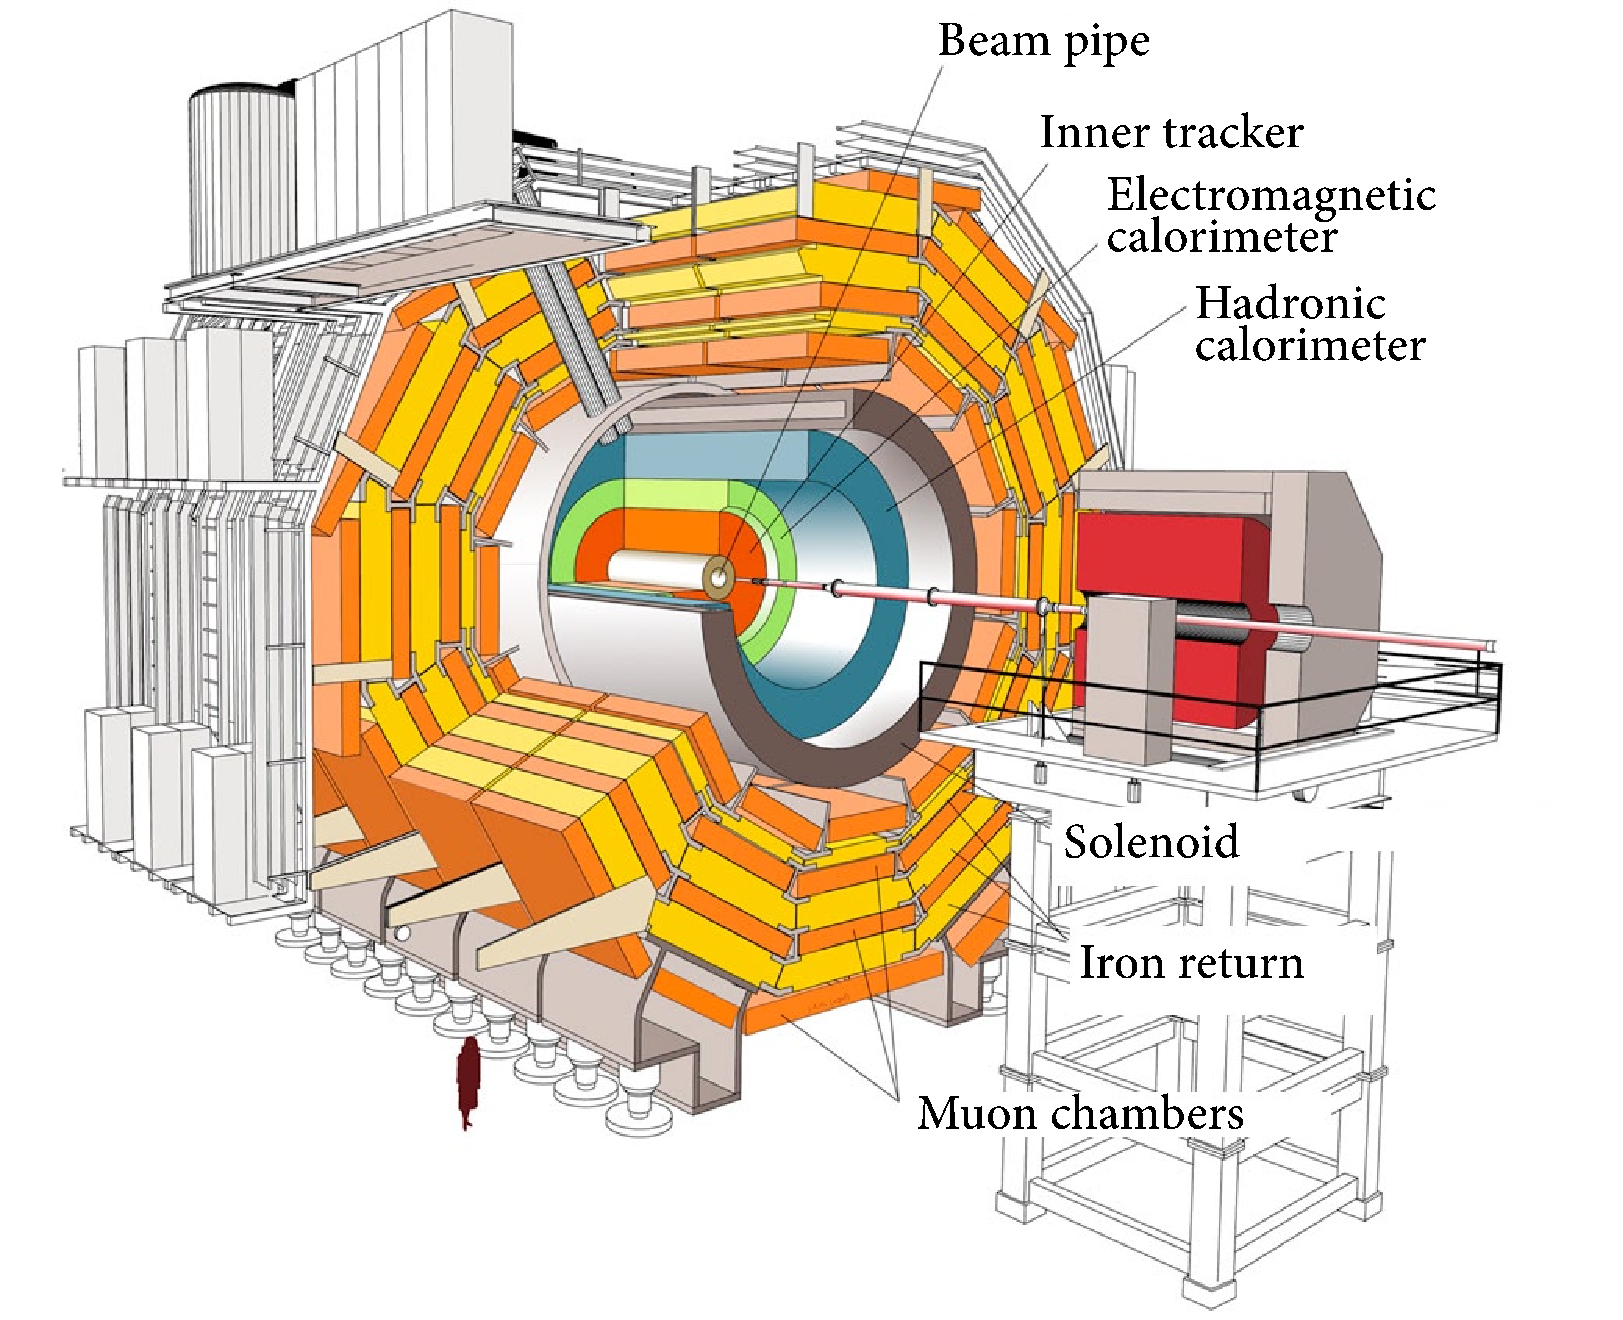
\includegraphics[width=4.5in]{figures/cms-cutaway.pdf}
\caption{A cut-away view of the barrel portion of the CMS detector with each of the main components labeled.}
\label{fig:cms-cutaway}
\end{figure*}

\subsection{Coordinate System}

% \begin{figure*}[!htbp]
%   \centering
%   \subbottom[Transverse view]{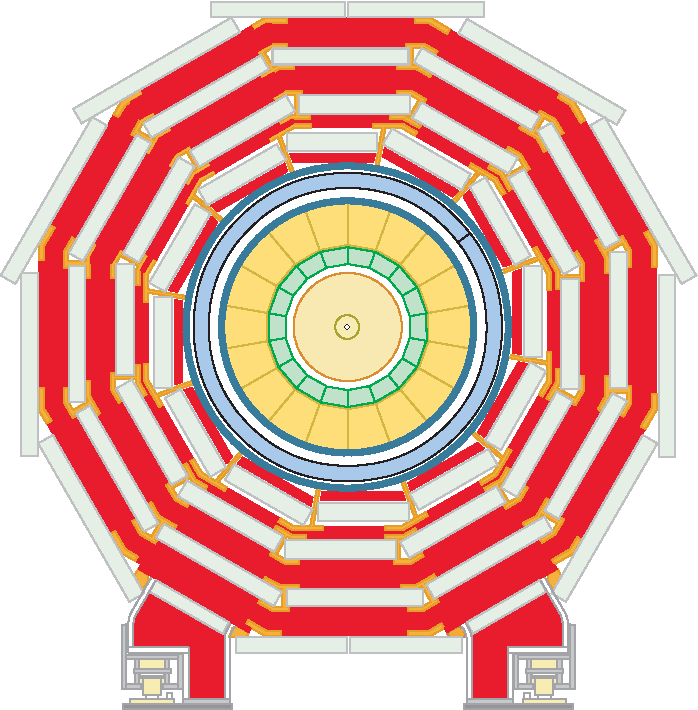
\includegraphics[width=0.35\textwidth]{figures/cms-xsection-trans.pdf}\label{cms-xsection-trans}}
%   \subbottom[Longitudinal view]{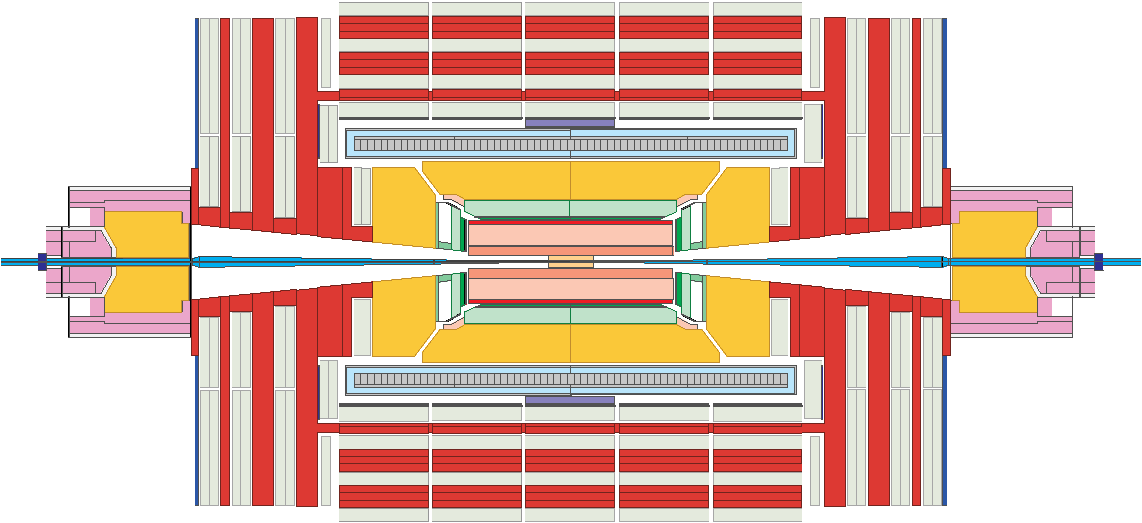
\includegraphics[width=0.65\textwidth]{figures/cms-xsection-long.pdf}\label{cms-xsection-long}}
%   \caption{Two cross-sectional views of the \cms detector.}
%   \label{cms-xsections}
% \end{figure*}

\begin{figure*}
  \centering
  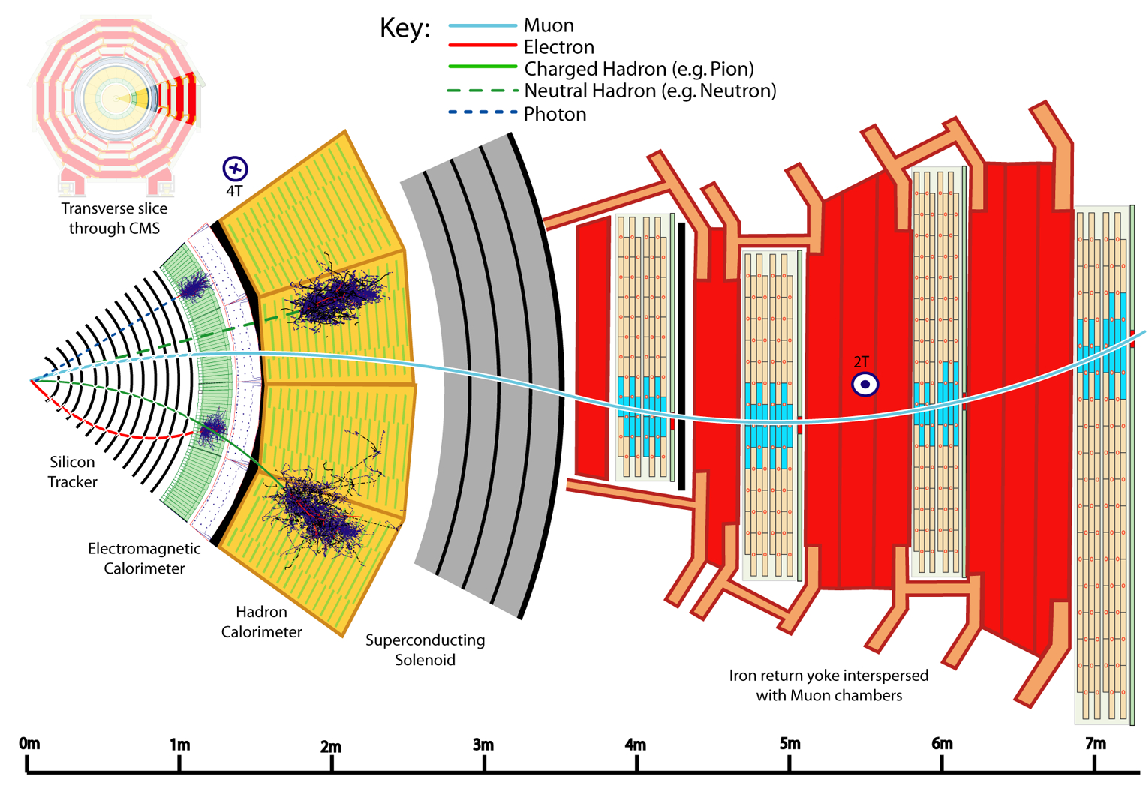
\includegraphics[width=\textwidth]{figures/cms-slice}
  \caption{A transverse slice of the CMS detector, showing the various subsystems and expected behavior of muons, electrons, photons, and hadrons.}
  \label{cms-xsections}
\end{figure*}

A location within the \cms detector can be described using a typical right-handed cartesian coordinate system originating from the center of the detector.  The $x-y$ plane forms a vertical cross section with the $y$-axis pointing upward and the $x$-axis pointing south toward the center of the LHC ring.  The $z$-axis points west, following the direction of the counter-clockwise proton beam as viewed from above.  Particles produced in collision events originate near the center of the detector and move quickly outward in all directions; for our measurements, then, we typically are concerned with the angle of the particle's initial trajectory away from the center of the detector.  To this end, we define the azimuthal angle $\phi = \arctan(y/x)$ and the polar angle $\theta = \arctan(\sqrt{x^2 + y^2}/z)$.

The products of 2-to-2 collisions mediated by the strong force, accounting for the vast majority of events produced by the LHC, tend to have momenta much larger along the $z$-axis than transverse to it, rendering the polar angle an inconvenient description for deviation from the beam pipe.  Particle physicists have traditionally defined a \emph{rapidity} relative to the beam axis,
\begin{equation}
  y \equiv \frac{1}{2}\ln\left(\frac{E + p_z}{E - p_z}\right),
\end{equation}
which in the relativistic limit ($E \approx |\vec{p}|$) reduces to a simple function of the polar angle,
\begin{equation}
  \label{eq:pseudorapidity}
  \eta = - \ln\left(\tan{\theta \over 2}\right).
\end{equation}
This quantity (known as \emph{pseudorapidity}) proves most convenient for describing deflection from the beam axis because the occupancy of the detector is approximately constant in equal $\eta$ intervals.  One of the distinguishing features of interactions that produce massive particles is that the decay products tend to be produced in a more spherical distribution, motivating a detector design with the best instrumentation in the central region of pseudorapidity.

\subsection{Solenoidal Magnet}
Much of the CMS design is driven by the desire to provide precise momentum measurements in the \TeV regime.  For a particle of charge $q$, the transverse momentum can be inferred from the radius of curvature of its trajectory ($r$) when it moves through a magnetic field $B$:
\begin{equation}
  \label{eq:curvature}
  \pt = q r B.
\end{equation}
The resolution of the radius measurement depends on the amount of curvature, so as particles move towards higher energies, the momentum resolution degrades.  In order to provide sufficient bending even for \TeV-scale particles, CMS was designed with the most powerful magnet built to date, sustaining a homogenous \SI{3.8}{T} magnetic field over a volume of more than \SI{300}{m^3}.  The return field saturates the iron yoke, providing a consistent \SI{2}{T} field throughout the outer muon system, allowing an additional, large lever arm measurement of the transverse momentum for highly penetrating particles such as muons.  The capabilities and geometry of the magnet guide the design of each of the CMS subsystems.

\subsection{Inner Tracker}

Starting from the beampipe and moving outward into CMS, the first instrumented region is the inner tracking detector.  The entire inner tracker is based on a silicon semiconductor design.  As charged particles traverse the tracker, they deposit ionization energy, dislodging electrons which in turn produce secondary ionization.  The semiconducting silicon is held at a high voltage, causing the released electrons and corresponding holes to separate.  The electrons are collected as an electric pulse, with some threshold applied to indicate a ``hit'', or the passage of a charged particle through a particular region of silicon. 

The primary role of the inner tracker is to provide precise measurements of the trajectories of all charged particles.  Its resolution, however, is also sufficient to distinguish a secondary vertex in a single collision event corresponding to displaced tracks which are the hallmark of the relatively short-lived hadrons containing $b$ or $c$ quarks; this allows discrimination between prompt leptons produced from the decay of vector bosons and secondary leptons produced in the semileptonic decays of hadrons.  The total tracker system, \SI{5.8}{m} in length and \SI{2.5}{m} in diameter, consists of silicon pixels and strips, arranged in various layers, and covers the pseudorapidity region $-2.5<\eta<2.5$.

The first three layers (out to a radius of \SI{10.2}{cm}) consist of silicon pixels which provide maximum precision and granularity for the extremely high particle occupancies expected in a region so close to the interaction point~\cite{Kastli2007724}.  Each of the approximately 66 million pixels is $\SI{100}{\micro m} \times \SI{150}{\micro m}$ in size, leading to a total coverage of \SI{1}{m^2}.  The pixels provide tracking points in both the $r-\phi$ (resolution $~\SI{10}{\micro m}$) and $r-z$ (resolution $~\SI{20}{\micro m}$) planes.  The design's emphasis on providing a $z$ resolution on par with the $r-\phi$ resolution is the key feature which allows successful secondary vertex reconstruction in three dimensions.

\begin{figure*}
  \centering
  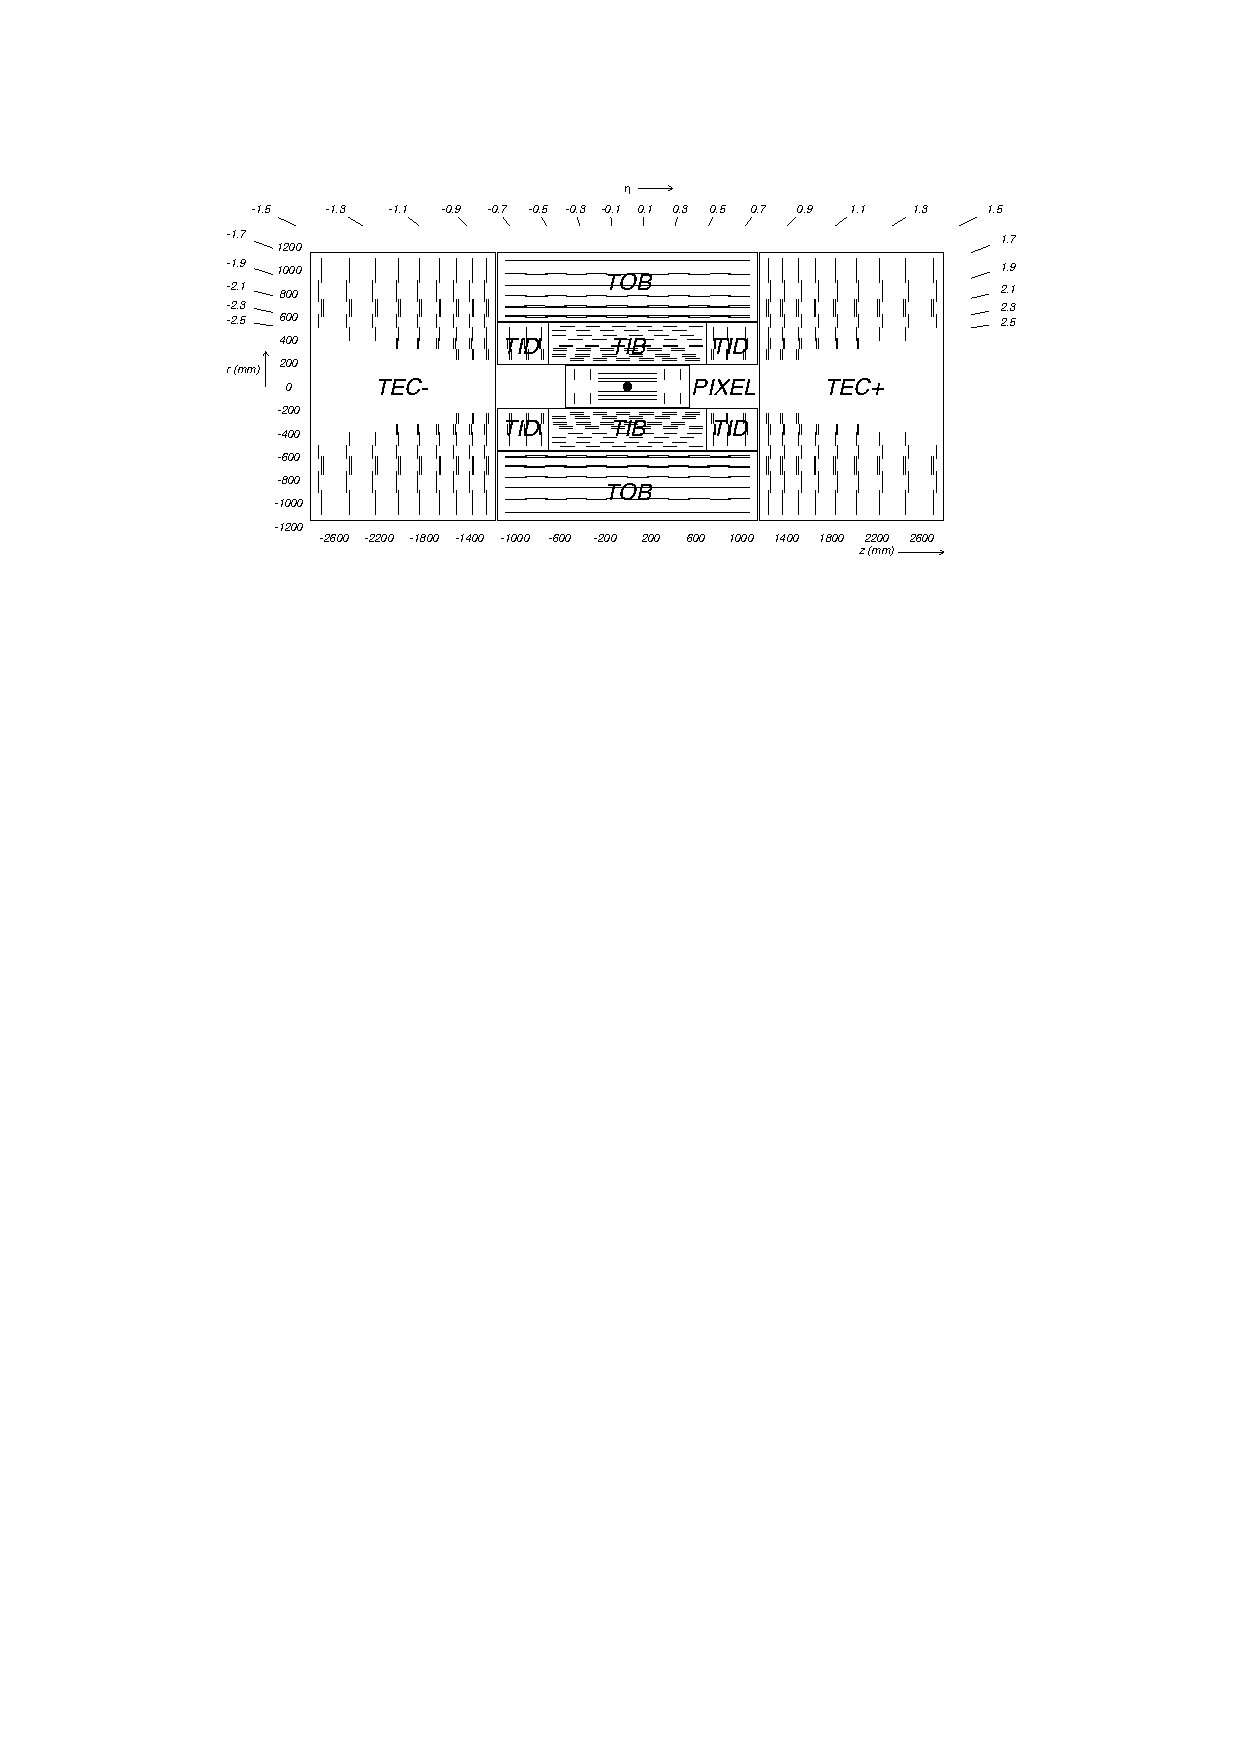
\includegraphics[width=\textwidth]{figures/cms-tracker-xsec.pdf}
  \caption[Schematic cross section through the CMS tracker]{Schematic cross section through the CMS tracker.  Each line represents a detector module.  Double lines indicate back-to-back modules which deliver stereo hits~\cite{Evans:1129806}.}
  \label{fig:tracker-xsec}
\end{figure*}

Outside the pixel system lie ten layers of silicon microstrip detectors, each strip \SI{10}{cm} to \SI{25}{cm} long with a height of \SI{180}{\micro m} and spacing between the strips (known as ``strip pitch'') varying by region.  The strips are distributed across two barrel regions, the tracker inner barrel (TIB, strip pitch of \SI{80}{\micro m} to \SI{120}{\micro m}) and the tracker outer barrel (TOB, strip pitch of \SI{120}{\micro m} to \SI{190}{\micro m}), along with two endcap regions, the tracker inner disks (TID) and the tracker endcaps (TEC) with radial strips of \SI{97}{\micro m} to \SI{184}{\micro m} average pitch.  The overall layout of the tracker subsystems can be seen in Figure~\ref{fig:tracker-xsec}.

Hits in the silicon pixels and strips are used as input to reconstruction algorithms which connect them together into tracks and calculate the associated momenta.  The momentum resolution of the tracker is 
\begin{equation}
  %\frac{\sigma(\pt)}{\pt} = \frac{\pt}{\GeV} \cdot 0.015\% \oplus 0.5\%
  \frac{\sigma(\pt)}{\pt} = (\pt/\GeVc) \cdot 0.015\% \oplus 0.5\%
\end{equation}
for $|\eta| < 1.6$, with the relative error increasing in the forward region to a maximum of
\begin{equation}
  %\frac{\sigma(\pt)}{\pt} = \frac{\pt}{\GeV} \cdot 0.060\% \oplus 0.5\%
  \frac{\sigma(\pt)}{\pt} = (\pt/\GeVc) \cdot 0.060\% \oplus 0.5\%
\end{equation}
for $|\eta| = 2.5$.  The first term accounts for the curvature measurement which becomes less precise for high-momentum tracks that bend only slightly in the magnetic field.  The second term accounts for interactions with the tracker material such as multiple scattering.

\subsection{Electromagnetic Calorimeter}
\label{sec:ecal}

\begin{figure*}
  \centering
  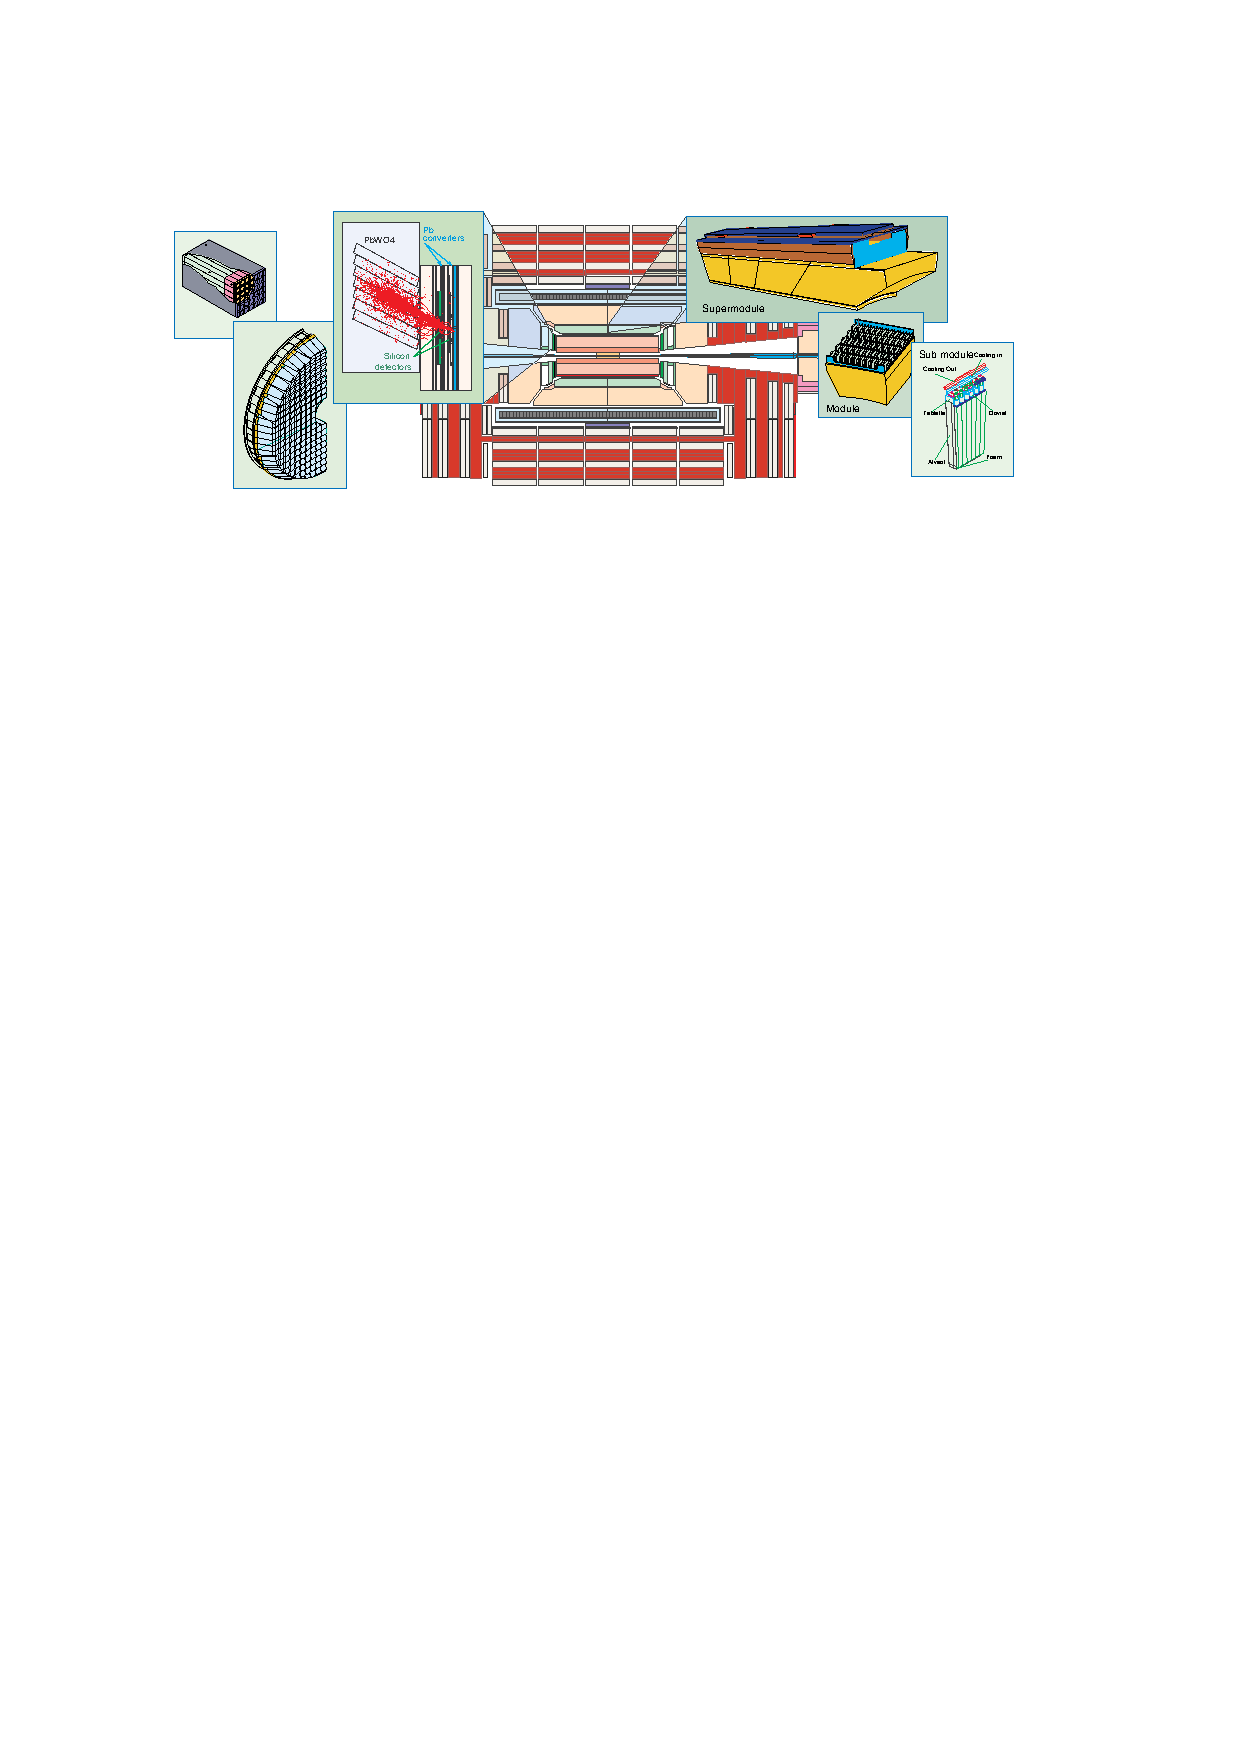
\includegraphics[width=\textwidth]{figures/cms-ecal}
  \caption{A schematic showing the various features of the CMS \ecal.}
  \label{fig:cms-ecal}
\end{figure*}

The CMS electromagnetic calorimeter (\ecal) is designed to detect electrons and photons, inducing electromagnetic showers and collecting the resultant photons.  The \ecal{} is able to achieve a remarkably high energy resolution due both to the homogenous coverage provided by a crystal-based design and to its location inside the solenoid, avoiding the significant degradation seen in previous hadron collider experiments due to interactions in the magnet material.  To keep the solenoid a reasonable size, however, the \ecal{} must be incredibly compact, necessitating a dense interaction material which maintains transparency under high doses of radiation so that photons can reach a collection region with minimal energy loss.  Lead tungstate (\leadtungstate) crystals provide a high density (\SI{8.28}{g/cm^3}), short radiation length (\SI{0.89}{cm}), and small Moli\`{e}re radius (\SI{2.2}{cm}), leading to rapidly progressing, tightly contained showers for high-energy electrons and photons.  The crystals emit a blue-green scintillation light peaking near \SI{425}{nm}, which is collected by avalanche photodiodes (APDs) and vacuum phototriodes (VPTs).  The APDs and VPTs produce electrical signals which correlate with the multiplicity of detected photons, allowing us to calculate ``energy deposits'' left in each crystal.  A schematic is provided in Fig.~\ref{fig:cms-ecal}.

The \ecal barrel (EB) offers pseudorapidity coverage to $|\eta| < 1.479$ through use of \num{61200} crystals, each with a tapered shape of roughly $\SI{22}{mm} \times \SI{22}{mm}$ at the front face, widening to $\SI{26}{mm} \times \SI{26}{mm}$ at the rear, and with a \SI{230}{mm} length of which provides approximately 26 radiation lengths of material. The precise shape of the crystals is slightly different in various $\eta$ regions.  The EB crystals are arranged into modules ($~500$ crystals) and supermodules (1700 crystals) which various structural and readout elements.

The \ecal endcaps (EE) cover a pseudorapidity range $1.479 < |\eta| < 3.0$ through use of \num{14648} identically-shaped crystals, again with a tapered design widening from $\SI{28.62}{mm} \times \SI{28.62}{mm}$ at the front face to $\SI{30}{mm} \times \SI{30}{mm}$ at the rear, with a \SI{220}{mm} length corresponding to 25 radiation lengths.  They are grouped into $5 \times 5$ mechanical units called supercrystals.

Energy deposits in individual crystals are combined into clusters of energy, which are further grouped into superclusters in the reconstruction algorithms, serving as the starting point for identification of electrons and photons in the detector.  The \ecal achieves an energy resolution given as:
\begin{equation}
  \frac{\sigma(E)}{E} = \frac{1}{\sqrt{E/\GeV}} \cdot 2.8\% \oplus \frac{1}{E/\GeV} \cdot 0.0415\% \oplus 0.3\%
\end{equation}
where the three terms correspond to statistical fluctuations and intrinsic shower fluctuations; electronic noise and pileup energy; and detector non-uniformity and calibration uncertainties.

\subsection{Hadronic Calorimeter}

\begin{figure*}
  \centering
  \includegraphics[width=\textwidth]{figures/cms-hcal}
  \caption{A schematic showing the various features of the CMS \hcal.}
  \label{fig:cms-hcal}
\end{figure*}

The CMS hadronic calorimeter (\hcal) is designed to detect particles which primarily interact with atomic nuclei via the strong force.  Measurement of the energy of such particles is particularly import for the reconstruction of jets of hadrons and missing transverse energy, which could indicate the presence of neutrinos or long-lived neutral exotic particles in collision events.  Strongly interacting particles typically start showering in the dense material of the \ecal{}, so a full picture of a jet's energy relies combining information from both the electromagnetic and hadronic calorimeters.  

The basic design of the \hcal is a sampling calorimeter with alternating layers of brass and scintillator.  The brass acts as a non-ferromagnetic absorber, capable of withstanding the intense magnetic field, providing \num{5.82} interaction lengths of material in the barrel to encourage development of hadronic showers.  The scintillator consists of tiles along with wavelength-shifting fibre.  Hadrons interact with the scintillating material to produce a broad spectrum of photons which are then absorbed in the fibre and re-emitted in a more narrow range to which the photodetectors are sensitive.  In the endcap, brass is replaced with steel and tile with quartz, which are both better able to withstand the higher radiation dose in that region.  A schematic is provided in Fig.~\ref{fig:cms-hcal}.

The resolution for the barrel and endcap \hcal ($|\eta| < 3.0$) is given as:
\begin{equation}
  \frac{\sigma(E)}{E} = \frac{1}{\sqrt{E/\GeV}} \cdot 85\% \oplus 7.4\%
\end{equation}
with stochastic and constant terms in analogy to those discussed for the \ecal.  The inferior performance relative to the \ecal is due both to its operating principle of sampling the shower rather than absorbing all produced energy in high-resolution crystals and also to the intrinsically lower particle multiplicity in hadronic showers vs.\ electromagnetic showers, leading to wider statistical fluctuations.

\subsection{Muon System}

\begin{figure*}
  \centering
  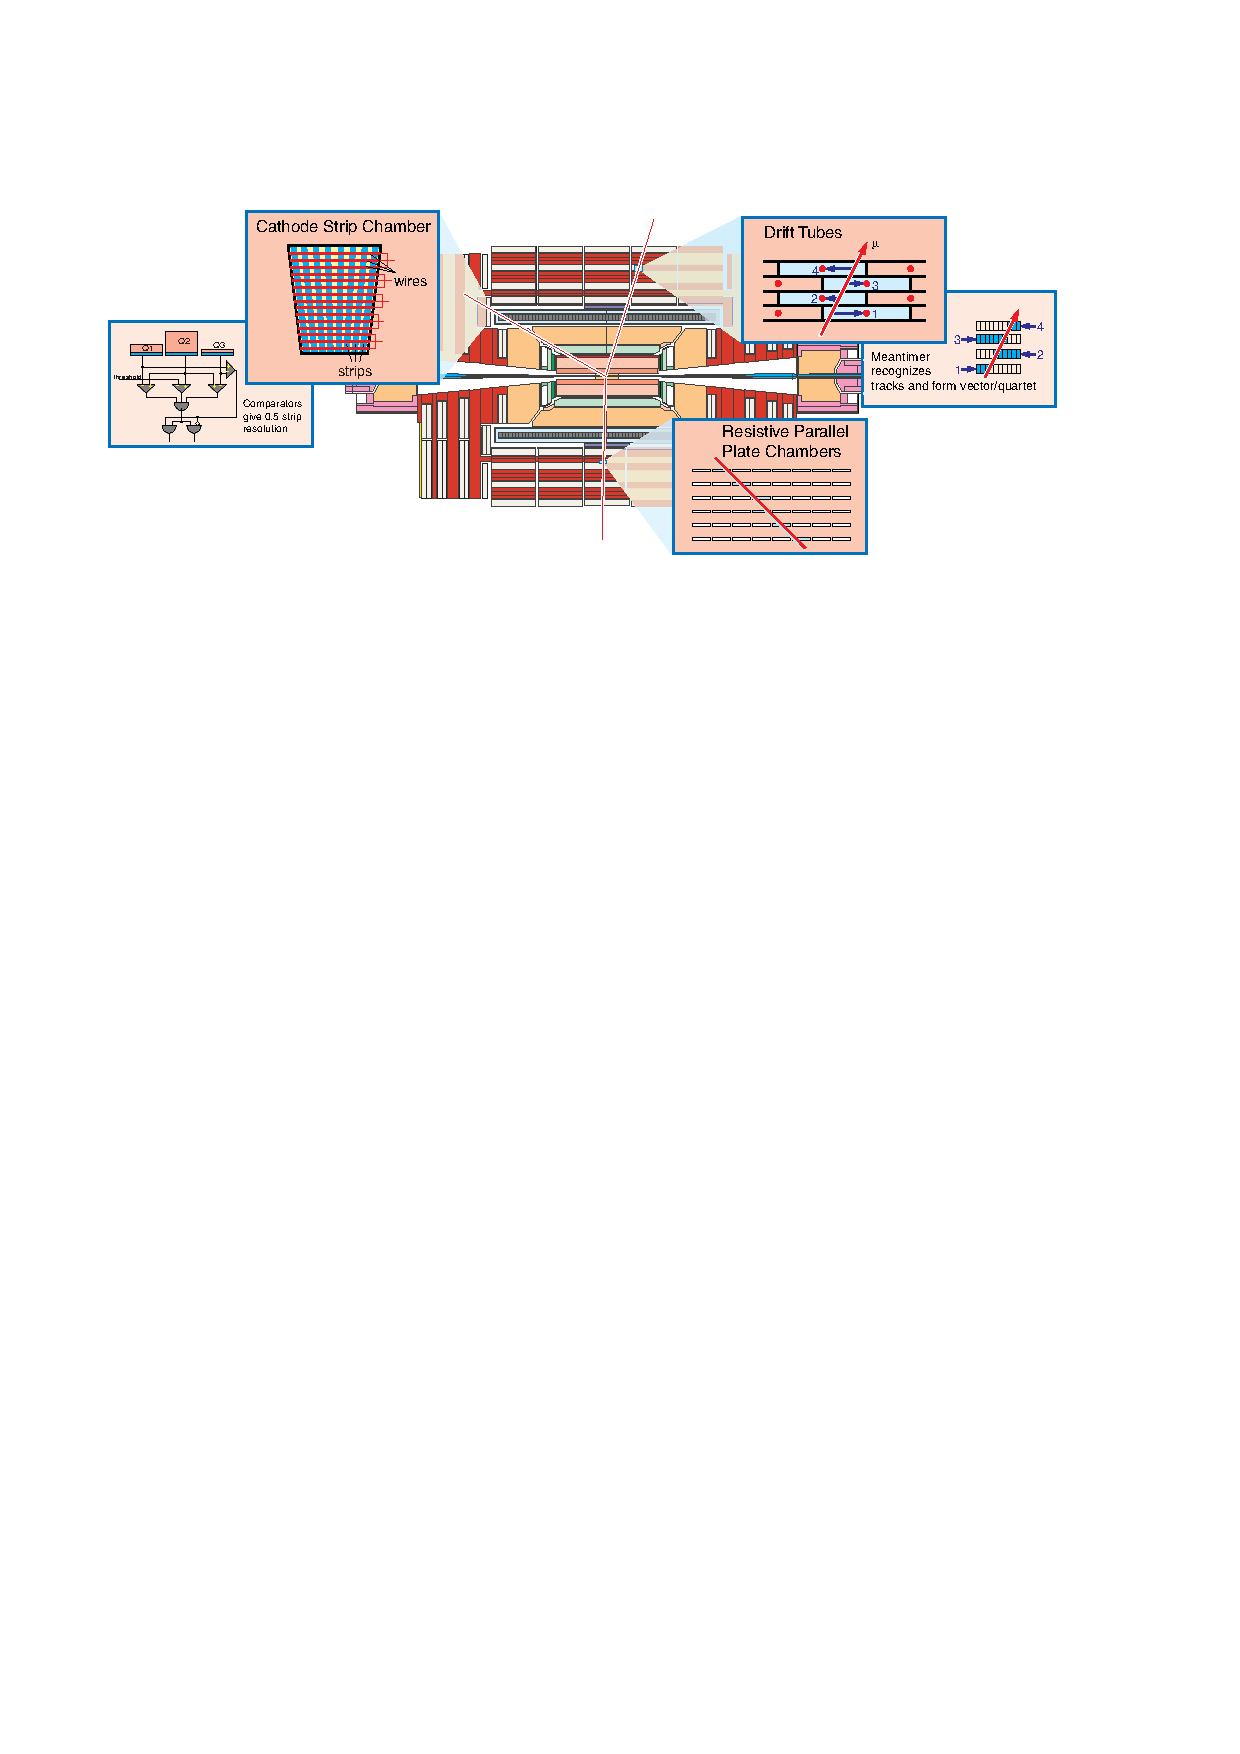
\includegraphics[width=\textwidth]{figures/cms-muon-system}
  \caption{A schematic overview of the various muon detector technologies.}
  \label{fig:cms-muon-system}
\end{figure*}

As suggested by its name, the Compact Muon Solenoid is designed with the detection of muons as a high priority.  As such, it includes an advanced muon spectrometer capable of distinguishing muons with high accuracy and contributing to an impressive momentum resolution for energetic muons.  The muon system employs three types of gaseous particle detectors optimized for different environments and goals -- drift tubes (DTs) in the barrel, cathode strip chambers (CSCs) in the endcaps, and resistive plate chambers (RPCs) covering nearly the entire barrel and endcap regions.

Muon chambers are arranged in 4 stations embedded in a heavy iron yoke with each consecutive station located further from the interaction region.  The iron yoke provides a support structure for the various chambers and concentrates the return field of the solenoid in order to provide significant bending of muons for the momentum measurement.  A schematic showing the layout of the muon system is provided in Fig.~\ref{fig:cms-muon-system}.

DTs consist of chambers filled with a gas mixture ionized by the passage of charged particles.  Within each chamber is a wire held at high voltage, setting up an attracting electric field to collect the ionization charge, producing an electric pulse in the wire indicating the presence of a particle.  Because the drift velocity for electrons in a particular gas mixture is well defined, a drift tube can provide a precise measurement of the particle's position based on the drift time of the collected charge. These chambers are an economical and robust choice as the primary muon system detector in the CMS barrel, a region with low occupancy and modest magnetic field, but they have a relatively slow response (drift time up to \SI{380}{ns}) which disqualifies them for use in the more active endcap region.  The sensitive wires in each tube are \SI{2.4}{m} long and the gas is a mixture of argon and carbon dioxide.  Each DT chamber consists of three superlayers, each composed in turn of four layers of rectangular drift cells staggered by half a cell.  The two outer superlayers are oriented with the wires parallel to the beam to provide tracking in the $r-\phi$ plane in which the muon bends due to the magnetic field.  The third superlayer, present only in the first three stations, measures the $z$ coordinate.

The higher occupancy of the endcap regions requires the fast performance and high granularity of CSCs.  The CSC is a type of multiwire proportional chamber where a plane of multiple anode wires is housed within a single gas chamber, with each wire acting as an individual proportional counter.  The wires are held at voltage, providing an electric field such that the electrons produced by ionization due to a passing charged particle are drawn to the wires, producing an electric signal indicating the particle's presence.  The CMS endcaps contain a total of 468 CSCs, each comprised of six anode wire planes interleaved among 7 cathode panels.  All wires run azimuthally, with the $\phi$ coordinate localized by interpolating charges induced on the strips.  

An RPC~\cite{Santonico1981377} consists of parallel electrode plates, setting up a constant and uniform electric field across an ionizing gas in the gap.  The electrodes are constructed with a high resistivity such that the electric field is suddenly switched off when a charged particle causes an ionization discharge in the gas, preventing the charge from propagating through the gas.  The uniform field design yields a much better time resolution than wire chambers with a $1/r$ field dependence around each wire.  The RPCs installed in the CMS muon system employ a double-gap design operating in avalanche mode and although they cannot compete with either the DTs or the CSCs for spatial resolution, their superior timing resolution is fine enough to unambiguously associate muon hits to a particular bunch crossing, even with the high rate and pileup of the full LHC luminosity.  As such, they are useful in triggering muon events.

\subsection{Trigger System}

At design luminosity of the LHC, we expect beam crossings at a frequency of \SI{40}{MHz} leading to collisions on the order of one billion per second delivered to CMS, allowing unprecedented access to rare physics events.  Ideally, we would like to be able to keep a record of every delivered collision, but no data acquisition or storage system available with current technology would be able to deal with even a hundredth of the requisite rate.  Most events at the LHC, however, consist only of ``soft'' collisions without a significant momentum transfer, producing final states with low-energy jets which have been extensively studied at lower-energy colliders and are unlikely to reveal new physics insights.  By ignoring these low-energy events, we can define a more tractable stream of collisions with higher likelihood for interesting content.  Determining which events to keep, however, requires a specialized ``trigger'' system capable of making sub-millisecond decisions about the physics potential of incoming events.

The CMS trigger system uses custom hardware combined with a computing farm to achieve a million-fold reduction in the stored event rate.  The hardware step, called the level-1 (L1) trigger, is designed with an output rate of \SI{100}{kHz}, using coarsely binned information from the detector to quickly detect any potentially interesting physics content in an event.  Events selected by L1 are passed to the high-level trigger (HLT), where commercial computing nodes run speed-optimized reconstruction algorithms in order to further reduce the event rate to a target of \SI{300}{Hz} to \SI{400}{Hz} for permanent storage.

\subsection{Luminosity Measurement}

The LHC machine cannot itself measure the luminosity of proton collisions, so the CMS detector itself must be used to perform a measurement, leading to one of the largest sources of error in cross section measurements and in new particle searches.  As a result, much attention has been paid to providing a reliable and precise luminosity measurement at CMS.  

Through 2011, CMS had been using a luminosity determination~\cite{LUMIPAS} based on activity in the forward hadronic calorimeter (HF) which covers the pseudorapidity range $3 < |\eta| < 5$ to record the transverse energy of forward jets.  The primary technique involves ``zero counting'' where the mean number of interactions per bunch crossing is inferred from the average fraction of empty calorimeter towers.  The technique requires calibration through a Van der Meer scan where the size and shape of the interaction region is measured by recording the relative interaction rate as a function of the transverse beam separations~\cite{vanderMeer:296752}.  This Van der Meer calculation includes a dependence on the LHC beam currents, which are only known to an accuracy of 3.1\%~\cite{Alice:1333997}, which becomes the primary contributor to the total uncertainty of 4.5\% on the luminosity measurement.

The new luminosity measurement approved in early 2012~\cite{CMS-PAS-SMP-12-008} relies on a calibration procedure based on cluster counting in the pixel tracker.  Because of the very fine granularity of the pixel tracker, the probability of a given pixel being hit by two different tracks in one bunch crossing is small, meaning that the number of clusters per crossing should vary linearly with the number of interactions per crossing and thus the luminosity.  This technique also requires a Van der Meer scan, but here the calibration involves monitoring pixel activity with less acute dependence on the LHC beam current, allowing a precise determination of the effective pixel cluster cross section.  That cross section is then applied to determine an instantaneous luminosity for each luminosity section (corresponding to \SI{23.3}{s} of collisions) of the 2011 physics data sample based on the level of activity in the pixels.  The new method achieves a total systematic uncertainty of 2.2\%.

\resetlinenumber
% \chapter{Event Simulation}
\label{chapter:simulation}

\section{The Monte Carlo Approach}

In order to understand rare collision events, experimentalists must be able to sort through trillions of collisions to find perhaps only a handful of interesting candidates.  Resolving these events would be impossible without firm theoretical predictions to guide us in deciding what exactly to look for.  It is no simple task, however, to map the equations defining the differential cross sections for various processes onto the discrete event structure of experimental data.  To bridge this gap, we generally use ``Monte Carlo'' techniques~\cite{MonteCarloMethod} where a random number generator is interfaced with the equations governing a certain process in order to produce a large number of simulated collision events.

In practice, simulated data may pass through several different programs, with each specialized to emulate a particular aspect of particle collisions.  The first stage is a matrix element calculation which describes the differential cross section for a given \emph{hard scattering} process or for a set of interfering processes with the same initial and final states (such as in Drell-Yan production of leptons, $q\bar{q} \to \ell^+ \ell^-$, which can be mediated by either a photon or a $Z$ boson~\cite{PhysRevLett.25.316}).  If some of the final-state particles from this initial process are short-lived (such as the vector bosons), their decays will be directly handled in the same calculation due to additional interference possibilities.  For particles with finite lifetimes on the scale of a muon or a tau lepton, decays can be decoupled from the calculation and are generally handled at a subsequent stage.  These later-stage programs choose decays according to branching ratios which are derived primarily through measurements from previous experiments.

Another program takes the colored \emph{partons}---quarks and gluons---produced in the hard scattering interaction along with any radiated gluons and describes how they hadronize into colorless composite particles in a \emph{parton showering} process.  Still another program describes the \emph{underlying event} consisting of soft interactions of the \emph{spectator} partons which did not directly participate in the hard scattering. These programs rely on parameterizations tuned first by input from previous colliders extrapolated to LHC energies and later retuned based on data from initial LHC runs~\cite{Moraes:2007rq,springerlink:10.1007/JHEP01(2011)079}.

\section{Parton Distribution Functions}
Hadron colliders cannot be tuned to take advantage of resonant production because collisions take place at the parton level.  Although each proton carries a well-constrained momentum, the distribution of that momentum amongst its constituents is constantly in flux.  As a result, each hard scattering interaction is unique and a computer simulation must seek to faithfully model both individual scattering interactions with the relevant probabilities along with the aggregate behavior of an ensemble of interactions.  Programs simulating hard scattering events are guided by \emph{parton distribution functions} (PDFs) which describe the relative probability for each parton type to be carrying a particular momentum fraction $x$.  Current calculative ability in QCD is insufficient to predict these distributions, so they are measured experimentally by fits to deep inelastic scattering, production of electroweak bosons, and high energy jet events as well as measurements directly dedicated to determining the strong coupling constant $\alpha_\text{s}$~\cite{CTEQ,MRST}.

\section{Hard Scattering}
The random number generator of a Monte Carlo program is used first to sample a chosen PDF in order to determine an event's initial state and then again to sample the differential cross section, defining momenta for the final state particles. Generators may consider a variety of Feynman diagrams, generally limited to leading order or next-to-leading order contributions, though specialized programs may be used to determine higher-order effects for specific processes when necessary.  Often, a separate program will be used to determine the overall or differential cross section for a process to higher order and these results will be used to apply weighting factors, avoiding the computational expense of running the full calculation for every simulated event.

\section{Parton Showering}

Due to the notion of asymptotic freedom in strong interactions, successful calculations using perturbative QCD can only be valid at very short length scales or very high energies.  These calculations are sufficient to give a good picture of hard scattering interactions at the \TeV scale, but fail to 
consider what happens to the colored partons created in hard interactions or the lower energy interactions which accompany a collision event.  Typically, we would not expect an event containing only the desired state of interest in an analysis; rather, events of interest are accompanied by dozens of low energy hadrons.

A significant fraction of this hadronic activity is due to the energetic colored partons produced from the hard scattering interaction which subsequently shed their energy through parton showers.  Because the energy scale of these showers falls outside the domain of perturbative QCD, we rely instead on a phenomenological description.  In the Lund string model~\cite{Andersson198331}, quarks are bound together with a taught gluon string.  For a pair of quarks travelling away from one another, this string becomes stretched and stores energy, eventually snapping to produce new $q\bar{q}$ pairs when the requisite threshold energy is reached.  With repeated stretching and snapping, the energy scale eventually cools to the point that quarks once again form bound states.  This process of an energetic parton progressing to a collection of colorless bound states is known as \emph{hadronization}.  These resulting hadrons are typically collimated along the direction of the initial hard parton, forming a coherent ``jet'' of particles.  In addition, final or initial state partons may radiate additional partons that are energetic enough to form their own distinct jets.

\begin{figure*}
  \centering
  \subbottom{
    %\documentclass[a4paper,10pt]{book}
%\usepackage{tikz}
%\usetikzlibrary{trees}
%\usetikzlibrary{decorations.pathmorphing}
%\usetikzlibrary{decorations.markings}

%\include{macros}

%\begin{document}


	\begin{tikzpicture}[
					thick,
			% Set the overall layout of the tree
			level/.style={level distance=2.0cm, line width=0.4mm},
			level 2/.style={level distance=2.0cm},
			level 3/.style={level distance=2.0cm},
			level 4/.style={level distance=1.4cm, sibling angle=60}
	]
	%% quark and gluon tree
		\coordinate
			child[grow=-30]{
				child[grow=east] {
					child[grow=60,level distance=1cm] {
						child[grow=20] {
							child[grow=60 , level distance=2.5cm] {
								edge from parent [gluon]	
							}
							child[grow=10] {
								edge from parent [gluon]
							}
							edge from parent [gluon]
						}
						child[grow=60,level distance=4cm] {
							edge from parent [fermion]
						}
						edge from parent [fermion]
					}
					child[grow=-60,level distance=1cm] {
						child[grow=10,level distance=3.5cm] {
							edge from parent [gluon]
						}
						child[grow=-60,level distance=1cm] {
							child[grow=0,level distance=2cm] {
								child[grow=40,level distance=1.2cm] {
									edge from parent [fermion]
		   							node[right=10pt] (p3) {}	
								}
								child[grow=-40,level distance=1cm] {
									edge from parent [fermion]
		   							node[right=5pt] (p1) {}	
								}
								edge from parent [gluon]
							}
							child[grow=-65,level distance=2cm] {
								edge from parent [fermion]
		   						node[right=10pt,below=25pt] (p2) {}	
							}
							edge from parent [fermion]
						}
						edge from parent [fermion]
					}
					edge from parent [boson]
		   			node[above=3pt] {}           
		 		}
				child[grow=210] {
		   			edge from parent [fermion]
		   			node[below=3pt] {}
		 		}
		 		edge from parent [fermion] node [above=3pt] {}
			};

%%Proton and hard interaction	
		\draw[jblue,very thick,decoration={markings,mark=at position 1 with {\arrow[draw=jblue]{>}}}] (-1,0.15) -- (2,0.15) ;
		\draw[jblue,very thick,decoration={markings,mark=at position 1 with {\arrow[draw=jblue]{>}}}] (-1,0) -- (2,0) ;
		\draw[jblue,very thick,decoration={markings,mark=at position 0 with {\arrow[draw=jblue]{>}}}] (-1,-0.15) -- (2,-0.15) ;
		\draw[jblue,very thick,decoration={markings,mark=at position 0 with {\arrow[draw=jblue]{>}}}] (-1,-1.85) -- (2,-1.85) ;
		\draw[jblue,very thick,decoration={markings,mark=at position 0 with {\arrow[draw=jblue]{>}}}] (-1,-2) -- (2,-2) ;
		\draw[jblue,very thick,decoration={markings,mark=at position 0 with {\arrow[draw=jblue]{>}}}] (-1,-2.15) -- (2,-2.15) ;
		\draw[korange,very thick]			(0,0)  circle (0.3cm);
		\fill[kyelloworange,very thick]	(0,0)  circle (0.3cm);
		\draw[korange,very thick]			(0,-2)  circle (0.3cm);
		\fill[kyelloworange,very thick]	(0,-2)  circle (0.3cm);
	
%% Arrows from blobs
		\draw[jblue,very thick,->] (8,-2) -- (9,-1.8) ;
		\draw[jblue,very thick,->] (7.8,-1.5) -- (8.8,-1.3) ;
		
		\begin{scope}[shift={(7.5,0)}]
		\coordinate
			child[grow=10,level distance=0.8cm]{
				child[grow=20,level distance=0.6cm]{
					child[grow=60,level distance=0.5cm]{	 		
						edge from parent [jblue,very thick,->] 
					}	 		
					child[grow=-30,level distance=0.5cm]{	 		
						edge from parent [jblue,very thick,->] 
					}	 			 		
					edge from parent [jblue,very thick] 
				}	 		
				child[grow=-30,level distance=1cm]{	 		
					edge from parent [jblue,very thick,->] 
				}	 		
				edge from parent [fermion] 
			};
		\end{scope}
		
		\draw[jblue,very thick,->] (7.3,1) -- (8.5,1.2) ;
		\draw[jblue,very thick,->] (7.,1.4) -- (8.2,1.6) ;
		
		\begin{scope}[shift={(6.8,3.)}]
		\coordinate
			child[grow=40,level distance=0.8cm]{
				child[grow=60,level distance=0.5cm]{	
					edge from parent [jblue,very thick,->] 
				}	 		
				child[grow=-20,level distance=0.5cm]{	 		
					edge from parent [jblue,very thick,->] 
				}	 		
				edge from parent [fermion] 
			};
		\end{scope}
		
		\draw[jblue,very thick,->] (6.5,3.5) -- (6.9,3.9) ;

		%%low blobs arrows
		\draw[jblue,very thick,->] (7.,-3.5) -- (7.5,-4.1) ;
		\begin{scope}[shift={(6.5,-3.8)}]
		\coordinate
			child[grow=-50,level distance=0.8cm]{
				child[grow=-60,level distance=0.5cm]{	
					edge from parent [jblue,very thick,->] 
				}	 		
				child[grow=-20,level distance=0.5cm]{	 		
					edge from parent [jblue,very thick,->] 
				}	 		
				edge from parent [fermion] 
			};
		\end{scope}

		\draw[jblue,very thick,->] (5.8,-4.2) -- (6.2,-5.) ;

		
		%% String blobs
		\node[] (p4) at (7.2,2.8){};
		\node[] (p5) at (6,3.6){}  ;
		\path[draw=kpurple,rounded corners=6pt,fill=kpurplelight,rotate=30] (p1) rectangle (p2);%(3cm,10pt);
		\path[draw=kpurple,rounded corners=6pt,fill=kpurplelight,rotate=100] (p3) rectangle (p4);%(3cm,10pt);
		\path[draw=kpurple,rounded corners=6pt,fill=kpurplelight,rotate=130] (p4) rectangle (p5);%(3cm,10pt);

	\node[] at (0.0, -3.0) {PDF};
	\node[] at (2.8, -3.0) {Hard scatter};
	\node[] at (5.7, -0.6) {Parton shower};
	\node[] at (8.7, -2.7) {Hadronization};
	\node[] at (10., -0.9) {Decay};

		\end{tikzpicture}
		
		
	%	\end{document}
		
		
		
  }
  \subbottom{
    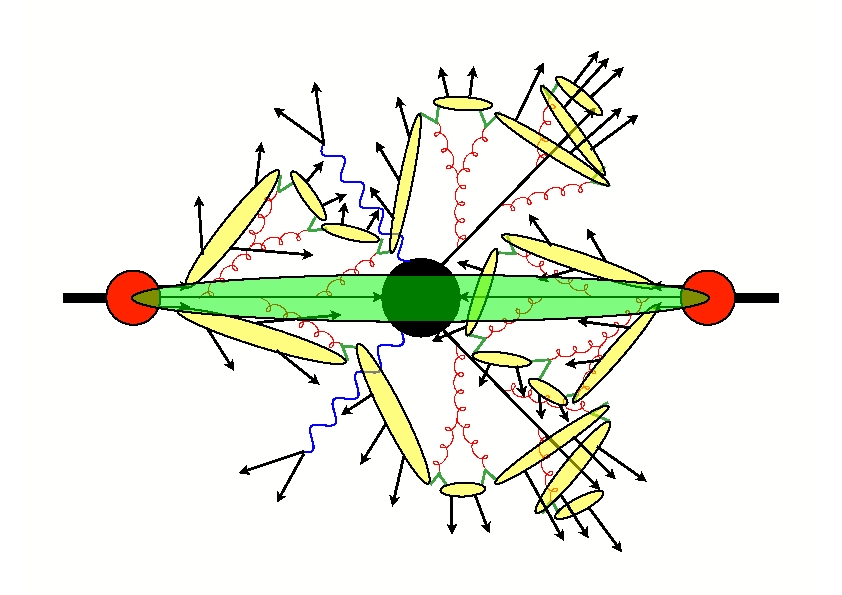
\includegraphics[width=\plotwidth]{figures/mc-schematic.jpg}
  }
  \caption[Two illustrations of a collision event]{Two illustrations of a collision event.  The first (reproduced from~\cite{Grogg:1376067}) is a simplified schematic showing the hard scattering interaction, parton shower, hadronization, and subsequent particle decays.  The second (reproduced from~\cite{Webber:2011}) gives a more complete picture with the hard scatter in green and the hadronization processes in yellow.}
  \label{diagram-showering}
\end{figure*}

\section{Underlying Event}

In addition to the parton showers originating from the hard interaction and from partons radiated in the initial or final state, soft radiation from the remaining partons must also be considered for a full picture of the event.  Because the partons originally formed a colorless proton, this soft radiation will be necessarily connected to the hard partons via a color field, influencing the color and distribution of new $q\bar{q}$ pairs pulled from the vacuum in order to conserve color charge.  The result is a large number of low energy hadrons distributed between the proton remnant and the hard jets which resulted from the final state partons.  This additional activity, known as the \emph{underlying event}, can deposit significant energy in the detector and must be modeled at the hadronization step.

\section{Pileup Interactions}

At LHC luminosities, we are not given the luxury of considering single events independently.  With thousands of protons in each bunch, there are often dozens of collisions in a single crossing.  For simulated events, we copy this effect by superimposing some number of soft interaction events on top of each nominal event, following the interaction multiplicity distribution observed in the experimental data as shown in Fig.~\ref{fig:pileup}.

\begin{figure}
  \centering
  \includegraphics[width=\plotwidth]{matplotlib/pileup}
  \caption[Distribution of the reconstructed collision vertex multiplicity observed in the 2011 data]{Distribution of the reconstructed collision vertex multiplicity observed in the 2011 data, demonstrating the magnitude of pileup effects.}
  \label{fig:pileup}
\end{figure}


\section{Detector Simulation}

The simulation steps discussed to this point cover only the initial evolution of the system within the vacuum of the beampipe.  As stable or long-lived particles produced in the hard scattering and hadronization processes travel outward from the collision point, they begin to interact with the material of the detector.  A detailed description of the CMS detector and magnetic field is used as input to the \GEANTfour package~\cite{Agostinelli2003250,Allison1610988}, a software toolkit for simulating the passage of particles through matter.  The software simulates not only the decays of the particles as they propagate through various materials, but also the interaction of those particles with the material and the response of the detector to the presence of those particles.  From that response, we simulate signals in the electronics to generate raw data in the same format produced by the physical detector.  From this point on, both collision data and Monte Carlo simulated events can be run through the same reconstruction and analysis software, maximizing the validity of comparisons between them. 


\section{Samples Produced}
\label{sec:mc-samples}
For all Monte Carlo samples considered in this analysis, a matrix element generator is interfaced with \PYTHIA~\cite{PYTHIA} which handles hadronization and then to \TAUOLA~\cite{Was:2000st} which handles all tau decays.  The CMS collaboration handles sample generation centrally whenever possible as a means to ensure consistency in configuration.  Except for our \wprime signal, we use official samples which have been configured to match the beam energy, detector conditions, and luminosity distribution of the full sample of collision data taken in 2011.

\begin{table}
\centering
\newcommand{\mymass}[1]{\makebox[\widthof{0000}][r]{#1}}
\newcommand{\mysigma}[1]{\makebox[\widthof{\num{1.000e-1}}][l]{\num{#1}}}
\begin{tabular}{ c c c c }
  \toprule
  $M(\wprime)c^2/\GeV$ & $\sigma_\mathrm{LO}/\pb$ & $\sigma_\mathrm{NNLO}/\pb$ & $k$\\
  \midrule
  \mymass{ 200} & \mysigma{1.324e0 } & \mysigma{1.797e0 } & 1.357\\
  \mymass{ 250} & \mysigma{1.118e0 } & \mysigma{1.517e0 } & 1.357\\
  \mymass{ 300} & \mysigma{6.337e-1} & \mysigma{8.599e-1} & 1.357\\
  \mymass{ 400} & \mysigma{2.040e-1} & \mysigma{2.768e-1} & 1.357\\
  \mymass{ 500} & \mysigma{7.915e-2} & \mysigma{1.074e-1} & 1.357\\
  \mymass{ 600} & \mysigma{3.620e-2} & \mysigma{4.890e-2} & 1.351\\
  \mymass{ 700} & \mysigma{1.806e-2} & \mysigma{2.440e-2} & 1.352\\
  \mymass{ 800} & \mysigma{9.857e-3} & \mysigma{1.328e-2} & 1.347\\
  \mymass{ 900} & \mysigma{5.551e-3} & \mysigma{7.440e-3} & 1.341\\
  \mymass{1000} & \mysigma{3.322e-3} & \mysigma{4.420e-3} & 1.332\\
  \mymass{1100} & \mysigma{2.041e-3} & \mysigma{2.704e-3} & 1.325\\
  \mymass{1200} & \mysigma{1.289e-3} & \mysigma{1.690e-3} & 1.311\\
  \mymass{1300} & \mysigma{8.333e-4} & \mysigma{1.082e-4} & 1.298\\
  \mymass{1400} & \mysigma{5.395e-4} & \mysigma{6.900e-4} & 1.279\\
  \mymass{1500} & \mysigma{3.606e-4} & \mysigma{4.560e-4} & 1.265\\
  \bottomrule
\end{tabular}
\caption[Cross sections of \wprime{} signal samples]{An overview of the $W' \to WZ \to \ell\nu\ell\ell$ signal samples considered in this analysis, giving the \wprime mass along with the associated leading order (LO) and next-to-next-to-leading order (NNLO) cross sections in the SSM followed by the associated $k$-factor. These samples were locally produced, following the same prescription used for official samples.  The cross sections include the branching ratios for the bosonic decays into charged leptons ($e$, $\mu$, or $\tau$).}
\label{tab:signalsampleinfotable}
\end{table}

\begin{table}
\centering
\newcommand{\mysigma}[1]{\makebox[\widthof{\num{1.000e-1}}][l]{\num{#1}}}
\newcommand{\mubox}[1]{\makebox[\widthof{$\mu$}][c]{$#1$}}
\newcommand{\zzto}[2]{\ensuremath{ZZ \to \mubox{$#1$}^+ \mubox{$#1$}^- \mubox{$#2$}^+ \mubox{$#2$}^-}}
\begin{tabular}{ c r c c }
  \toprule
  & Sample & $\sigma_\mathrm{LO}/\pb$ & $\sigma_\mathrm{(N)NLO}/\pb$ \\
  \midrule
  \multirow{6}{\baselineskip}{\begin{sideways}\parbox{18mm}{\MADGRAPH}\end{sideways}}
  & $WZ(\to \ell\nu\ell\ell)\,+$ jets & \mysigma{7.19e-1} & \mysigma{8.79e-1} \\ 
  & $WW(\to \ell \nu \ell \nu)\,+$ jets & \mysigma{3.78e0} & \mysigma{4.89e0} \\
  & $Z(\to\ell\ell)\,+$ jets &  \mysigma{2.47e3} & \mysigma{3.05e3} \\ 
  & $W(\to\ell\nu)\,+$ jets & \mysigma{2.78e4} & \mysigma{3.13e4} \\ 
  & $V\gamma\, +$ jets & \mysigma{1.73e2} & ---  \\ 
  & $t\bar{t}\,+$ jets & \mysigma{9.48e1} & \mysigma{1.58e2} \\ 
  \midrule
  \multirow{6}{\baselineskip}{\begin{sideways}\parbox{15mm}{\POWHEG}\end{sideways}}
  & \zzto{$e$}{$e$} & --- & \mysigma{1.54e-2} \\
  & \zzto{$\mu$}{$\mu$} & --- & \mysigma{1.54e-2} \\
  & \zzto{$\tau$}{$\tau$} & --- & \mysigma{1.54e-2} \\
  & \zzto{$e$}{$\mu$} & --- & \mysigma{3.08e-2} \\
  & \zzto{$e$}{$\tau$} & --- & \mysigma{3.08e-2} \\
  & \zzto{$\mu$}{$\tau$} & --- & \mysigma{3.08e-2} \\
  \bottomrule
\end{tabular}
\caption[Cross sections of background samples]{Background processes considered for this analysis with leading order (LO) and higher-order cross sections.  Each process corresponds to a dataset from official production, using either \MADGRAPH or \PYTHIA for the matrix element calculation. The $W\,+$ jets cross section is next-to-next-to-leading order (NNLO) while all others are next-to-leading order (NLO).  The $V\gamma\,+$ jets sample considers both of the heavy vector ($V$) bosons $W$ and $Z$.}
\label{tab:sampleinfotable}
\end{table}

\subsection{Backgrounds}
All simulated background samples are taken from official production of Monte Carlo events (see Table~\ref{tab:sampleinfotable}).  The matrix element calculation is handled by either \MADGRAPH~\cite{MADGRAPH} or \POWHEG~\cite{POWHEG}, both programs which operate to fixed order in $\alpha_\text{s}$, generating a given electroweak final state with additional jets.  Where possible, we replace this fixed-order cross section with a value obtained from a higher-order calculation using a generator or dedicated program within the same phase space and parameters.

Our primary background for a resonant search is SM $WZ$ production.  The $WZ$ Monte Carlo events are generated with \MADGRAPH while the cross section is taken from MCFM~\cite{Campbell:2011bn}.  We must also consider $ZZ$ production as an irreducible background where one of the leptons is either outside detector acceptance or is misreconstructed.  The other backgrounds represent reducible processes that can be confused with signal due to misidentified lepton candidates from jets and photons.  We expect these events with jets faking leptons to be a significant concern, so we pay special attention that the jets are well-modeled in the Monte Carlo.  \MADGRAPH is designed with such needs in mind and includes diagrams with up to four jets in addition to the base process for which it is configured.  This treatment, coupled with an accurate model of parton showering and the detector's response to jet activity, allows CMS to model the probability that jets are misreconstructed as charged leptons.

\subsection{Signal}
Both \wprime and Technicolor models are implemented in the current version of \PYTHIA.  The current implementation of LSTC which corresponds to the Technicolor parameter space of interest for this study, however, contains errors leading to an artificially low fraction of longitudinally polarized technihadrons.  Because the expected kinematics for \technirho{} events in the LSTC are quite similar to those for SSM \wprime, the \PYTHIA \wprime routines can also serve as a sufficient model for Technicolor events.  

Although \PYTHIA considers only leading order diagrams in its matrix element calculations, we can apply a scaling factor to the results in order to bring the overall cross section in line with a higher-order calculation.  For all signal samples, we employ an NNLO calculation from MCFM which includes all diagrams of order $\alpha_\text{s}$ as well as the ``box diagram'' for $WZ$ radiation initiated from a pair of gluons, which is of order $\alpha_\text{s}^2$.

For the \wprime search, we focus on fifteen individual mass points between \simass{200} and \simass{1500}, in each case producing \num{20000} events in \PYTHIA and an NNLO cross section in MCFM
(see Table~\ref{tab:signalsampleinfotable}).  
For Technicolor investigations, we use these same \wprime samples from \PYTHIA, but apply modified cross sections.  Each sample is assigned a leading order cross section from the \PYTHIA LSTC implementation which is then scaled by a factor $\sigma_\text{NNLO}/\sigma_\text{LO}$ (known as a $k$-factor) determined from the MCFM calculations for \wprime (see Table~\ref{tab:technicolorgen}).

% COMMENT:
% Technically NLO means including diagrams for process with the same 
% final states that take place at higher order due to loops.
% Commonly in the field NLO means including diagrams with the same electroweak
% final state particles and additional jets due to QCD radiation.  When your read
% about an NNLO cross section predictions for WZ production what they are
% really talking about is including final states with up to two jets.   
% The order they are talking about is actually the order of the strong
% coupling constant beyond the order in alpha_s necessary to produce the
% basic electroweak final state.  Also often included in an NNLO calculation 
% will also be loop diagrams to the same order in alpha_s.  So for WZ production
% an NNLO calculation would include WZ, WZ+1jet, WZ+2jets, WZ produced via
% gluons to a box diagram(two strong vertices) with the WZ radiated off of
% the other side of the box.  Note that sometimes the last is not included
% because it is technically very difficult.  Sometimes they will include
% diagrams with extra electroweak couplings, but typically not because
% every electroweak vertex has an on order 1/137 suppression and the
% addition to the cross section is small.  Also sometimes a cross section
% calculation will include an attempt to resum all higher order effects
% (resummation) after the NNLO treatment to improve the final result.  That
% is why you would want to normalize to that number to improve the result.


\begin{table*}[!h]
  \centering
  \begin{tabular}{c c c c c c}
    \toprule
    $M(\technirho)$ & $M(\technia)$ & $M(\technipi)$ & $(\sigma_\text{LO} \times \text{BR})/\pb$ & $(\sigma_\text{NNLO} \times \text{BR})/\pb$ \\
    \midrule
    200 & 220 & 125 & \num{3.872e-1} & \num{5.254e-1} \\ %            
    250 & 275 & 163 & \num{2.144e-1} & \num{2.909e-1} \\ %            
    300 & 330 & 200 & \num{9.616e-2} & \num{1.305e-1} \\ %\num{42.74} 
    400 & 440 & 275 & \num{2.889e-2} & \num{3.920e-2} \\ %\num{12.84} 
    500 & 550 & 350 & \num{1.172e-2} & \num{1.590e-2} \\ %\num{5.208} 
    600 & 660 & 425 & \num{5.612e-3} & \num{7.582e-2} \\ %\num{2.494} 
    700 & 770 & 500 & \num{2.943e-3} & \num{3.979e-3} \\ %\num{1.308} 
    800 & 880 & 575 & \num{1.670e-3} & \num{2.249e-3} \\ %\num{0.742} 
    900 & 990 & 650 & \num{9.740e-4} & \num{1.306e-3} \\ %\num{0.432} 
    \bottomrule
  \end{tabular}
  \caption[Technicolor parameters used for cross section generation]{Technicolor parameters used to generate cross sections for this analysis.  All masses are given in \GeVcc.  BR refers to the product of the branching ratios of the \technirho/\technia to $WZ$ and the subsequent decay of $W$ and $Z$ to electrons, muons, or taus.  Quoted cross sections are computed by \PYTHIA to leading order (LO).}
  \label{tab:technicolorgen}
\end{table*}

For Technicolor, we concentrate on the TCSM mass points not excluded by other experiments which cover a phase space region accessible with \SI{5}{\fbinv} of data.  As discussed in Section~\ref{sec:technicolor}, suppression of the electroweak $S$ parameter requires near degeneracy between the vector and axial-vector resonances; we choose $M(\technia) = 1.1 M(\technirho)$.

The relationship between $M(\technirho)$ and $M(\technia)$ significantly affects $\text{BR}(\technirho \to WZ)$.  The $WZ$ branching ratio drops below 10\% for $M(\technirho) > M(\technipi)$, but approaches unity if $M(\technirho) < M(\technipi) + M(W)$.  For this analysis, we assume a parameter set used in previous CMS investigations~\cite{Brooijmans:2010tn} where $M(\technipi) = \frac{3}{4} M(\technirho) - 25\GeV$ and also investigate the dependence of the results on the relative values of the \technirho and \technipi masses.
\resetlinenumber
% \chapter{Event Reconstruction}
\label{chapter:reconstruction}

The Compact Muon Solenoid, comprised of millions of individual detector channels, cannot by itself give us information about what particles have traveled through its volume; it can only offer a readout of hits in the muon and tracking detectors, energy deposits in the calorimeters, and other basic electronic signals.  The trajectories and identities of the particles which induced that detector response must be inferred through reconstruction algorithms which draw on the raw detector data to build a more coherent picture of a collision event.  The success of this analysis thus rests both on the successful functioning of the detector hardware and on the logic which builds electrons, muons, and \MET from the hardware output.  An initial view of such reconstructed output can be seen in Fig.~\ref{fig:visualization} which visualizes the content of a recorded $WZ$ event.

\begin{figure*}
  \centering
  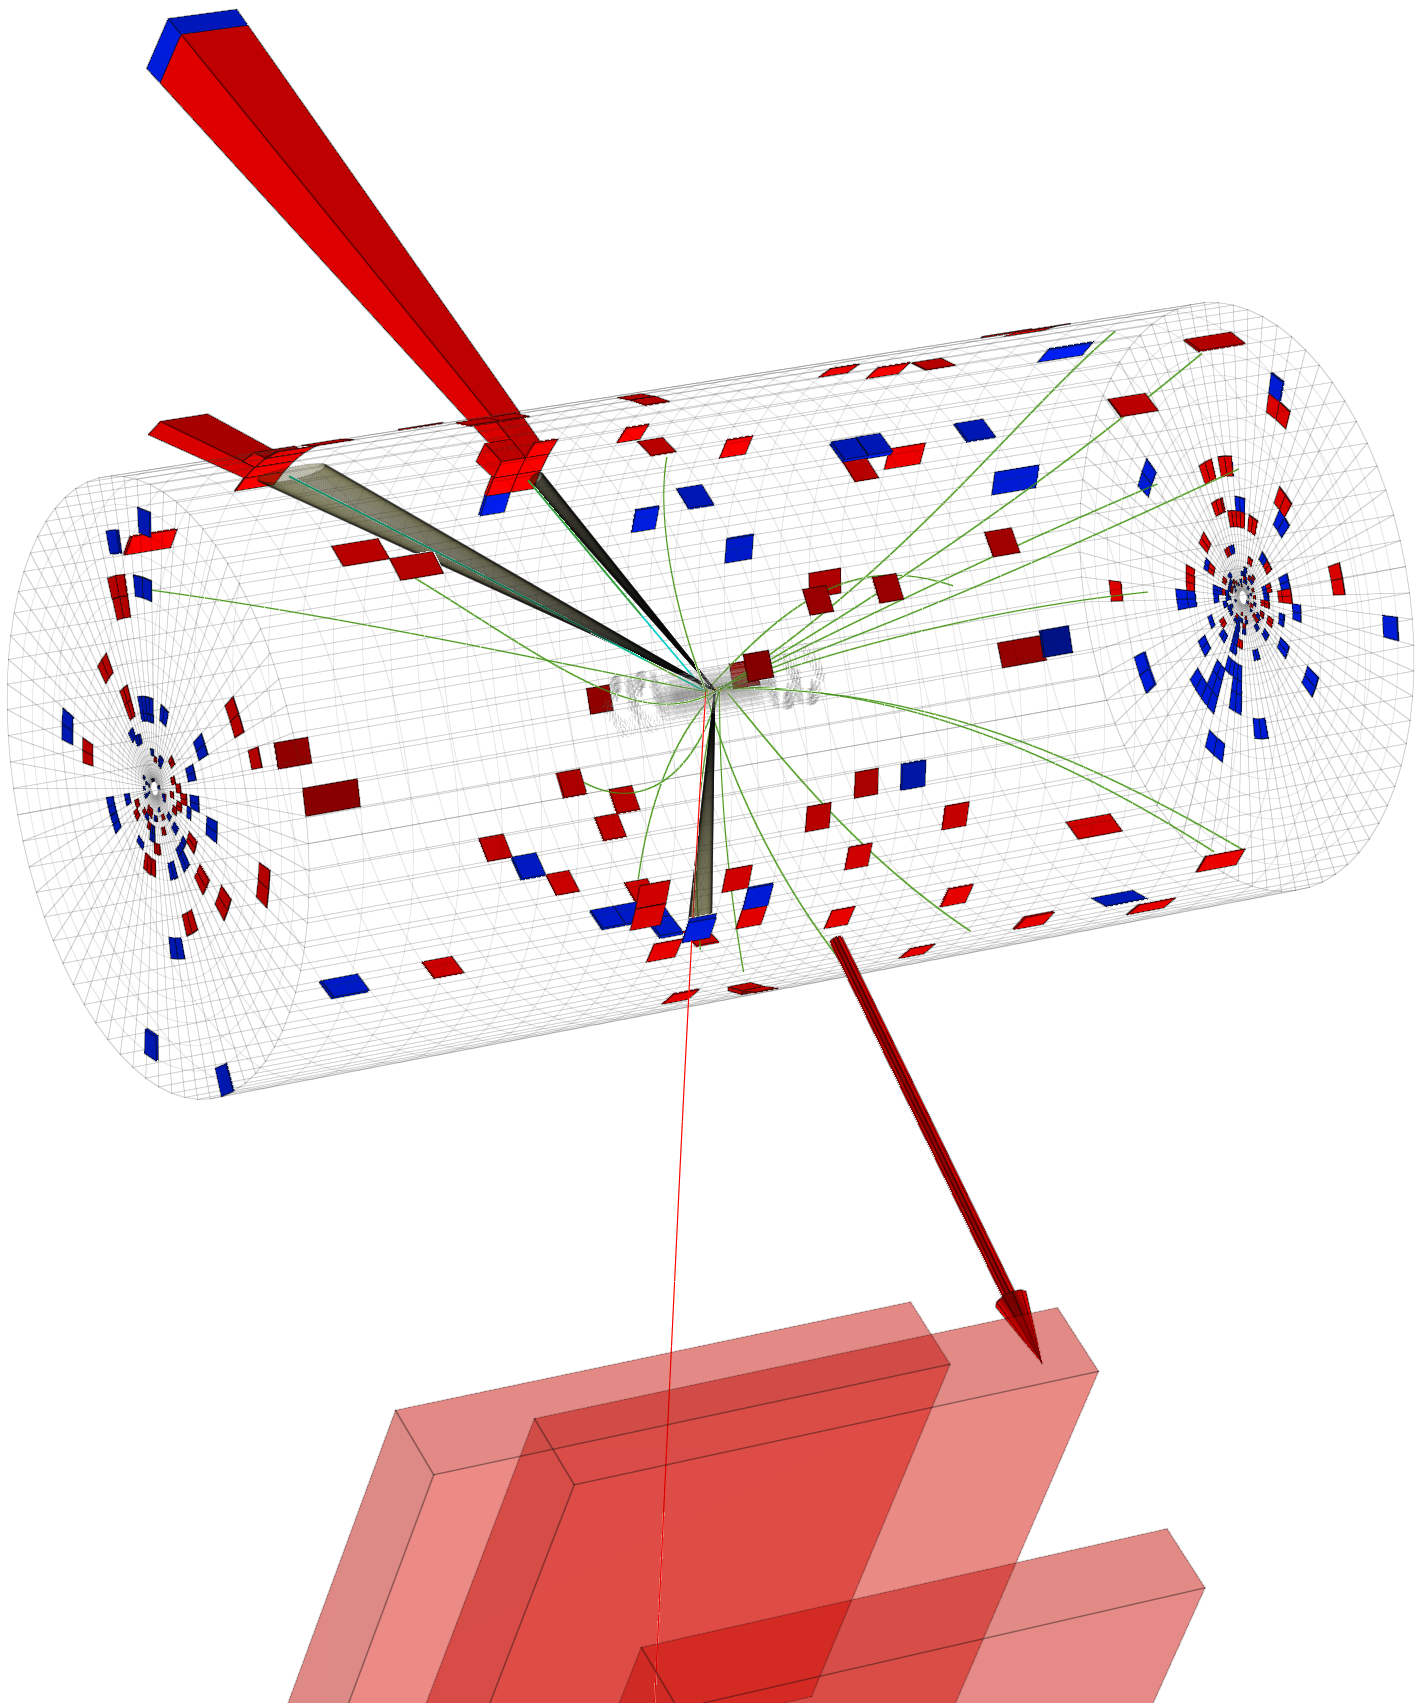
\includegraphics[width=\plotwidth]{figures/167103.79.73561307.png}
  \caption[Visualization of a $WZ$ event in CMS]{Visualization of a $WZ$ event in CMS (Run 167103, Event 73561307, recorded Friday, 17 June 2011).  The wireframe shows the volume of the inner tracker, with generic reconstructed tracks drawn in green.  The heights of red and blue columns resting on the wireframe surface indicate the magnitudes of energy deposits in the \ecal and \hcal respectively.  The $Z$ boson has decayed into two electrons, emerging from the far side of the tracker; they appear as light blue tracks accompanied by large \ecal deposits.  The $W$ boson has decayed into a muon and a neutrino (indicated by the large \MET arrow) in the foreground; the muon track is shown in red, extending outward to the muon chambers (shown as translucent red blocks).}
  \label{fig:visualization}
\end{figure*}


\section{Electron Reconstruction}

\begin{figure*}
  \centering
  \subbottom[An electron passing through the tracker, then depositing energy in the \ecal{} crystals.  Note the distinct energy cluster due to a \brem{} photon.]{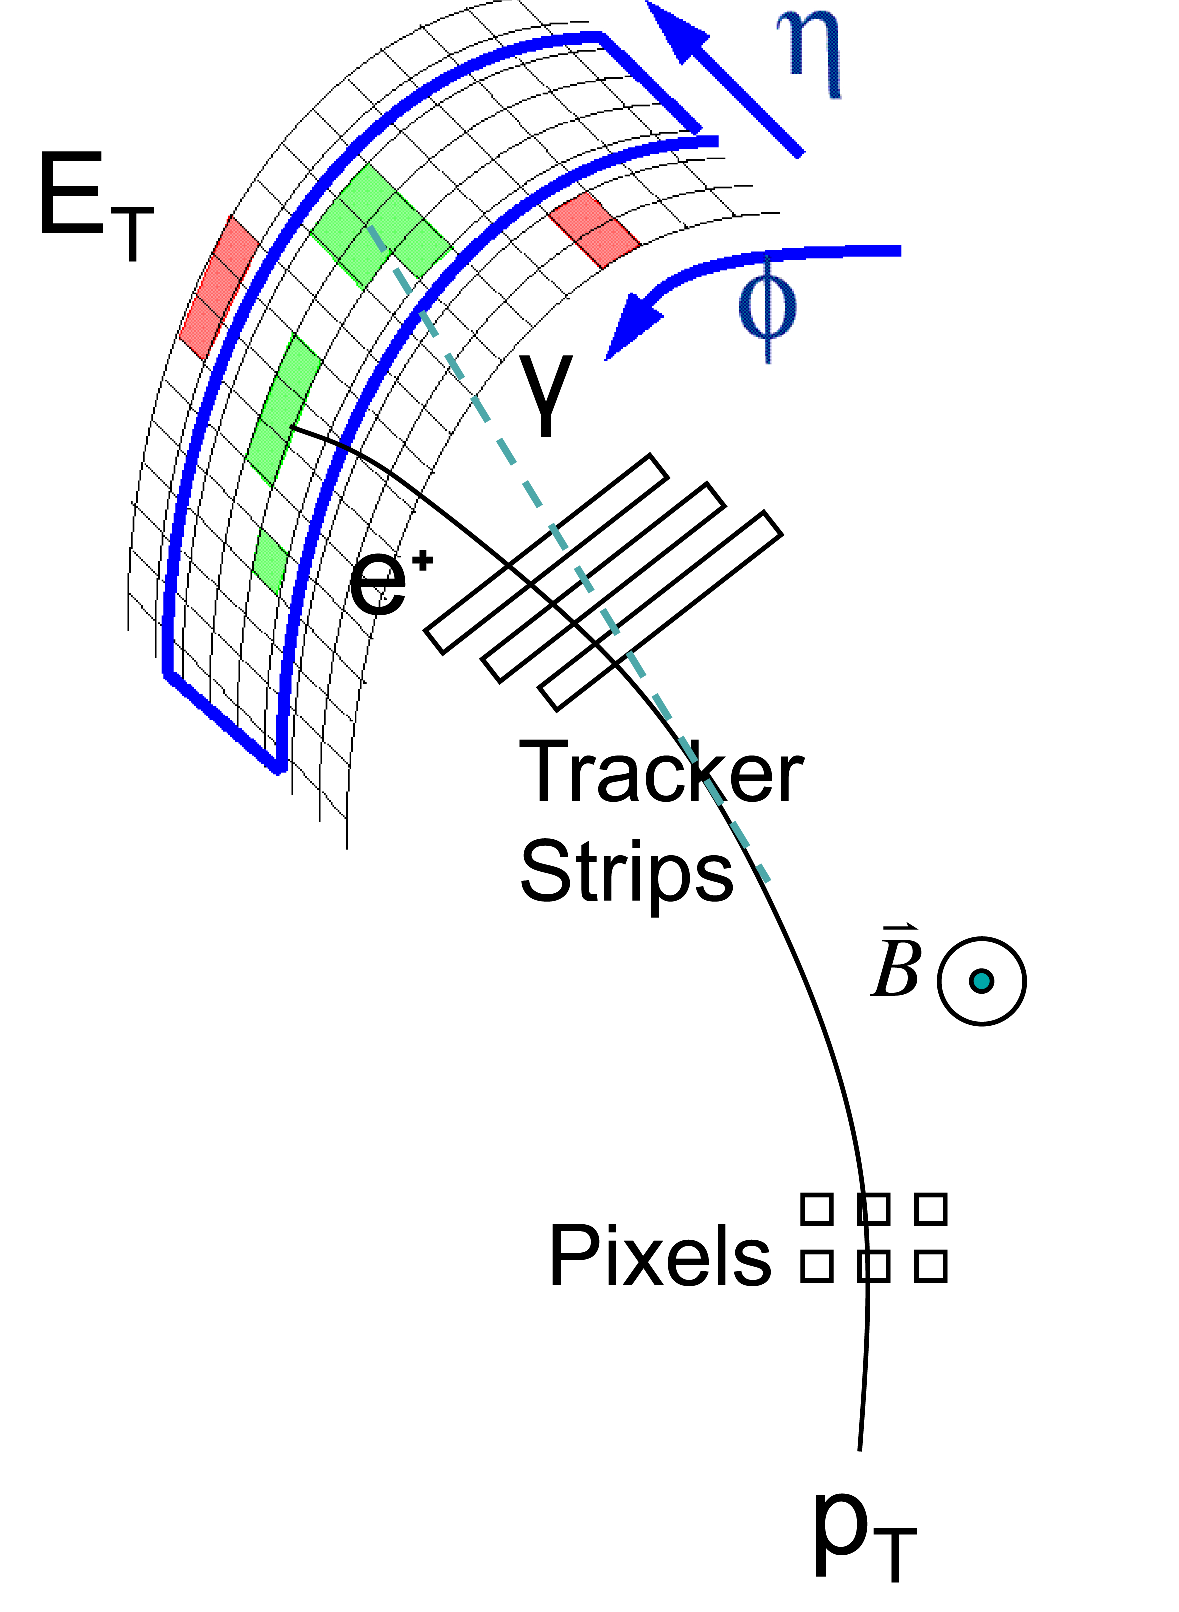
\includegraphics[width=0.47\textwidth]{figures/cms-electron-reco}\label{fig:cms-electron-reco}}
  \hfill
  \subbottom[Transverse event display showing the coincidence of a high-momentum track and a significant deposit of energy in the \ecal{} characteristic of an electron.]{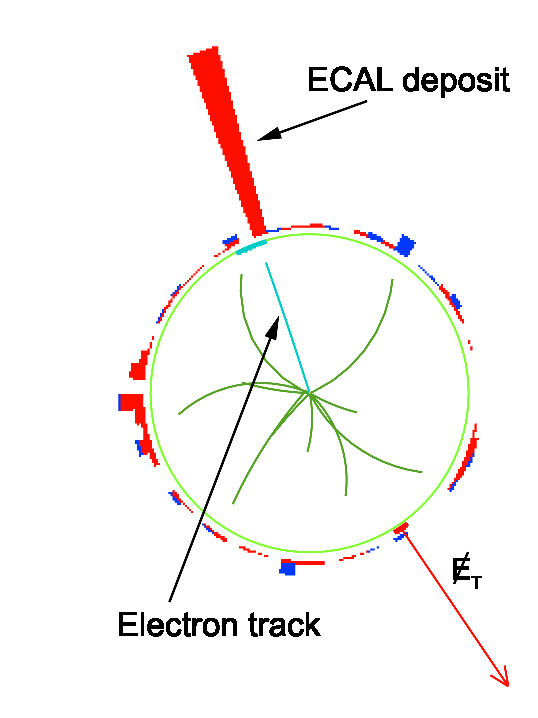
\includegraphics[width=0.47\textwidth]{figures/cms-electron-display}\label{fig:cms-electron-display}}
  \caption{Two diagrams showing the response of the CMS detector to a high-energy electron.}
  \label{fig:cms-electron-diagrams}
\end{figure*}

The basic signature for an electron in CMS is an ECAL energy deposit matched to a track in the inner tracker, which the CMS reconstruction software identifies via two complementary algorithms~\cite{CMS-PAS-EGM-10-004}.  The ``tracker-driven'' algorithm is optimized for low-\pt electrons and those inside jets, starting from a collection of tracks and looking for corresponding clusters of energy in the \ecal.  The ``\ecal-driven'' algorithm, however, is more relevant to this analysis since it is optimized for isolated electrons in the \pt range under consideration (\pt > 10).  As implied by its name, this technique starts in the \ecal, grouping together associated clusters of energy into ``superclusters'' which are narrow in $\eta$ but may have a significant spread in $\phi$, characteristic of an electron bending in the magnetic field and radiating as it passes through the tracker material.  Once these superclusters are identified, they are matched not with reconstructed tracks, but rather with pairs or triplets of hits in the innermost layers of the tracker.  These hits are used as seeds for a special electron tracking algorithm which takes into account a model of the typical electron energy loss when moving through the tracker.

At this reconstruction stage, some loose quality requirements are imposed to remove faulty candidates while maintaining an efficiency above 99\% for isolated electrons.  The ratio of energy deposited in the \hcal vs. the \ecal in the supercluster region must fall below 0.15 as significant deposits in the \hcal would indicate hadronic activity from a jet.  In addition, the displacement between the supercluster centroid and its associated track must fall within the bounds $\Delta\eta < 0.02$ and $\Delta\phi < 0.15$.  In general, the requirements imposed at the analysis level are more strict and supersede these reconstruction-level criteria.  Additionally, these requirements are loose enough that the objects classified as reconstructed electron candidates can be used to study other physics objects being misidentified as electrons.  The electron four-momentum and point of origin are assigned based on the track parameters at the distance of closest approach to the nominal beam spot, with the energy determined from a combination of tracker and \ecal information.


\section{Muon Reconstruction}
Muon reconstruction in CMS starts from local pattern recognition in each of the muon subsystems, followed by ``stand-alone'' and ``global'' reconstruction algorithms~\cite{CMS-MuonReco}.  The stand-alone reconstruction phase integrates information throughout the muon subsystems, linking together track segments from the individual chambers and fitting them into stand-alone muon tracks.  This algorithm looks for seeds in the innermost chambers, first building tracks outward using a Kalman-fitter technique~\cite{Fruhwirth1987444}, then refitting inward to define track parameters at the innermost muon station.  These stand-alone muons are then compared to independently-reconstructed tracks from the inner tracker by propagating those tracks to the inside surface of the muon detector.  Compatibility in terms of momentum, position, and direction are considered in matching stand-alone muons to tracker tracks and the hits from matched pairs are used as input for a new, global fit.  The resulting collection of global muon tracks may contain ambiguities and poor matches, so arbitration and quality algorithms are applied to choose at most one final global track to associate with each stand-alone muon.

While the inner tracker can in general provide a much higher momentum resolution than the muon system due to its high granularity and the greater multiplicity of hits available for the track fit, the combination of these two systems becomes important for muons with momentum above \simomentum{100}.  At high energies, the reduced bending of the muon tracks limits the resolution of the inner tracking algorithms.  In these cases, just a few hits at the large radius of the muon system can significantly improve the curvature measurement, constraining the fit and providing a better momentum resolution.  A high-quality muon is expected to have at least one hit within the muon chambers and at least one within the inner pixel tracker, with a greater multiplicity of hits generally correlated with a better-reconstructed track.  The quality of the fit is estimated through a normalized $\chi^2$ determination.  Prompt muons can be distinguished from secondary muons produced in hadronic decays through measurement of the impact parameter of the track with respect to the primary vertex.

As an alterative to stand-alone and global muons, CMS employs an algorithm for identifying ``tracker muons'' which consist of tracks in the inner tracker matched to individual muon segments.  In this scenario, all tracks with $\pt > \simomentum{0.5}$ and total momentum $p > \simomentum{2.5}$ act as seeds and are considered as muon candidates if they can be matched to at least one muon segment.  While this approach can be particularly useful for low-\pt studies where the global reconstruction algorithm degrades, it maintains a high efficiency over the entire muon \pt range.  For this analysis, we use this tracker-driven algorithm as a cross-check for muon quality; all global muons considered in the analysis must also be identified as tracker muons.

\section{Jet Reconstruction}
\label{sec:jet-reco}

While both electron and muon reconstruction algorithms are able to use the high granularity of the tracker as a clear guide towards deposits elsewhere in the detector, jets are partially composed of neutral particles which do not leave tracks, necessitating a significant reliance on the calorimeters.  As a result, a direct search for jets introduces ambiguity which limits the effectiveness of reconstruction algorithms.  This difficulty motivates the CMS particle flow algorithm~\cite{ParticleFlow} which seeks to provide a more nuanced view of an event by reconstructing physics objects in sequence, removing tracker hits and energy deposits from consideration once they are assigned to a particular object.  In this approach, muons are reconstructed first, accounting for all segments in the muon chambers while removing related tracks in the tracker and energy deposits in the calorimeter before moving on to electrons and jets.  The input to the jet reconstruction algorithm, then, is a collection of energy deposits which have a high likelihood of belonging to a jet, allowing for a more efficient reconstruction.

Within the context of particle flow, jets are created by means of the ``anti-$k_\text{T}$'' clustering algorithm~\cite{antikt} which looks for a high-momentum particle as a seed, then adds nearby particles to the jet with weights corresponding to their momenta.  This algorithm is both ``infrared safe'' in the sense that it is not affected by the presence of the infinitely soft particles which result from QCD divergences and also ``collinear safe'' in the sense that it automatically recombines collinear partons~\cite{Ellis:1993tq}.  These two qualities are essential to allow meaningful comparisons between reconstructed jets and theoretical calculations to arbitrary order.  

\section{Pileup}
\label{sec:pileup}

The intense luminosity provided by the LHC creates an environment where each bunch crossing can lead to dozens of individual $pp$ collisions.  While the high resolution of the tracker allows association of charged particles to distinct vertices, the same technique cannot be used for neutral particles which leave no signature in the tracker.  For jet measurements in particular, the heavy reliance on calorimeters limits the ability to distinguish vertices.  In most events of interest, there is only one hard scattering interaction; the various other proton collisions, known as \emph{pileup}, are typically soft, leading to significant jet activity, particularly in the forward regions of the detector.  The number of pileup interactions in a given bunch crossing has a significant effect on our resolution for jet energy measurements, motivating an event-by-event treatment to correct for these effects.

One of the major treatments for this type of pileup correction at CMS is the \textsc{fastjet} algorithm~\cite{Cacciari:2007fd,Cacciari:2008gn} which estimates an energy contribution due to pileup for each reconstructed jet which can then be subtracted from the jet's energy to yield a result which more closely represents the energy of the initiating parton.  The algorithm proceeds by assigning an abstract ``area'' $A$ to each jet which is essentially a measurement of its susceptibility to pileup contamination while measuring the overall level of diffuse noise $\rho$ in the event as the median value of $\pt/A$ taken over all jets.  In the analysis given here, the \textsc{fastjet} algorithm will be important for applying pileup corrections to the isolation sums considered for identification of leptons (see Secs.~\ref{sec:electron-selection} and~\ref{sec:muon-selection}).

\section{Missing Transverse Energy}
\label{sec:met}

Although the neutrino produced in a $W \to \ell \nu$ decay will leave no deposits within the detector, we can use the visible particles in the event and the principle of momentum conservation to infer its presence.  Although the center of momentum in a hard interaction at the LHC may carry a significant longitudinal boost with respect to the lab frame, the interacting partons should have negligible momentum transverse to the beampipe.  The vector sum of the transverse momenta of the decay products, therefore, should be very small in magnitude, and any significant imbalance would indicate the direction and momentum of a particle which escaped the detector without interacting.

Such an imbalance is traditionally known as missing transverse energy (\MET), with the measurement relying on calorimetric information.  The hermetic coverage of the CMS calorimeters lends itself well to this kind of measurement, and indeed the CMS reconstruction software defines a calorimeter-based \MET vector:
\begin{equation}
  \vecMET \equiv - \sum_{i} \vec{E}_\text{T}(i),
\end{equation}
where $i$ iterates over all energy deposits in the calorimeters and $\vec{E}_\text{T}(i)$ is the transverse projection of a vector with magnitude equal to the selected energy deposit, pointing from the interaction region toward the deposit.

This relatively simple definition of \MET, however, does not fully exercise the capabilities of the CMS detector since it ignores the various tracking systems and makes no effort to match the energy deposits to any particle hypothesis which might help distinguish their origin.  As with jet reconstruction, significant resolution can be gained for \MET by taking a particle flow approach.

Within the context of particle flow, missing transverse energy can be calculated from the vector sum of the transverse momenta for all reconstructed particles:
\begin{equation}
  \vecMET \equiv - c \sum_{i} \vec{p}_\text{T}(i),
\end{equation}
where $i$ iterates over all objects identified by the particle flow algorithm.  For the present analysis, we prefer the dedicated electron and muon reconstruction algorithms over particle flow due to their comparative simplicity, but the particle flow definition of \MET has been shown to have good reliability and significantly enhanced resolution with respect to the traditional calorimetric definition and is thus suitable for use here.

\resetlinenumber
% \chapter{Event Selection}
\label{chapter:selection}

The \wztolnll{} decay is characterized by:
\begin{itemize}
\item a pair of same-flavor, opposite-charge, high-\pt, isolated leptons with an invariant mass consistent with a $Z$ boson,
\item a third high-\pt, isolated lepton, and
\item a significant deficit of transverse energy (\MET) associated with the escaping neutrino.
\end{itemize}
The selection criteria used for this analysis aim to identify $WZ$ events with as high an efficiency as possible while rejecting a significant fraction of background events with similar signatures.  The above characteristics can be supplemented by requirements related to the overall energy scale of the interaction for cases where the the $WZ$ pair originates from a massive resonance.  These criteria will be applied both to a measurement of the cross-section for SM $WZ$ production and to a search for a resonance in the $WZ$ spectrum, so there are certain places where the criteria diverge to provide optimal performance in different contexts, but the majority of the selection is uniform between the two measurements.

\section{Online Event Selection}
Over the course of 2011, CMS recorded \recordedlumi{} of $pp$ collision data, broken up into two major periods separated by a short technical stop.  
Each of the subsystems of the CMS detector experiences some amount of downtime due to equipment failures, meaning that some fraction of the recorded luminosity cannot be used for general analyses which rely on the integration of the full detector.  Consequently, the collaboration certifies a list of runs suitable for physics publication, which in the case of the 2011 data is equivalent to \jsonlumi.

Because the LHC delivers many more collisions than the CMS detector can record, the trigger system steps in to make quick decisions on which are worth keeping and which will not be as interesting for analysis.  The various triggers target different physics objects; among the many triggers available, one requires a single high-\pt electron, another requires a pair of electrons of intermediate \pt, and likewise for muons.  Since the events firing each type of trigger are generally independent, the data is naturally sorted into primary datasets (PDs) based on trigger type.

These primary datasets (and indeed the entire set of recorded data) are necessarily biased in favor of events with certain content.  This bias has potential repercussions for physics results and must be considered when constructing an analysis.  To ensure a sufficient understanding of the online selection, some portion of each analysis effort goes into carefully measuring the efficiency for events of interest to fire the relevant triggers and incorporating that information into the final result.  Often, this means not only choosing some small number of datasets for the selection of signal events, but also an additional set with different biases to allow the efficiency measurements.

For this analysis, we consider the \texttt{DoubleElectron} and \texttt{DoubleMu} datasets where events must fire a trigger looking for a pair of electrons or a pair of muons, respectively.  To control the recorded event rate, each of these triggers imposes energy thresholds on the candidate objects, with these thresholds increasing as the luminosity has increased.  These HLT paths are each seeded by a Level-1 trigger path requiring one or two low-level detector objects with thresholds lower than those imposed at higher levels.  The thresholds corresponding to various run ranges are given in Table~\ref{tab:trigger-thresholds}.

\begin{table}
  \centering
  \begin{tabular}{c r r r r r r r r}
    \toprule
    % & \multicolumn{8}{c}{Thresholds/\GeV} \\ \cmidrule{2-9}
    & \multicolumn{4}{c}{$\et(e^\pm)$/(\GeV)} & \multicolumn{4}{c}{$\pt(\mu^\pm)$/(\GeVc)} \\ \cmidrule(r){2-5} \cmidrule(l){6-9}
    Run Range & \multicolumn{2}{c}{L1} & \multicolumn{2}{c}{HLT} & \multicolumn{2}{c}{L1} & \multicolumn{2}{c}{HLT} \\ 
    %\midrule
    \cmidrule(r){1-1} \cmidrule(rl){2-3} \cmidrule(rl){4-5} \cmidrule(rl){6-7} \cmidrule(l){8-9}
    160329--164236 & 12 & --- & 17 & 8 & 3 & 3 &  7 & 7 \\
    165088--170759 & 12 & --- & 17 & 8 & 3 & 3 & 13 & 8 \\
    170826--178380 & 12 &   5 & 17 & 8 & 3 & 3 & 13 & 8 \\
    178420--180296 & 12 &   5 & 17 & 8 & 3 & 3 & 17 & 8 \\
    \bottomrule
  \end{tabular}
  \caption[Trigger thresholds]{Thresholds for the double electron and double muon triggers used in this analysis.  The Level-1 seed for the electron triggers initially requires only one object with $\et > \sienergy{12}$, but later requires an additional deposit with $\et > \sienergy{5}$.}
  \label{tab:trigger-thresholds}
\end{table}

\section{Electron Selection}
\label{sec:electron-selection}
Although previous experiments have developed multivariate discriminators to provide optimal efficiency in identifying high-quality electrons, this analysis chooses a simpler cut-based approach.  This choice reflects both the necessity to build understanding of lepton identification during the first year of full LHC operation and the excellence of the CMS detector that in most analyses makes complicated multivariate lepton identification unnecessary.  We define a separate set of requirements for each of the three lepton roles, with the requirements on an electron associated with the $W$ significantly tighter than those for the $Z$ leptons.  Whereas the invariant mass constraint on the $Z$ leads to a relatively pure sample of $Z$ bosons, there is a high probability to choose a jet when searching for a $W \to e + \nu$ decay.  The selection criteria are specifically chosen to reduce the frequency of jets entering into the pool of electron candidates.

Electrons assigned to a $Z$ decay are required to match objects passing the double electron trigger.  The matching compares the $(\eta, \phi)$ coordinates of the reconstructed electrons and the electron objects identified in the HLT, requiring $\Delta R < 0.1$ (see Eq.~\ref{eq:deltar}).  In order to ensure a high trigger efficiency, we must impose \et requirements on the reconstructed electrons such that they lie on the plateau of the trigger efficiency curve with respect to electron \et.  To match the trigger thresholds of \sienergy{17} and \sienergy{8}, the leading electron must have $\et > \sienergy{20}$ while the other may have \et as low as \sienergy{10}.

All electrons must be within the detector acceptance ($|\eta| < 2.5$) and meet several criteria testing the compatibility of the electromagnetic shower shape with the isolated electron hypothesis.  The shower is evaluated for the width of the electromagnetic cluster in terms of pseudorapidity ($\sigma_{i\eta i\eta}$ where $i$ indicates that the measurement is taken as a number of crystals rather than a distance, see Sec.~\ref{sec:ecal}), the difference in the measured position of the \ecal supercluster vs.\ the associated track ($\Delta\phi$ and $\Delta\eta$), and the ratio of energy deposited in the \ecal vs.\ the \hcal ($E_\text{HCAL} / E_\text{ECAL}$).  Because calorimeter response differs significantly between the barrel and the endcap, the values for these criteria are determined separately for these two regions.  Table~\ref{tab:electron-requirements} gives the specific values for all electron requirements applied in this analysis with the corresponding distributions shown in Fig.~\ref{fig:electron-cuts-hb} for candidates in the barrel region and Fig.~\ref{fig:electron-cuts-he} for candidates in the endcap region.

\begin{table*}
  \centering
  \begin{tabular}{rrrrrrr}
    \toprule
    & \multicolumn{2}{c}{Electrons from $Z$} & \multicolumn{2}{c}{Electron from $W$} \\ \cmidrule(r){2-3} \cmidrule(l){4-5}
    Requirement & EB & EE & EB & EE \\
    \midrule
    Minimum trigger match \et (\GeV) & 17 (8) & 17 (8) & --- & --- \\
    Minimum electron \pt (\GeVc) & 20 (10) & 20 (10) & 20 & 20 \\
    Maximum $\sigma_{i\eta i\eta}$ & 0.012 & 0.031 & 0.010 & 0.031 \\
    Maximum $|\Delta\eta_\text{in}|$ & 0.007 & 0.011 & 0.005 & 0.006 \\
    Maximum $|\Delta\phi_\text{in}|$ & 0.800 & 0.700 & 0.027 & 0.021 \\
    Maximum missing track hits & 0 & 0 & 0 & 0 \\
    Minimum $d$ between tracks (\si{cm})& --- & --- & 0.02 & 0.02 \\
    Minimum $\Delta\cot(\theta)$ between tracks & --- & --- & 0.02 & 0.02 \\
    Maximum $R_\text{iso}$ & 0.15 & 0.10 & 0.07 & 0.06 \\
    Minimum $\Delta R$ from any muon & 0.01 & 0.01 & 0.01 & 0.01 \\
    \bottomrule
  \end{tabular}
  \caption[Requirements imposed on electrons]{Requirements imposed on electrons.  The first two rows give criteria applied to the more energetic $Z$ electron first, with the value for the less energetic electron in parentheses.}
  \label{tab:electron-requirements}
\end{table*}

\begin{figure*}[p]
  \centering
  \newcommand{\mywidth}{0.47\textwidth}
  \newcommand{\mygraph}[1]{\includegraphics[width=0.49\textwidth]{matplotlib/#1.\figext}}
  \mygraph{lepcuts100/hb_pt}\hfill\mygraph{lepcuts10/hb_iso}\\
  \mygraph{lepcuts100/hb_detain}\hfill\mygraph{lepcuts100/hb_dphiin}\\
  \mygraph{lepcuts100/hb_nmiss}\hfill\mygraph{lepcuts100/hb_sieie}\\
  \mygraph{lepcuts100/hb_dist}\hfill\mygraph{lepcuts100/hb_dcot}\\
  \caption[Distributions of criteria used to select barrel electrons]{Distributions of criteria used to select barrel electrons, considering all remaining candidates with $\et > \sienergy{20}$ after a \ztoll{} decay is identified.  Collision data (composed mostly of jets) is compared to simulated $WZ$ events (composed mostly of true electrons) to show the discriminating power of each requirement.  Shaded areas indicate excluded regions; when two different depths of shading are used, the lighter one indicates a region of conditional exclusion as described in Table~\ref{tab:electron-requirements}.}
  \label{fig:electron-cuts-hb}
\end{figure*}

\begin{figure*}[p]
  \centering
  \newcommand{\mywidth}{0.47\textwidth}
  \newcommand{\mygraph}[1]{\includegraphics[width=0.49\textwidth]{matplotlib/#1.\figext}}
  \mygraph{lepcuts100/he_pt}\hfill\mygraph{lepcuts10/he_iso}\\
  \mygraph{lepcuts100/he_detain}\hfill\mygraph{lepcuts100/he_dphiin}\\
  \mygraph{lepcuts100/he_nmiss}\hfill\mygraph{lepcuts100/he_sieie}\\
  \mygraph{lepcuts100/he_dist}\hfill\mygraph{lepcuts100/he_dcot}\\
  \caption[Distributions of criteria used to select endcap electrons]{Distributions of criteria used to select endcap electrons, considering all remaining candidates with $\et > \sienergy{20}$ after a \ztoll{} decay is identified.  Collision data (composed mostly of jets) is compared to simulated $WZ$ events (composed mostly of true electrons) to show the discriminating power of each requirement.  Shaded areas indicate excluded regions; when two different depths of shading are used, the lighter one indicates a region of conditional exclusion as described in Table~\ref{tab:electron-requirements}.}
  \label{fig:electron-cuts-he}
\end{figure*}

Photons originating from a hard interaction have a high probability to convert to an $e^+e^-$ pair within the tracker.  Those tracks, however, are likely to be missing hits in the innermost regions, so we can discriminate against them by requiring that electron tracks have no missing hits.  Electrons assigned to a $W$ decay are also checked for extra tracks in their immediate vicinity and rejected if any fall within a distance $d$ of \SI{0.2}{mm} or are not sufficiently separated to satisfy $\Delta\cot(\theta) < 0.02$.

For isolation, we take the approach of drawing a cone (defined as $\Delta R < 0.3$) around each electron and looking for objects inside that cone.  The objects considered include tracks in the inner tracker where the cone is defined around the electron track's position from the origin as well as calorimeter deposits where the cone is defined around the electron's location at the inside surface of the \ecal.  Isolation is quantified as a sum of the transverse energies of all tracks and calorimeter deposits within those cones which are not associated with the electron:
\begin{equation}
  \label{eq:isolation}
  \et^\text{iso} = c \cdot \!\!\!\sum_i^\text{tracker}\!\!\! \pt(i) + \!\!\!\sum_i^\text{ECAL}\!\!\! \et(i) + \!\!\!\sum_i^\text{HCAL}\!\!\! \et(i).
\end{equation}
In order to allow a high acceptance for energetic electrons, we set a requirement not on the isolation sum itself, but rather on the ratio of the isolation sum to the electron's transverse momentum:
\begin{equation}
  \label{eq:riso}
  R_\text{iso} = \frac{\et^\text{iso}}{c \cdot \pt}.
\end{equation}

\begin{figure*}[!htbp]
  \centering
  \subbottom[Before correction.]{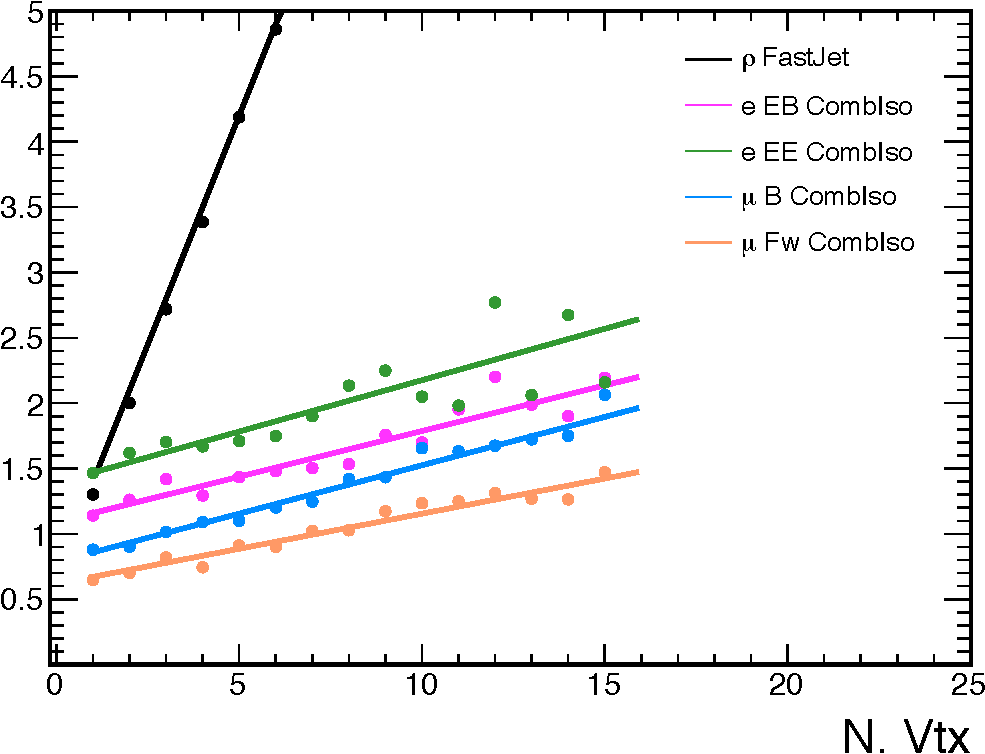
\includegraphics[width=0.47\textwidth]{figures/fastjet-before-crop}\label{fig:fastjet-before}}
  \hfill
  \subbottom[With correction applied.]{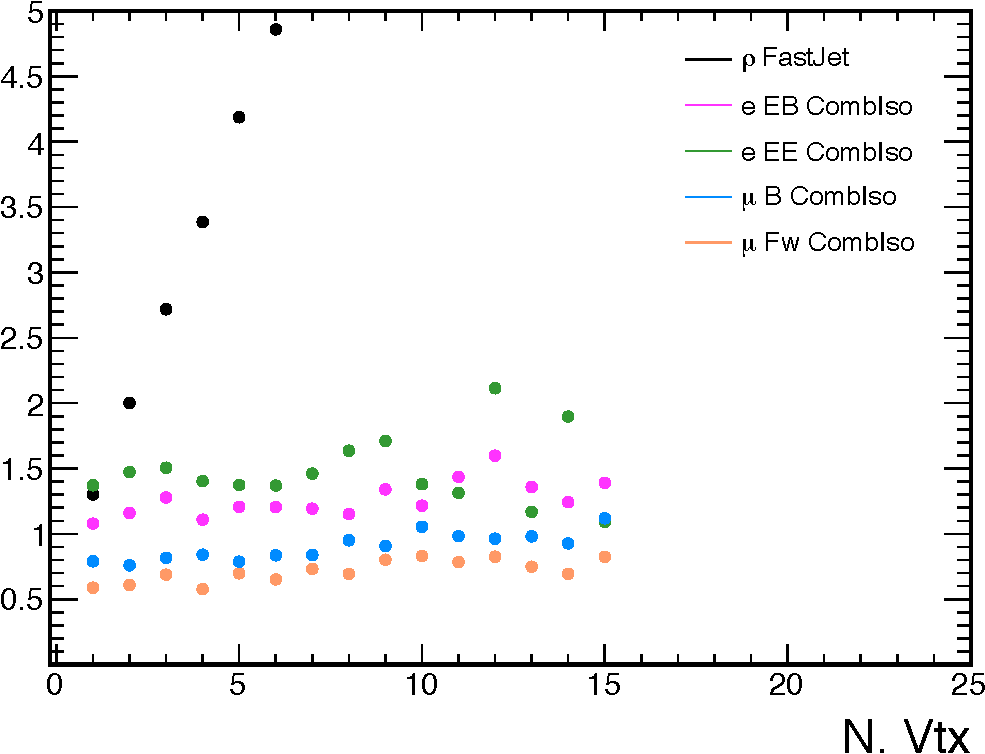
\includegraphics[width=0.47\textwidth]{figures/fastjet-after-crop}\label{fig:fastjet-after}}
  \caption[Mean values of the combined isolation sum as a function of the number of reconstructed primary vertices, before and after the pileup correction]{Mean values of the combined isolation sum as a function of the number of reconstructed primary vertices, before and after the pileup correction.  The black line is a fit to the estimated energy density due to pileup.}
  \label{fig:fastjet-correction}
\end{figure*}

The isolation sum is sensitive to pileup effects since additional interactions lead to more jet activity in the event.  To ensure a stable efficiency for the isolation requirement with respect to pileup, the isolation sum is corrected based on the \textsc{fastjet} determination of the energy density $\rho$ due to pileup and the underlying event.  The isolation sum is reduced according to the measured diffuse noise $\rho$ in the event, with effects shown in Fig.~\ref{fig:fastjet-correction}.

One final, though small, concern for electron identification comes from cases where photons are generated from internal \brem{} in $W$ and $Z$ decays, closely aligned with one of the resulting leptons.  If produced near an electron, such a photon will likely be correctly included as part of the electron's supercluster in the \ecal; if produced near a muon, however, it likely to be misidentified as a distinct electron.  To remove these ambiguities, electrons found in the immediate vicinity of a muon ($\Delta R < 0.01$) are rejected.

Detailed efficiency measurements discussed later in this chapter (see Sec.~\ref{sec:lepton-selection-efficiency}) give an overall efficiency of 73\% for an electron produced by a $W$ decay to pass our selection.  
We can investigate the misidentification rate in simulation by looking at a sample of \Zjets{} events with a \ztomumu{} decay such that all reconstructed electrons should be due to misidentified jets.  Considering all reconstructed jets and electrons with $\et > \sienergy{20}$, we find that 0.9\% of jets result in a basic electron object, with only 11\% of those passing the full $W$ decay identification and isolation criteria. 


\section{Muon Selection}
\label{sec:muon-selection}
The muon selection follows a requirement-based approach similar to that used for electrons.  Muons are restricted to be within the pseudorapidity acceptance ($|\eta| < 2.4$) of the muon and tracking systems and to fulfill various track quality requirements.  The global track fit must contain at least eleven inner tracker hits including one or more hits in the pixel detector and at least one hit in the muon system.  Moreover, the muon must be matched to track segments in two different muon stations.  In order to reject muons from hadrons decaying in flight or from kaons punching through the calorimeter, the overall quality of the global muon fit must be high as measured by a requirement on the normalized $\chi^2$ (meaning that we divide the $\chi^2$ value by the number of degrees of freedom in the fit).  To reject cosmic ray muons which do not originate from a collision, we also require that the impact parameter of the global fit with respect to the measured beam spot be less than \SI{2}{mm}.  These track quality requirements are shown in Table~\ref{tab:muon-requirements} along with the isolation values.

\begin{table*}
  \centering
  \begin{tabular}{r rrr}
    \toprule
    \multicolumn{3}{r}{Minimum number of pixel hits} & 1 \\
    \multicolumn{3}{r}{Minimum number of tracker hits} & 11 \\
    \multicolumn{3}{r}{Minimum number of muon system hits} & 1 \\
    \multicolumn{3}{r}{Minimum number of matched muon segments} & 2 \\
    \multicolumn{3}{r}{Maximum normalized $\chi^2$} & 10.0 \\
    \multicolumn{3}{r}{Maximum impact parameter (cm)} & 0.2 \\
    \midrule
    & $\mu^Z_1$ & $\mu^Z_2$ & $\mu^W$ \\ \cmidrule{2-4}
    Minimum trigger match \pt (\GeVc) & 17 & 8 & --- \\
    Minimum global track \pt (\GeVc) & 20 & 10 & 20 \\
    Maximum $R_\text{iso}$ & 0.15 & 0.15 & 0.10 \\
    \bottomrule
  \end{tabular}
  \caption[Requirements imposed on muons]{Requirements imposed on muons.  The first six rows apply to all muons considered for the analysis while the values in the final three rows take into account the specific role for which a muon has been selected.  The requirements under the headings $\mu^Z_1$ and $\mu^Z_2$ are applied to the higher-\pt and lower-\pt legs of a \ztomumu{} decay while the requirements under the heading $\mu^W$ are applied to muons assigned to a \wtomunu{} decay.}
  \label{tab:muon-requirements}
\end{table*}

\begin{figure*}[p]
  \centering
  \newcommand{\mygraph}[1]{\includegraphics[width=0.49\textwidth]{matplotlib/#1.\figext}}
  \mygraph{lepcuts100/hm_pt}\hfill\mygraph{lepcuts10/hm_iso}\\
  \mygraph{lepcuts10/hm_npix}\hfill\mygraph{lepcuts10/hm_ntrk}\\
  \mygraph{lepcuts10/hm_nmuo}\hfill\mygraph{lepcuts10/hm_nseg}\\
  \mygraph{lepcuts10/hm_chi2}\hfill\mygraph{lepcuts10/hm_d0}\\
  \caption[Distributions of criteria used to select muons]{Distributions of criteria used to select muons, considering all remaining candidates with $\pt > \simomentum{20}$ after a \ztoll{} decay is identified.  Collision data (composed mostly of jets) is compared to simulated $WZ$ events (composed mostly of true muons) to show the discriminating power of each requirement.  Shaded areas indicate excluded regions; the lighter shaded region in the $R_\text{iso}$ distribution is excluded only when considering a \wtomunu{} decay.}
  \label{muon-cuts}
\end{figure*}

Isolation for muons is exactly analogous to the algorithm for electrons (Eqs.~\ref{eq:isolation} and~\ref{eq:riso}) again with the transverse momenta and energies summed in separate $\Delta R$ cones of radius 0.3 for the tracker, \ecal, and \hcal.  Again, contributions from the muon in question are removed.  The same pileup correction is applied, depending on the number of reconstructed vertices in the event and the region of the detector in which the muon is found.

The selection used for muons is identical for those assigned to a $W$ decay vs.\ those assigned to a $Z$ decay except for a tighter isolation requirement on the $W$ and a trigger matching requirement on both muons assigned to a $Z$ decay.  As with electrons, our primary concern for muon identification is to reduce the possibility for a jet to included as a lepton in the $W$ decay where we are not protected by an invariant mass constraint.  Trigger matching and \pt cuts are exactly analogous to the electron case.

Detailed efficiency measurements discussed later in this chapter (see Sec.~\ref{sec:lepton-selection-efficiency}) give an overall efficiency of 86\% for a muon produced by a $W$ decay to pass our selection.  
We can investigate the misidentification rate in simulation by looking at a sample of \Zjets{} events with a \ztoee{} decay such that all reconstructed muons should be due to misidentified jets.  Considering all reconstructed jets with $\et > \sienergy{20}$ and all reconstructed muons with $\pt > \simomentum{20}$, we find that 0.003\% of jets result in a muon object, with only 0.6\% of those passing the full $W$ decay identification and isolation criteria.

\section{Final Selection of \textit{WZ} Candidates}
$Z$ boson candidates are built from a pair of opposite-sign, same-flavor leptons with \pt and trigger matching requirements as discussed in Secs.~\ref{sec:electron-selection} and~\ref{sec:muon-selection} along with an invariant mass between \simass{60} and \simass{120}.  If the available leptons produce more than one such combination, we choose the one most consistent with the nominal $Z$ mass.  If, however, four or more leptons are present which can yield two distinct $Z$ candidates, the event is rejected to suppress $ZZ$ background.

We assign the highest-\pt candidate from the remaining leptons to the $W$ boson decay.  The transverse mass of the $W$ boson candidate $\mt(W)$ is given as:
\begin{equation}
  \label{eq:wtransmass}
  \mt(W) \equiv \sqrt{2 \cdot \MET \cdot \pt(\ell) \cdot \Delta \phi}
\end{equation}
with $\pt(\ell)$ the transverse momentum of the lepton assigned to the $W$ and $\Delta \phi$ the angle between that lepton and the \MET in the transverse plane.  Distributions showing $M(Z)$, \MET, and $\mt(W)$ after selection of the third lepton are shown in Figs.~\ref{fig:validw-zmass}, \ref{fig:validw-met}, and~\ref{fig:validw-transmass}.  

To reject a large fraction of events without a genuine $W$ decay, we require that the \MET calculated from particle flow be above \sienergy{30}, indicating the recoil of a high-energy neutrino.

\begin{figure}
  \centering
  \includegraphics[width=\plotwidth]{matplotlib/hZMass_ValidW}
  \caption{Reconstructed mass of the $Z$ boson candidate for events with an extra isolated lepton passing requirements for the $W$.}
  \label{fig:validw-zmass}
\end{figure}

\begin{figure}
  \centering
  \includegraphics[width=\plotwidth]{matplotlib/hMET_ValidW}
  \caption{Distribution of missing transverse energy for events with a valid $Z$ candidate and an extra isolated lepton passing requirements for the $W$.}
  \label{fig:validw-met}
\end{figure}

\begin{figure}
  \centering
  \includegraphics[width=\plotwidth]{matplotlib/hWTransMass_ValidW}
  \caption{Transverse mass of the $W$ boson candidate for events with a valid $Z$ candidate and an extra isolated lepton passing requirements for the $W$.}
  \label{fig:validw-transmass}
\end{figure}

Massive exotic particles decaying via $WZ$ should be most easily distinguished from the SM $WZ$ background by virtue of a narrow width in the spectrum of the system's reconstructed mass $M(WZ)$.  That mass, however, depends on the longitudinal momentum $p_z$ of the neutrino, which cannot be inferred from the information recorded by the detector.  We proceed by assuming the $W$ to have its nominal mass, leading to a quadratic equation with $p_z(\nu)$ the only unknown.  As long as the reconstructed $\mt(W)$ lies below the nominal $W$ mass, this equation yields two real solutions.  We choose the lower magnitude of the two $p_z(\nu)$ solutions as it is found to give the $M(WZ)$ value more consistent with the generator-level $WZ$ mass in 75\% of simulated events.  Due to the finite detector resolution, some fraction of events ($\approx$ 20\%) yield a reconstructed value of $\mt(W)$ which exceeds the nominal $W$ mass and generates complex results in the $p_z(\nu)$ equation
% (see Fig.~\ref{fig:complex-angle})
.  
In these cases, we replace the $M(W)$ assumption with the measured transverse mass, recovering a unique real solution.

In addition to the invariant mass distinction, we expect that $WZ$ events originating from the decay of a massive particle should in general be more energetic than the events expected from the Standard Model.  We quantify this by considering the scalar sum of the transverse momenta of the final state leptons:
\begin{equation}
  \label{eq:lepht}
  \lepht = \sum_i \pt(\ell_i),
\end{equation}
where $i$ iterates over the three charged leptons associated with the \ztoll and \wtolnu decays.

% \begin{figure}
%   \centering
%   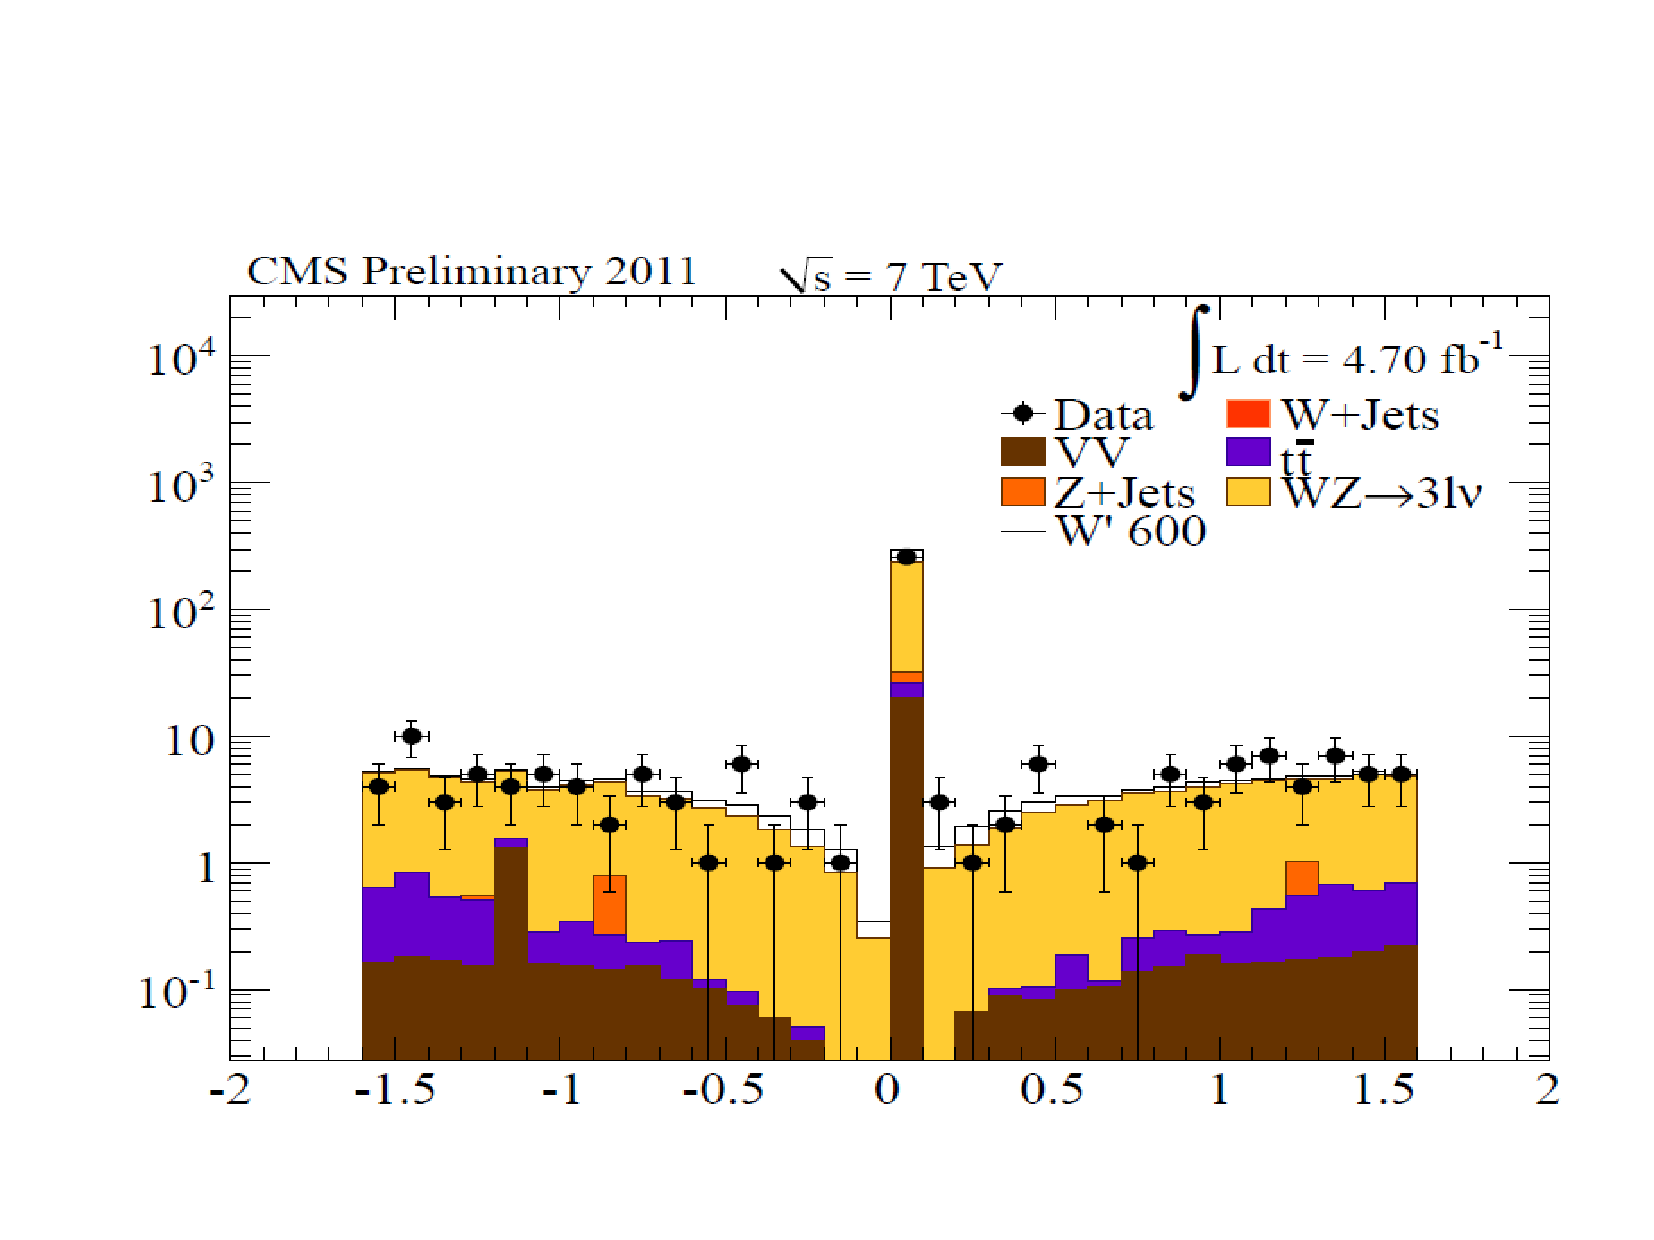
\includegraphics[width=\plotwidth]{figures/plot-complex-angle}
%   \caption{Distribution of the complex angle for the potential solutions to the quadratic equation for $p_z(\nu)$ under the nominal $M(W)$ assumption.  The large central peak corresponds to real solutions with fewer than 5\% of events having an imaginary component.}
%   \label{fig:complex-angle}
% \end{figure}

% We define the transverse mass of the $WZ$ system~\cite{Belyaev:2007ss}:
% \begin{equation}
%   \label{eq:wzmt}
%   M^2_\text{T}(WZ) = (\sqrt{M^2(\ell\ell\ell) + \pt^2(\ell\ell\ell)} + |\MET|)^2 -|\pt(\ell\ell\ell) + \MET|^2. 
% \end{equation}

We use requirements on the $M(WZ)$ and \lepht distributions to achieve further separation between resonant particles and SM $WZ$ production.  The mass windows and minimum \lepht values are determined separately for each simulated mass point, optimizing for the best expected limit.  The distributions of \lepht and invariant mass for selected $WZ$ candidates are shown in figures~\ref{fig:ht} and~\ref{fig:mwz}.

\begin{figure}
  \centering
  \includegraphics[width=\plotwidth]{matplotlib/hHt_ValidWZCand}
  \caption{Distribution of \lepht in simulated samples and collision data.}
  \label{fig:ht}
\end{figure}

\begin{figure}
  \centering
  \includegraphics[width=\plotwidth]{matplotlib/hWZMass_ValidWZCand}
  \caption{Distribution of $WZ$ invariant mass in simulated samples and collision data.}
  \label{fig:mwz}
\end{figure}

\section{Optimization of Analysis Cuts}
The selection criteria for the $W$ and $Z$ bosons, including identification and isolation of the constituent leptons, provide sufficient suppression of all background except for the genuine $WZ$ events predicted in the Standard Model.  The requirements on $M(WZ)$ and \lepht, then, are motivated by a desire to distinguish exotic particles from SM $WZ$.  Both of these requirements capitalize on the rapid suppression of the SM cross section with increasing mass beyond the threshold value of \simass{170}.  Although a mass window alone could provide significant power to discriminate against SM events, the mass resolution is poor due to its dependence on inferences about the escaping neutrino.  In comparison, the \lepht measurement plays to the strengths of the CMS detector in electron and muon reconstruction, thus providing a more reliable gauge of how energetic the system may be.  The complementary nature of these two requirements is illustrated in Fig.~\ref{fig:mass-vs-ht}.

\begin{figure}
  \centering
  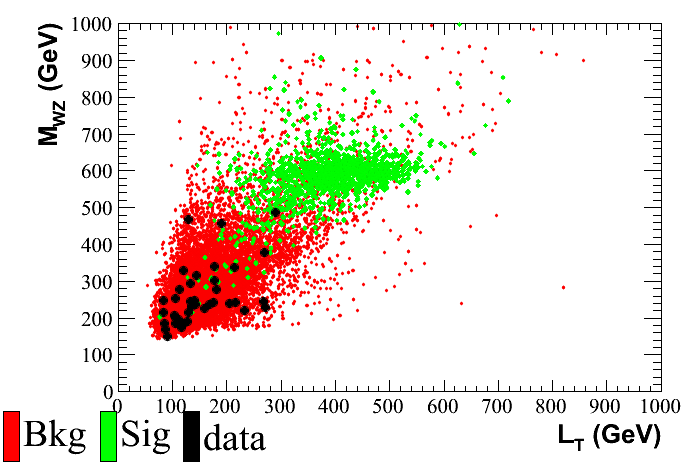
\includegraphics[width=\plotwidth]{figures/plot-mass-vs-lt.png}
  \caption[Distribution of \lepht vs. $M(WZ)$ for a \simass{600} \wprime signal sample and for $WZ$ background]{Distribution of \lepht vs. $M(WZ)$ for a \simass{600} \wprime signal sample and for $WZ$ background.  Because the samples have a significant width with respect to both parameters, substantial sensitivity gains can be achieved through a combined requirement.}
  \label{fig:mass-vs-ht}
\end{figure}

The \lepht requirements and mass windows are optimized simultaneously.  The minimum \lepht is initially set to \simomentum{50} (the minimum possible value based on the lepton \pt requirements) and increased in increments of \simomentum{10}, in line with the lepton \pt resolution.  The mass window is symmetric and centered on the nominal mass of the $WZ$ system, expanding outward in steps of \simass{10} on either side.

The requirements can be optimized with respect to various figures of merit, often some ratio between the number of signal and background events passing the selection.  We choose a full calculation of the expected limit (described in Sec.~\ref{sec:limit-technique}) for each potential mass window plus \lepht pairing as our figure of merit, choosing the combination which gives the best limit.  Due to diminishing background statistics at high $M(WZ)$, errors on the expected limit become large enough that no meaningful optimization of the \lepht requirement can be made, so we keep the requirement optimized for an \simass{800} signal when considering higher mass ranges.  The optimized requirements for each mass point are presented along with final event yields and cross section limits in Table~\ref{tab:event-yields}.  This simultaneous approach provides a marginal improvement over previous techniques which used functions of the signal and background yields to optimize the \lepht requirement and the mass window sequentially.

\section{Efficiency of Lepton Selection}
\label{sec:lepton-selection-efficiency}
We determine the efficiency of our electron and muon selection criteria by applying a ``tag and probe'' measurement to each stage of the selection.  This method exploits the $Z \to e^+ + e^-$ and $Z \to \mu^+ + \mu^-$ resonances to provide a sample of real leptons that is unbiased with respect to the quantities being measured.  The approach involves selecting events with a ``tag'' lepton passing some tight selection, then searching for a ``probe'' lepton which forms an invariant mass consistent with a $Z$ boson when paired with the tag.  Due to the mass constraint, this sample of probes can be assumed to consist almost entirely of real leptons.  If we consider our selection criteria as a series of sequential requirements, then the efficiency of a particular step is given by the fraction of probes passing all previous criteria which also pass the requirement in question.

\begin{figure*}
  \centering
  \subbottom[electrons]{\includegraphics[width=0.49\textwidth]{matplotlib/efficiencies/turnon-electron}}
  \hfill
  \subbottom[muons]{\includegraphics[width=0.49\textwidth]{matplotlib/efficiencies/turnon-muon}}
  \caption[Efficiencies for isolated electrons and muons to pass the trigger requirement as a function of \pt]{Efficiencies for well-identified, isolated (a) electrons and (b) muons (right) to pass the trigger requirement as a function of the lepton's transverse momentum.  In both cases, the trigger requires an object with $\pt > \simomentum{17}$, leading to a ``turn-on'' region with respect to the higher-resolution \pt measurement used in offline reconstruction.  The requirement that $\pt > \simomentum{20}$ on the leading reconstructed lepton assigned to the $Z$ decay is chosen to ensure all candidates are on or near the plateau of the above efficiency curves.}
  \label{fig:trigger-turnon}
\end{figure*}

These tag and probe measurements are applied to both collision data and Monte Carlo simulation in order to determine ratios which can be used to correct the event yields in simulation.  For the trigger efficiency measurements in data, special care is taken to select events from single-lepton datasets where the tag is matched to the trigger so as not to introduce a trigger bias.  For electron measurements, we use a special path designed specifically for tag and probe studies which requires a single electron object with $\et > \sienergy{17}$ along with a supercluster in the \ecal with $\et > \sienergy{8}$.  As the supercluster-finding efficiency is nearly 100\%, this requirement introduces little bias to the efficiency and identification measurements.

Results are extracted from the tag and probe samples through functional fits to the invariant mass of tag-probe pairs.  The $Z$ peak is fit with a Gaussian multiplied by an exponential to allow a low-end tail while the non-peaking background is assumed to be linear, with the resulting fit subtracted from the peak.  A systematic uncertainty is estimated for each measurement by replacing the function used to fit the $Z$ peak with other possible shapes such as a Gaussian multiplied by a quadratic.  The variation in the extracted efficiency with respect to different fitting functions is in most of these measurements less than 0.5\%.  These errors are factored into the final results as discussed in Sec.~\ref{sec:systematics}.

The observed efficiencies show various levels of dependence on the transverse momentum and pseudorapidity of the lepton.  In the trigger case, the efficiency has a sharp dependence on \pt in the immediate vicinity of the trigger threshold, but quickly reaches a plateau of near constant efficiency, as shown in Fig.~\ref{fig:trigger-turnon}.  The \pt requirements on reconstructed leptons for this analysis are chosen so as to avoid this ``turn-on'' region of the trigger efficiency curve.  For other measurements, the momentum and pseudorapidity dependence is small within the population of leptons considered in this analysis.  Because the sensitivity gains from a binned efficiency measurement would be negligible, we make a single measurement for each efficiency which represents the entire range of leptons considered.

\begin{table*}[p]
  \newcommand{\sep}{$\,\pm\,$}
  \centering
  \begin{tabular}{l l@{\sep}r l@{\sep}r l@{\sep}r}
    \toprule
    Efficiency & \multicolumn{2}{c}{Data/\%} & \multicolumn{2}{c}{MC/\%} & \multicolumn{2}{c}{Ratio ($\frac{\text{Data}}{\text{MC}}$)} \\
    \midrule
    Identification \hfill($W$) & 84.8&0.1 & 84.9&0.1 & 0.999&0.001 \\
    Isolation \hfill($W$)      & 85.6&0.1 & 81.7&0.1 & 1.047&0.002 \\
    Identification \hfill($Z$) & 97.4&0.1 & 97.6&0.1 & 0.998&0.001 \\
    Isolation \hfill($Z$)      & 97.9&0.1 & 97.3&0.1 & 1.006&0.001 \\
    Trigger \hfill($\et > \sienergy{17}$) & 95.8&0.1 & 98.2&0.1 & 0.976&0.001 \\
    Trigger \hfill($\et > \sienergy{08}$) & 95.8&0.1 & 98.2&0.1 & 0.976&0.001 \\
    \bottomrule
  \end{tabular}
  \caption[Electron efficiency values obtained from the tag and probe
fits]{Electron efficiency values obtained from the tag and probe
fits.  For each efficiency, we give the value obtained from data, the
value obtained from MC simulation, and the ratio of data to MC.  The
errors quoted are purely statistical.}
\label{tab:electron-efficiencies}
\end{table*}

\begin{figure*}[p]
  \centering
  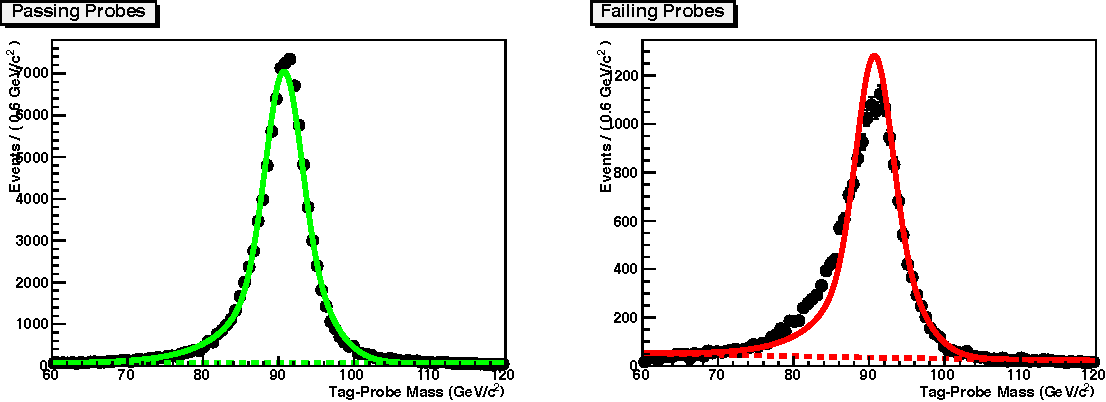
\includegraphics[width=\textwidth,clip=true]{matplotlib/efficiencies/fits-electronid-crop}
  \caption[Example fits to electron tag-probe pairs]{Fits to the invariant mass spectrum of tag-probe pairs as defined for the \wtoenu electron identification efficiency measurement.  Pairs where the probe passes the identification criteria are shown on the left while pairs where the probe fails the identification criteria are shown on the right.  In each plot, the dashed line shows the linear fit to non-peaking background while the solid line shows the fit to genuine \ztoee decays (Gaussian plus exponential).}
  \label{fig:electron-fits}
\end{figure*}

For electrons, we consider the total efficiency as the product of identification, isolation, and trigger efficiencies:
\begin{equation}
  \label{eq:factorized-eff-electron}
  \efftot = \effid \cdot \effiso \cdot \effhlt,
\end{equation}
where the efficiency for a reconstructed electron to pass identification \effid{} and the efficiency for an identified electron to pass isolation \effiso{} are calculated separately for the \ztoee and the \wtoenu selection sets while the efficiency for an isolated electron to be identified in the trigger \effhlt{} is calculated separately for each leg of the trigger since these are independent.  The reconstruction efficiency for superclusters in the \ecal{} is measured centrally to be very nearly unity in both collision data and simulation~\cite{CMS-PAS-EGM-10-004}; because the effect is negligible, we do not include it explicitly in this study.  The results of these measurements are given in Table~\ref{tab:electron-efficiencies} with examples of produced fits shown in Fig.~\ref{fig:electron-fits}.

\begin{table*}[p]
  \newcommand{\sep}{$\,\pm\,$}
  \centering
  \begin{tabular}{l l@{\sep}r l@{\sep}r l@{\sep}r}
    \toprule
    Efficiency & \multicolumn{2}{c}{Data/\%} & \multicolumn{2}{c}{MC/\%} & \multicolumn{2}{c}{Ratio ($\frac{\text{Data}}{\text{MC}}$)} \\
    \midrule
    Reconstruction (STA) & 98.4&0.1 & 98.2&0.5 & 1.002&0.005 \\
    Reconstruction (TRK) & 98.9&0.1 & 99.3&0.5 & 0.995&0.005 \\
    Identification       & 97.1&0.1 & 97.7&0.1 & 0.994&0.001 \\
    Isolation            & 95.2&0.1 & 92.5&0.2 & 1.030&0.002 \\
    Trigger \hfill($\pt > \simomentum{17}$) & 95.3&0.1 & 94.9&0.1 & 1.004&0.001 \\
    Trigger \hfill($\pt > \simomentum{08}$) & 95.3&0.1 & 94.9&0.1 & 1.004&0.001 \\
    \bottomrule
  \end{tabular}
  \caption[Muon efficiency values obtained from the tag and probe
fits]{Muon efficiency values obtained from the tag and probe
fits.  For each efficiency, we give the value obtained from data, the
value obtained from MC simulation, and the ratio of data to MC.  The
errors quoted are purely statistical.}
\label{tab:muon-efficiencies}
\end{table*}

\begin{figure*}[p]
  \centering
  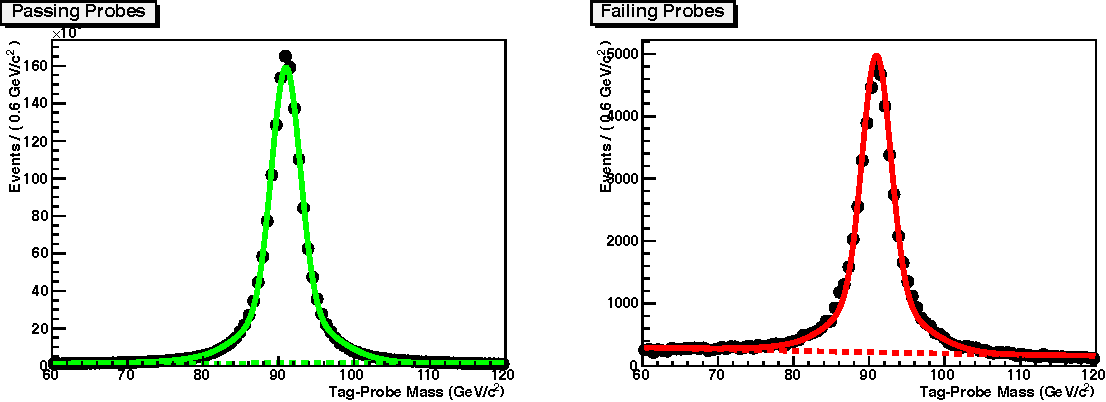
\includegraphics[width=\textwidth,clip=true]{matplotlib/efficiencies/fits-muonid-crop}
  \caption[Example fits to tag-probe muon pairs.]{Fits to the invariant mass spectrum of tag-probe pairs as defined for the muon identification efficiency measurement.  Pairs where the probe passes the identification criteria are shown on the left while pairs where the probe fails the identification criteria are shown on the right.  In each plot, the dashed line shows the linear fit to non-peaking background while the solid line shows the fit to genuine \ztomumu decays (Gaussian plus exponential).}
  \label{fig:muon-fits}
\end{figure*}

For muons, we consider the same efficiencies as above, but also \efftrk{} and \effsta{}, the efficiencies to reconstruct a track in the tracker given a stand-alone muon and to reconstruct a stand-alone muon given a track in the tracker, respectively.  The two measurements are assumed to be completely independent.  The total efficiency, then, is:
\begin{equation}
  \label{eq:factorized-eff-muon}
  \efftot = \efftrk \cdot \effsta \cdot \effid \cdot \effiso \cdot \effhlt.
\end{equation}
Results are given in Table~\ref{tab:muon-efficiencies}

We are also interested in understanding the frequency with which these electron and muon selection criteria incorrectly identify jets as leptons.  The misidentification rate is investigated in Sec.~\ref{sec:matrix-method} as part of a larger data-driven method to estimate the background contribution from \Zjets{} events.

\resetlinenumber
% \chapter{Background Studies}
\label{chapter:background}

As discussed in Sec.~\ref{sec:mc-samples}, the background processes expected to contribute to the three-lepton final state consist primarily of genuine \wtolnu{} or \ztoll{} decays along with some number of additional jets misidentified as leptons.  Because of the low probability for a jet to satisfy the lepton identification criteria, the expected contribution from a given process diminishes as the number of jets needed to fake a $WZ$ signal increases.  Accordingly, the primary concern is \Zjets{} events where only one misidentified lepton is sufficient to cause contamination, motivating a data-driven estimation method which also measures a portion of the \ttbar{} background (discussed in Sec.~\ref{sec:matrix-method}).  Other background sources are estimated from MC simulation where possible with agreement between the collision data and simulation evaluated in various ``control regions'' (Sec.~\ref{sec:control-regions}).  For the resonance search, all backgrounds are taken from simulation, considering samples representing diboson processes with extra jets ($WW$, $WZ$, $ZZ$, $Z\gamma$, and $W\gamma$) along with \Zjets, \Wjets, and \ttbar.  For the $WZ$ cross section measurement, only $ZZ$ and $Z\gamma$ are taken from simulation; data-driven methods are used directly to account for all other background contributions.

\section{\emph{Z} + jets Background Estimation}
\label{sec:matrix-method}

When possible, it is advantageous to reduce a measurement's reliance on the quality of MC simulation by performing investigations directly in the collision data.  In particular, we would like to define a method to extract an estimate of the yield of dominant background processes in our final signal sample which can then be used to replace or verify the Monte Carlo results.
To that end, we use the ``matrix method''~\cite{CMS-PAS-EWK-11-010} to perform a data-driven estimation of the contribution to the signal region from backgrounds where a misidentified jet accompanies a $Z$ candidate formed from real leptons; this will be primarily composed of \Zjets{} events, although there may also be small contributions from \ttbar{} and $WW$ processes.  The resulting estimates are used directly in the cross section measurement discussed in Chapter~\ref{chapter:cross-section} and indirectly as a check on the simulated yields for the resonance search in Chapter~\ref{chapter:limits}.

The matrix method seeks to compare the number \nlep of $WZ$ candidate events where the $W$ decay has been associated with a genuine electron or muon to the number \njet of events where the lepton candidate for the $W$ decay is in fact a misidentified jet.  These numbers, of course, are not directly observable in collision data, so we instead count the number \ntight of events passing all selection criteria for $W$ and $Z$ candidates and compare this to the superset of events \nloose obtained by removing the isolation requirement on the lepton candidate assigned to the $W$ decay.  By carefully measuring the efficiency \etight of the isolation criteria for real leptons and the corresponding efficiency (or, from another perspective, ``fake rate'') \pfake for misidentified jets, we obtain a system of equations which allow us to obtain values for \nlep{} and \njet:
\begin{align}
  \nloose &= \nlep + \njet \\
  \ntight &= \etight\cdot\nlep + \pfake\cdot\njet.
\end{align}

\begin{table}
  \centering
  \newcommand{\ph}{}
  \begin{tabular}{l r@{$\,\pm\,$}l}
    \toprule
    Measurement & \multicolumn{2}{c}{Efficiency/\%} \\
    \midrule
    $\etight(e)$   & 93.59 & 0.04 \\
    $\etight(\mu)$ & 97.11 & 0.02 \\
    $\pfake(e)$    &  7\ph & 1\ph \\
    $\pfake(\mu)$  &  6\ph & 1\ph \\
    \bottomrule
  \end{tabular}
  \caption{Measured isolation efficiencies for genuine leptons and misidentified jets.}
  \label{tab:efficiencies}
\end{table}

We apply the tag and probe method in independent samples of collision data as described below to determine the \etight{} and \pfake{} values for electrons and muons given in Table~\ref{tab:efficiencies}.  The final background estimate is determined separately for each mass window, with the data-driven results compared to generator-level information in MC samples in Table~\ref{tab:matrix-results}.

\begin{table}
  \centering 
  \begin{tabular}{ c r@{$\pm$}l r@{$\pm$}l r@{$\pm$}l }
    \toprule
    $M(\wprime)c^2/\GeV$ & \multicolumn{2}{c}{$\etight\cdot\nlep$} & \multicolumn{2}{c}{$\pfake\cdot\njet$} & \multicolumn{2}{c}{$N_\text{lep}^\text{MC}$} \\
    \midrule
    \phantom{0}200 & \phantom{00}46 & 7 & 6.4 & 0.9 & 41 & 6 \\
    \phantom{0}250 & 36 & 6 & 3.7 & 0.6 &  27 & 5 \\
    \phantom{0}300 & 19 & 5 & 3.6 & 0.6 &  19 & 4 \\
    \phantom{0}400 & 6 & 3 & 1.2 & 0.3 &  11 & 3 \\
    \phantom{0}500 & 8 & 3 & 0.6 & 0.2 &  6 & 3 \\
    \phantom{0}600 & 2 & 1 & 0.1 & 0.1 & 3 & 2 \\
    \phantom{0}700 & 2 & 1 & 0.1 & 0.1 & 2 & 1 \\
    \phantom{0}800 & 1 & 1 & 0.1 & 0.1 & 0.9 & 0.9 \\
    \phantom{0}900 & 0 & 0 & 0 & 0 & 0.9 & 0.9 \\
              1000 & 0 & 0 & 0 & 0 &  0.7 & 0.8 \\
              1100 & 0 & 0 & 0 & 0 &  0.5 & 0.7 \\
              1200 & 0 & 0 & 0 & 0 &  0.4 & 0.6 \\
              1300 & 0 & 0 & 0 & 0 &  0.3 & 0.5 \\
              1400 & 0 & 0 & 0 & 0 &  0.2 & 0.4 \\
              1500 & 0 & 0 & 0 & 0 & 0.1 & 0.3 \\
    \bottomrule
  \end{tabular}
  \caption[Results of the matrix method for background estimation]{Expected numbers of selected events with the $W$ decay assigned to either a genuine lepton or a misidentified jet.  The measured number of true leptons $\etight\cdot\nlep$ may be compared with the expected number of signal-like events with isolated leptons based on Monte Carlo information in the final column.}
  \label{tab:matrix-results}
\end{table}

\subsection{Measurement of Isolation Efficiency for Genuine Leptons}
For the \etight{} measurement, we want to define some collection of lepton candidates that has a high purity of genuine leptons, but without using any isolation criterion that would bias our measurement.  This is accomplished through the same tag and probe method employed in the measurement of lepton selection efficiencies in Sec.~\ref{sec:lepton-selection-efficiency}.  We define a $Z$-enriched region in the collision data by selecting events with exactly one pair of same-flavor, opposite-charge leptons with $\pt > \simomentum{10}$ and invariant mass between \simass{60} and \simass{120}.  Both leptons must pass the identification criteria imposed on candidates for the $W$ decay and at least one must pass the associated isolation requirement, serving as the tag object.  The remaining lepton candidate serves as the probe.

The resulting dataset is dominated by \Zjets, but also includes some \ttbar, $WZ$, and \Wjets events.  The processes with a genuine \ztoll{} decay contribute to a peak in the invariant mass distribution while the \ttbar and \Wjets contributions tend to be evenly distributed across the invariant mass range.  To obtain a best estimate of the number of genuine \ztoll{} events within the sample, we make a linear fit to the sidebands ([70,80] and [100,110] \GeVcc) of the invariant mass distribution and use this to subtract the non-peaking events.

The value of \etight{} is obtained by counting the total number of events with the probe passing isolation $N_\text{pass}$ and the total number of events with the probe failing isolation $N_\text{fail}$, subtracting the estimated contributions to each of these distributions from the linear fits $B_\text{pass}$ and $B_\text{fail}$, and taking the ratio of passing events to total events:
\begin{equation}
  \etight = \frac{2(N_\text{pass} - B_\text{pass})}{(N_\text{fail} - B_\text{fail}) + 2(N_\text{pass} - B_\text{pass})}.
\end{equation}

\subsection{Measurement of Isolation Efficiency for Misidentified Jets}
To measure \pfake{}, we need to define some collection of lepton candidates which we believe with a high confidence to be from jets, but without using any isolation criterion which would bias the measurement.  Because the interaction topologies are very similar for the production of charged and neutral vector bosons at the LHC, we expect a similar spectrum of jets in events with a $W$ when compared to events with a $Z$.  As a result, we can perform the \pfake{} measurement on a $W$-enriched sample in the collision data where we have eliminated \ztoll{} decays.  In order to define a region dominated by \Wjets, we select events with a lepton (serving as tag) which meets the identification and isolation criteria imposed on candidates for the $W$ decay along with $\MET > \simass{20}$, $\mt(W) > \simass{20}$, and exactly one additional lepton candidate with opposite flavor (since $Z$ decays can never give one electron and one muon) which passes the identification criteria without isolation.  The value of \pfake{} is given simply as the ratio of the event count with the probe passing isolation to the total number of selected events in the $W$-enriched region.

\section{QCD Background Estimation}

Any analysis performed with CMS must also consider possible contamination from raw multijet events due to the high LHC cross section for pure QCD processes.  Within the context of this analysis, significant contamination from QCD would be highly unlikely due to the nature of the selection criteria.  Most multijet events come from soft interactions which generate little transverse momentum such that the lepton \pt requirements alone significantly reduce the relevant QCD cross section.  Beyond this, the $Z$ mass window and requirement of significant \MET{} provide tight constraints on the kinematics of the event which pure multijet interactions are unlikely to replicate.

The potential of our kinematic selection to suppress QCD is well demonstrated by the \Wjets{} background.  Containing a real \wtolnu{} decay, this process should have a similar \MET distribution to genuine $WZ$ events, so all of our discriminating power comes from the $Z$ mass constraint along with lepton selection requirements sufficient to avoid misidentification of two jets as leptons.  Although \Wjets{} has the highest cross section among MC background samples considered in this analysis, its contribution in the final sample is negligible.  While the cross section for events with three or more jets dwarfs that for \Wjets{} events by approximately four orders of magnitude~\cite{LopezMateos}, the low probability for multijet events to produce substantial \MET while also overcoming lepton selection requirements on an additional jet compensates for the high event rate.

Verifying the above arguments through a direct MC investigation of the expected QCD contribution is not feasible due to the extremely large statistics of simulated QCD data which would be necessary for any reasonable estimation.  An early study of the CMS detector's sensitivity to Technicolor signatures~\cite{CMS-PAS-EXO-09-007}, however, utilized a limited sample of QCD events to measure individual probabilities that a multijet event would yield a $Z$ candidate, a $W$ candidate, or high \lepht.  Treating the probabilities to find a $Z$ or a $W$ as independent and employing selection criteria very similar to that presented here, they conservatively estimate a contribution of less than \SI{0.5}{events/\fbinv} passing all selection criteria in the lowest-mass search windows, a level corresponding to less than 10\% of the total yield from other background processes.

\section{Control Regions}
\label{sec:control-regions}

The event selection criteria presented in the previous sections of this chapter are each motivated by physical arguments about the differences between signal and background.  As such, the quality of the selection is dependent upon the validity and scope of those arguments, so it is essential to consider some set of orthogonal data regions or tangential event characteristics in order to evaluate whether the selection is comprehensive and well understood.  These investigations are taken as ``controls'' on the selection criteria, verifying that the characteristics of the collision data are sufficiently well-modeled by simulation that the selection criteria can be trusted.

{\newcommand{\myplot}[1]{\includegraphics[width=0.49\textwidth]{matplotlib/analysis/#1}}

\begin{figure*}
  \centering
  \myplot{hZMass_ValidZ}\hfill\myplot{hZMass_ValidWZCand}\\
  \caption[Invariant mass distribution of reconstructed $Z$ candidates for two selections]{Invariant mass distribution for reconstructed $Z$ candidates before a $W$ candidate is selected (left) and after $W$ selection and \MET requirements are applied (right).}
  \label{fig:control-zmass}
\end{figure*}

\begin{figure*}
  \centering
  \myplot{hZpt_ValidZ}\hfill\myplot{hZpt_ValidWZCand}\\
  \caption[Transverse momentum distribution of reconstructed $Z$ candidates for two selections]{Transverse momentum distribution of selected $Z$ candidates before a $W$ candidate is selected (left) and after $W$ selection and \MET requirements are applied (right).}
  \label{fig:control-zpt}
\end{figure*}

\begin{figure*}
  \centering
  \myplot{hNJets_ValidZ}\hfill\myplot{hNJets_ValidWZCand}\\
  \caption[Jet multiplicity distribution for two selections]{Jet multiplicity distribution before a $W$ candidate is selected (left) and after $W$ selection and \MET requirements are applied (right).}
  \label{fig:control-njets}
\end{figure*}

\begin{figure*}
  \centering
  \myplot{jetPtFirst_COMB}\hfill\myplot{jetPtSecond_COMB}\\
  \caption[Transverse energy distributions of leading and next-to-leading jets]{Transverse energy distributions of leading (left) and next-to-leading (right) jets before a $W$ candidate is selected.}
  \label{fig:control-jetet}
\end{figure*}
}

Before initial selection of a third lepton to associate with the $W$ decay, the selected data will be composed primarily of events with a real $Z$ boson that may be accompanied by one or more jets.  In this ``pre-$W$'' region, we are first concerned about validating the quality of our $Z$ boson reconstruction as demonstrated by the invariant mass and transverse momentum distributions shown in Figs.~\ref{fig:control-zmass} and~\ref{fig:control-zpt}.  We are also interested in evaluating the quality of jet modeling in this region, since the upcoming $W$ selection criteria are designed primarily to avoid misidentification of a jet as a lepton resulting from a $W$ decay.  The jet multiplicity is given in Fig.~\ref{fig:control-njets} along with the transverse energies of the leading and next-to-leading jets in Fig.~\ref{fig:control-jetet}.

{\newcommand{\myplot}[1]{\includegraphics[width=0.49\textwidth]{matplotlib/analysis/#1}}

\begin{figure*}
  \centering
  \myplot{hWTransMass_ValidW}\hfill\myplot{hWTransMass_ValidWZCand}\\
  \caption[$W$ transverse mass distribution for two selections]{Transverse mass of the selected $W$ candidate before the \MET requirement is applied (left) and after (right).}
  \label{fig:control-wtransmass}
\end{figure*}

\begin{figure*}
  \centering
  \myplot{hHT_3e}\hfill
  \myplot{hHT_2e}\\
  \myplot{hHT_2mu}\hfill
  \myplot{hHT_3mu}\\
  \caption{Distribution of \lepht{} after the \MET requirement is applied, shown separately for each of the four decay channels.}
  \label{fig:control-lepht}
\end{figure*}

\begin{figure*}
  \centering
  \myplot{hWZ3e0muMass_ValidWZCand}\hfill
  \myplot{hWZ2e1muMass_ValidWZCand}\\
  \myplot{hWZ1e2muMass_ValidWZCand}\hfill
  \myplot{hWZ0e3muMass_ValidWZCand}\\
  \caption{Mass of the $WZ$ candidate after the \MET requirement is applied, shown separately for each of the four decay channels.}
  \label{fig:control-wzmass}
\end{figure*}

} % End \myplot region.

After the selection of an isolated lepton for the \wtolnu decay, our primary concern becomes the quality of $W$ candidate modeling and reconstruction.  The distribution of missing transverse energy associated with the escaping neutrino has already been shown in Fig.~\ref{fig:validw-met}, but we now add Fig.~\ref{fig:control-wtransmass} which shows the $W$ boson's transverse mass (as defined in Eq.~\ref{eq:wtransmass}).

After imposing the requirement for significant \MET, the data sample should be dominated by direct SM $WZ$ events with only small contributions from other massive diboson processes.  This ``full $WZ$ selection'' region allows validation of the $WZ$ pair production background before application of analysis-level selection aimed at enhancing sensitivity to a possible massive resonance.  The \lepht{} and $WZ$ invariant mass distributions in this region have been previously presented in Figs.~\ref{fig:ht} and~\ref{fig:mwz}.  As the identification criteria and efficiencies are substantially different for electrons vs.\ muons, however, we also break these distributions down by decay channel in Figs.~\ref{fig:control-lepht} and~\ref{fig:control-wzmass}.

In all cases, the agreement between data and simulation indicates a sufficient understanding of the selected region to lend confidence to our measurements of the $WZ$ system.

% In our case, we evaluate several tangential distributions at various points along the chain of selection criteria.  Figs.~\ref{fig:control-zmass}--\ref{fig:control-njets} show distributions of the $Z$ mass, $Z$ transverse momentum, and jet multiplicity both at the point of the initial $Z$ selection and after the $W$ selection and \MET requirements have been applied.  Fig.~\ref{fig:control-wtransmass} shows the $W$ transverse mass distribution both at the point of the initial $W$ selection and after the \MET requirement has been applied.  Fig.~\ref{fig:control-wzmass} shows the mass of the $WZ$ candidate separately in each of the four channels.  The agreement between data and simulation indicates a good understanding of the selected data region.
\resetlinenumber
% \chapter{Cross Section Measurement}
\label{chapter:cross-section}

\newcommand{\nsig}{\ensuremath{N_\mathrm{sig}}\xspace}
\newcommand{\nbkg}{\ensuremath{N_\mathrm{bkg}}\xspace}
\newcommand{\nobs}{\ensuremath{N_\mathrm{obs}}\xspace}
\newcommand{\esim}{\ensuremath{\epsilon_\mathrm{sim}}\xspace}
\newcommand{\errmat}{\textbf{\textit{E}}\xspace}

The latest CMS measurement of the $WZ$ cross section was performed in the summer of 2011 with a dataset corresponding to \earlylumi~\cite{CMS-PAS-EWK-11-010}.  This chapter gives a summary of that effort.  Although much of the analysis approach is identical to the resonance measurement, this early study did not have access to the same range of updated tools and MC samples that were available for work on the full 2011 dataset, so some differences will be discussed.

\section{Technique for Measuring a Cross Section}

The $WZ$ cross section measurement is based on the formula:
\begin{equation}
  \label{eq:simple-cross-section}
  \sigma = \frac{N_\text{signal}}{A\cdot\epsilon\cdot\mathcal{L}},
\end{equation}
with number of observed signal events \nsig, fiducial and kinematic acceptance $A$, selection efficiency $\epsilon$ for events in acceptance, and integrated luminosity $\mathcal{L}$.  The value of $A$ is affected by the choice of PDF and other theoretical uncertainties, while the value of  $\epsilon$ is susceptible to errors from triggering and reconstruction.  In order to control the efficiency uncertainties, we concentrate on the extraction of corrections to the efficiencies obtained from the simulation. These correction factors come from efficiency
ratios $\rho = \epsilon / \esim$ derived by measuring $\epsilon$ and $\esim$ in the same way on data and simulation, respectively. We then replace the product $A \cdot \epsilon$ by the product $\mathcal{F} \cdot \rho$ with $\mathcal{F} \equiv  A \cdot \esim$ the fraction of generated $WZ$ events with dilepton mass between \simass{60} and \simass{120} selected in the simulation.  Furthermore, the number of signal events \nsig{} is not measured directly but is obtained by subtracting the estimated number of background events \nbkg{} from the observed number of selected candidate $WZ$ events \nobs.

Equation~\ref{eq:simple-cross-section} can therefore be rewritten as
\begin{equation}
\sigma = (1-f_{\tau})\frac{\nobs-\nbkg}{\mathcal{F} \cdot \rho \cdot \mathcal{L}},
\label{eq:x-sectionDef2}
\end{equation}
with $f_{\tau}$ the fraction of reconstructed $WZ$ events containing a tau lepton as determined from simulation.  For \nbkg, we use yields estimated from both MC simulation and data-driven methods:
\begin{equation}
  \nbkg = \pfake \cdot \njet + N_\text{MC}^{ZZ} + N_\text{MC}^{Z\gamma},
\end{equation}
where $\pfake \cdot \njet$ gives the matrix method estimate (Sec.~\ref{sec:matrix-method}) for backgrounds containing a real lepton pair accompanied by a misidentified jet (dominated by \Zjets events, but also accounting for \ttbar and $WW$ contributions, values given in Table~\ref{tab:xsec-matrix-results}) while the minor $ZZ$ and $Z\gamma$ yields are taken directly from simulated samples.

\begin{table}
  \newcommand{\sep}{$\,\pm\,$}
  \centering
  \begin{tabular}{c l@{\sep}r l@{\sep}r l@{\sep}r}
    \toprule
    Channel & \multicolumn{2}{c}{$\etight \cdot \nlep$} & \multicolumn{2}{c}{$\pfake\cdot\njet$} & \multicolumn{2}{c}{$N_\text{lepton}^\text{tight}$} \\
    \midrule
    ${e}{e}{e}$ & 20.24&4.76 & 1.76&0.67 & 14.47&3.80\\
    ${e}{e}\mu$ & 17.46&4.56 & 2.54&0.86 & 17.49&4.18\\
    $\mu\mu{e}$ & 11.40&3.67 & 1.60&0.58 & 13.95&3.73\\
    $\mu\mu\mu$ & 17.82&4.54 & 2.18&0.76 & 18.56&4.31\\
  \bottomrule
  \end{tabular}
  \caption[Results of the matrix method for background estimation]{Expected numbers of background events from \Zjets{} and \ttbar{} as determined by the matrix method on the first \earlylumi{} of 2011 $pp$ collision data.  The measured number of true leptons $\etight \cdot \nlep$ may be compared with the expected number of tight leptons from signal-like events based on MC simulation information $N_\text{lepton}^\text{tight}$.}
  \label{tab:xsec-matrix-results}
\end{table}

\begin{table*}
  \newcommand{\sep}{$\,\pm\,$}
  \centering
  \newcommand{\mubox}[1]{\makebox[\widthof{$\mu$}][c]{$#1$}}
  \newcommand{\chbox}[3]{\ensuremath{\mubox{$#1$}^+ \mubox{$#2$}^- \mubox{$#3$}^\pm}}
  \begin{tabular}{c l@{\sep}r l@{\sep}r l@{\sep}r c r@{\sep}r@{\sep}r@{\sep}r}
    \toprule
    Channel & \multicolumn{2}{c}{$A$/\%} & \multicolumn{2}{c}{$\mathcal{F}$/\%} & \multicolumn{2}{c}{$\rho$} & \nobs & \multicolumn{4}{c}{$(\sigma\times\text{BR})$/fb} \\
    \midrule
    \chbox{$  e$}{$  e$}{$  e$} & 48.2&0.3 & 19.3&0.3 & 0.97&0.07 & 22 & 86&22&8&5\\
    \chbox{$  e$}{$  e$}{$\mu$}   & 48.8&0.3 & 23.4&0.3 & 1.00&0.06 & 20 & 60&17&5&4\\
    \chbox{$\mu$}{$\mu$}{$  e$} & 43.2&0.3 & 19.0&0.3 & 0.94&0.04 & 13 & 53&18&4&3\\
    \chbox{$\mu$}{$\mu$}{$\mu$} & 45.4&0.3 & 24.9&0.3 & 0.97&0.04 & 20 & 60&16&4&4\\
  \bottomrule
  \end{tabular}
  \caption[Measured cross sections by channel]{Acceptance, efficiency, simulation correction factor, number of observed events, and calculated cross section for each of the four decay channels.  The cross section are given as central values followed by statistical, systematic, and luminosity uncertainties.}
  \label{tab:channel-breakdown}
\end{table*}

We determine the cross section $\sigma(pp \to W + Z \to \ell + \nu_\ell + \ell^{\prime +} + \ell^{\prime -})$ by first performing separate measurements for each of the four channels ($eee$, $ee\mu$, $\mu\mu e$, $\mu\mu\mu$) and later combining them for a final result.  The results for each channel are given in Table~\ref{tab:channel-breakdown}.

\section{Common Systematic Uncertainties}
\label{sec:systematics}

The $WZ$ cross section measurement and the resonance search rely largely on the same set of analysis tools, thus the methods for estimating systematic uncertainties on these two measurements are largely the same.  The relative effect, however, of the various contributions can differ considerably in the two analyses.  Chapters~\ref{chapter:cross-section} and~\ref{chapter:limits} detail the specific impact of each component on the relevant result.

We consider the systematic uncertainties which contribute to the limit results in three distinct categories.  The first group concerns sources of uncertainty on the product of acceptance, reconstruction, and identification efficiencies for final-state objects.  This includes both uncertainties in the detector performance and in the theoretical models used to generate the Monte Carlo samples.

To estimate the detector uncertainties in this first group, we study the event yields for simulated samples of signal and background under variation of each parameter of interest.  For \MET, we consider variations on the resolution and the energy scale, defining windows of possible values by comparing performance between data and MC.  For leptons, we consider 1\% variations on the muon momentum scale and 2\% variations on the electron energy scale.  Finally, we consider variations on the vertex multiplicity distribution to account for mismeasurement of pileup.  All simulated events are weighted based on the number of reconstructed vertices in order to match the distribution for collision events with an assumed minimum bias cross section of \SI{73.5}{mb}.  To estimate the uncertainty on this reweighting process, we shift by $\pm 1$ vertex the Poisson mean of the vertex multiplicity distribution measured in data.  On the theoretical side, this first group includes uncertainties due to the choice of parton distribution functions (PDFs).  The \textsc{cteq6}~\cite{Pumplin:2002vw} PDF set was used with uncertainties determined according to the method described in Ref.~\cite{Campbell:2006wx}.

The second group concerns uncertainties on the data \vs{} simulation correction factors for the efficiencies of the trigger, reconstruction, and identification requirements.  As described in Sec.~\ref{sec:lepton-selection-efficiency}, the efficiencies are determined using a tag and probe method in both simulation and collision data, with the ratio of the efficiencies used to scale simulated events.  The uncertainty on these efficiencies is estimated by varying the fitting function used in the efficiency determination, with the error propagated to the resulting ratio.

The third group concerns theoretical uncertainties on the background yields.  For the resonance search, the first major contribution comes from uncertainties in the NLO $k$-factor (Sec.~\ref{sec:mc-samples}) corrections for $WZ$.  As the \MADGRAPH{} sample used for simulating the $WZ$ process contains explicit production of additional jets at the matrix element level, it is expected to give a reasonably correct kinematical description of the higher-order contributions, allowing us to apply a simple scale factor to the entire sample in order to match the total NLO cross section computed with MCFM.  A comparison of several kinematic distributions between the LO \MADGRAPH sample and events from MCFM shows agreement in all cases within 10\%, which we take as the uncertainty on the $k$-factors.  Where relevant, cross-section uncertainties of 7.5\% for $ZZ$~\cite{Campbell:2011bn}, 13\% for $Z\gamma$~\cite{VGammaCMS}, and 17\% for $WZ$~\cite{CMS-PAS-EWK-11-010} are also considered along with an uncertainty on the integrated luminosity~\cite{LUMIPAS}.

\section{Systematic Errors for the Cross Section Measurement}

As discussed in Sec.~\ref{sec:systematics}, systematic uncertainties fall generally into three groups.  In the case of this cross section measurement, the uncertainties from the first group affect the calculated value of $\mathcal{F}$ while the uncertainties from the second group affect the correction factor $\rho$ and uncertainties from the third group affect the $WZ$ yield.  All values given in Table~\ref{tab:xsec-systematics}.  These calculations are performed using the early 2011 dataset and its associated calibrations.  As a result, some of these errors are larger than those considered in the resonance search.

\begin{table}
  \centering
  \begin{tabular}{l cccc}
    \toprule
    Effect on $\mathcal{F}$ (\%)  & ${e}{e}{e}$ & ${e}{e}\mu$ & $\mu\mu{e}$ & $\mu\mu\mu$ \\
    \midrule
    Electron energy scale         & 1.7 & 0.3 & 0.9 & --- \\
    Muon $p_T$ scale              & --- & 0.5 & 0.2 & 0.9 \\ 
    \MET Resolution                & 0.5 & 0.5 & 0.5 & 0.5 \\
    \MET Scale                     & 0.3 & 0.2 & 0.1 & 0.1 \\
    Pileup                        & 3.1 & 0.8 & 1.6 & 1.6 \\
    PDF                           & 1.0 & 1.0 & 1.0 & 1.0 \\ 
    NLO effect                    & 2.5 & 2.5 & 2.5 & 2.5 \\ \addlinespace[0.5em]
    Total                         & 4.5 & 2.9 & 3.3 & 3.3 \\
    \midrule\midrule
    Effect on $\rho$ (\%)         & ${e}{e}{e}$ & ${e}{e}\mu$ & $\mu\mu{e}$ & $\mu\mu\mu$ \\ 
    \midrule
    Electron trigger		  & 1.5 & 1.5 & --- & --- \\ 
    Electron reconstruction       & 2.7 & 1.8 & 0.9 & --- \\ 
    Electron ID and isolation     & 5.9 & 5.0 & 3.2 & --- \\
    Muon trigger                  & --- & --- & 1.1 & 1.1 \\
    Muon reconstruction           & --- & 0.7 & 1.5 & 2.2 \\ 
    Muon ID and isolation         & --- & 0.7 & 1.5 & 1.9 \\ \addlinespace[0.5em]
    Total                         & 6.7 & 5.6 & 4.2 & 3.6 \\ 
    \midrule\midrule
    Effect on $WZ$ Yield (\%)     & ${e}{e}{e}$ & ${e}{e}\mu$ & $\mu\mu{e}$ & $\mu\mu\mu$ \\ 
    \midrule
    $\sigma(ZZ)$                  & 0.2 & 0.4 & 0.3 & 0.4 \\
    $\sigma(Z\gamma)$             & 0.5 & 0.1 & 0.1 & 0.1 \\
    $\sigma(\ttbar)$              & 1.3 & 1.3 & 0.9 & 0.5 \\
    $P_\text{fake}$                & 3.3 & 4.9 & 5.2 & 4.2 \\
    \bottomrule
    \end{tabular}
    \caption[Summary of systematic uncertainties on the cross section measurements in each of the four channels]{Summary of systematic uncertainties on the cross section measurements in each of the four channels.  A uniform uncertainty of 6\% on the integrated luminosity is also considered in all channels.}
    \label{tab:xsec-systematics}
\end{table}

\section{Cross Section Combination}

The final cross section estimation, taking into account the correlation between systematic uncertainties for the different channels, is performed using the Best Linear Unbiased Estimator (BLUE)~\cite{Lyons:1988rp}.  The combined cross section is taken to be a linear combination of the measured cross sections in each of the four channels:
\begin{equation}
  \sigma(\wztolnll) = \sum_i^4 \alpha_i\cdot\sigma_i
\end{equation}
with $\sigma_i$ the per-channel cross sections and weighting factors $\alpha_i$ determined by minimizing the variance subject to the constraint:
\begin{equation}
  \sum_i^4 \alpha_i = 1.
\end{equation}

The variance $\sigma^2$ (with $\sigma$ used here as the standard symbol for error rather than cross section) can be expressed as:
\begin{equation}
  \sigma^2 = \tilde{\alpha} \, \errmat \, \alpha,
\end{equation}
with \errmat the error matrix, $\alpha$ a vector composed of the weighting factors $\alpha_i$, and $\tilde{\alpha}$ its transpose.  By applying the method of Lagrangian multipliers, we obtain:
\begin{equation}
  \alpha = \frac{\errmat^{-1} U}{\tilde{U}\,\errmat^{-1}U},
\end{equation}
with $U$ a vector whose four components are all unity and $\errmat^{-1}$ the inverse of the error matrix.

\newcommand{\scorr}{\sigma^\text{corr}}
\newcommand{\discorr}[2]{\scorr_{#1#2}\scorr_{#2#1}}

The error matrix itself is given as:
\begin{equation}
  \errmat = \left(
    \begin{array}{cccc}
      \sigma_1^2     & \discorr{1}{2} & \discorr{1}{3} & \discorr{1}{4} \\
      \discorr{2}{1} & \sigma_2^2     & \discorr{2}{3} & \discorr{2}{4} \\
      \discorr{3}{1} & \discorr{3}{2} & \sigma_3^2     & \discorr{3}{4} \\
      \discorr{4}{1} & \discorr{4}{2} & \discorr{4}{3} & \sigma_4^2     \\
 \end{array}
\right),
\end{equation}
with $\sigma_i^2$ the variances on the $WZ$ cross section measurements in each channel and $\scorr_{ij}$ the correlated components of the uncertainties on those measurements for the combination.

The calculated value of the error matrix, taking into account statistical and systematic uncertainties along with correlations in the systematics is:
\begin{equation}
 \errmat = \left(
 \begin{array}{cccc}
 5.25  & 0.26  & 0.27 & 0.07  \\
 0.26  & 3.00  & 0.10 & 0.13  \\
 0.27  & 0.10  & 3.25 & 0.06  \\
 0.07  & 0.13  & 0.06 & 2.76  \\
 \end{array}
\right) \times \SI{e-4}{\pb^2},
\end{equation}
leading to weighting factors $\alpha = (0.15, 0.28, 0.26, 0.32)$ and a final combined cross section for $\simass{60} < M(Z) < \simass{120}$ over the full acceptance:
\begin{align}
  \sigma(pp \to &W + Z \to \ell + \nu_\ell + \ell^{\prime +} + \ell^{\prime -}) = \notag\\
  & 0.062 \pm 0.009 (\text{stat.}) \pm 0.004 (\text{syst.}) \pm 0.004 (\text{lumi.}) \pb,
\end{align}
which, taking into account the measured values of the leptonic branching ratios of the $W$ and $Z$~\cite{Nakamura:2010zzi}, corresponds to an inclusive cross section:
\begin{align}
  \sigma(p + p \to &W + Z) = \notag\\
  & 17.0 \pm 2.4 (\text{stat.}) \pm 1.1 (\text{syst.}) \pm 1.0 (\text{lumi.}) \pb.
\end{align}
Within error, the result shows good agreement with the NLO theoretical prediction (Eq.~\ref{eq:predicted-cross-section}) over the same phase space:
\begin{align}
  \sigma(p + p \to &W + Z) = \notag\\
  & 18.57 \pm 0.95\,\si{pb}.
\end{align}

\chapter{Limits on New Resonances}
\label{chapter:limits}

\section{Statistical Technique for Setting a Limit}
\label{sec:limit-technique}

We calculate exclusion limits on the production cross section $\sigma(p + p \to \wprime/\technirho \to W^\pm + Z) \times \text{BR}(\wztolnll)$ by comparing the numbers of observed events with the numbers of expected signal and background events from Monte Carlo simulation.  Before counting events in the MC samples, we apply a scale factor to each event based on the data vs.\ MC ratios obtained for the electron and muon efficiencies; the value of the scale factor is chosen based on the decay channels of the reconstructed $W$ and $Z$.

In order to evaluate a limit on the cross section for a particular mass hypothesis, we must define some test statistic which depends on the signal rate $\mu$.  A good preliminary choice would be a profile likelihood ratio $p_\mu$, but this statistic is prone to overestimation of the excluded region due to small statistical fluctuations in regions where sensitivity is low~\cite{Nakamura:2010zzi}.  To address this issue, we replace $p_\mu$ with the modified statistic:
\begin{equation}
  \confcls{} = \frac{p_\mu}{1 - p_{0}},
\end{equation}
with $p_0$ the $p$-value of the background-only hypothesis.

The number of background events contributing to the signal region is not expected to match exactly with the results of the background estimation technique.  Rather, we would expect repetitions of the experiment to yield varying numbers of background events distributed around the background estimation value as a mean.  To account for this effect, we model the background as a Poisson probability density function and perform many background-only \emph{pseudoexperiments} in which Monte Carlo techniques are used to sample the model distribution.

The expected limit must also take into account any significant ``nuisance parameters'', measured quantities which affect the model, but which are of no interest in the final result.  The two nuisance parameters identified for our study are the measured luminosity and the product of detector acceptance and efficiency.  We model each of these as with a Gaussian distribution using the measured value as the mean and the associated systematic uncertainty as the width.  

In practice, we use the \texttt{CL95} implementation of \confcls{} statistics in the \texttt{RooStats}~\cite{roostats} package to calculate 95\% confidence level exclusions defined by regions where the \confcls{} statistic falls below 5\%.  Expected limits are taken as the median value derived from 1000 MC pseudoexperiments in which random seeds are used to sample values from each of the background yield, luminosity, and efficiency distributions.

\section{Systematic Errors}

As discussed in Sec.~\ref{sec:systematics}, systematic uncertainties fall generally into three groups.  The first group consists of effects which can alter the yield of observed events, with results of studies in simulation for signal and background given in Table~\ref{tab:scale-systematics} for detector effects and~\ref{tab:pdf-systematics} for the choice of PDF.  Events with higher values for $M(WZ)$ correspond to collisions with higher energy $\hat{s}$ in the parton center of momentum frame and are sensitive to momentum fractions for which the PDF uncertainty is larger.  In particular, the PDF uncertainties for the $q\bar{q}$ and $gg$ processes become significantly larger for large values of $\hat{s}/s$.  This effect, mixed with the lower statistics available for high-mass $WZ$, leads to significantly larger errors on the $WZ$ background simulation for higher-mass search windows.

\begin{table*}
  \newcommand{\myS}{\ensuremath{\frac{\sigma_S}{S}}}
  \newcommand{\myB}{\ensuremath{\frac{\sigma_B}{B}}}
  \newcommand{\compressedslash}{\hspace{-.10em}/\hspace{-.08em}}
  \newcommand{\mypair}{\myB\compressedslash\% & \myS\compressedslash\%}
  \newcommand{\mymass}[1]{\makebox[\widthof{0000}][r]{#1}}
  \centering
  \begin{tabular}{c ll ll ll ll ll}
    \toprule
    %\multirow{2}{*}{$\displaystyle\frac{M(\wprime)}{\GeVcc}$} 
    & \multicolumn{2}{c}{\MET Scale} & \multicolumn{2}{c}{$\sigma(\MET)$} & \multicolumn{2}{c}{Pileup} & \multicolumn{2}{c}{$\pt(\mu)$ Scale} & \multicolumn{2}{c}{$\et(e)$ Scale} \\
    \cmidrule(r){2-3} \cmidrule(rl){4-5} \cmidrule(rl){6-7} \cmidrule(rl){8-9} \cmidrule(l){10-11}
    $M(\!\wprime)$\hspace{-0.5em} & \mypair & \mypair & \mypair & \mypair & \mypair \\
    \midrule
    \mymass{ 200} & 0.99 & 0.01 & 0.52 & 1.9   & 1.7   & 0.31 & 0.45 & 3.1   & 1.0  & 1.9 \\
    \mymass{ 250} & 0.24 & 0.90 & 0.59 & 1.3   & 2.2   & 0.58 & 2.5  & 1.6   & 3.1  & 2.5 \\
    \mymass{ 300} & 1.1  & 0.49 & 0.72 & 0.97  & 1.9   & 2.0  & 2.2  & 0.51  & 4.3  & 1.3 \\
    \mymass{ 400} & 1.7  & 0.43 & 0.77 & 0.53  & 2.2   & 0.71 & 1.9  & 1.0   & 4.2  & 2.2 \\
    \mymass{ 500} & 1.8  & 0.38 & 0.91 & 0.36  & 2.6   & 2.3  & 1.7  & 0.71  & 3.6  & 1.5 \\
    \mymass{ 600} & 1.3  & 0.10 & 1.4  & 0.30  & 1.7   & 1.6  & 3.1  & 0.55  & 4.8  & 1.6 \\
    \mymass{ 700} & 2.4  & 0.15 & 1.7  & 0.23  & 3.0   & 0.82 & 5.3  & 0.91  & 4.2  & 1.7 \\
    \mymass{ 800} & 3.9  & 0.28 & 1.9  & 0.20  & 4.0   & 1.4  & 3.9  & 0.87  & 4.3  & 1.7 \\
    \mymass{ 900} & 2.3  & 0.24 & 1.9  & 0.13  & 3.6   & 1.6  & 3.0  & 0.72  & 6.4  & 0.94\\
    \mymass{1000} & 2.7  & 0.03 & 2.4  & 0.12  & 0.36  & 1.4  & 5.0  & 0.37  & 8.7  & 0.49\\
    \mymass{1100} & 1.1  & 0.16 & 2.2  & 0.13  & 0.83  & 1.1  & 2.6  & 0.15  & 6.7  & 0.51\\
    \mymass{1200} & 0.16 & 0.13 & 2.6  & 0.12  & 1.3   & 1.2  & 2.8  & 0.34  & 13   & 0.54\\
    \mymass{1300} & 0.70 & 0.10 & 2.9  & 0.12  & 1.3   & 1.9  & 4.7  & 0.12  & 5.7  & 0.38\\
    \mymass{1400} & 4.7  & 0.10 & 3.7  & 0.14  & 2.3   & 1.4  & 4.2  & 0.46  & 8.2  & 0.85\\
    \mymass{1500} & 0.01 & 0.02 & 4.2  & 0.19  & 0.92  & 2.6  & 0.72 & 0.37  & 11   & 1.3 \\
    \bottomrule
  \end{tabular}
  \caption[Summary of systematic uncertainties]{Summary of systematic uncertainties associated with \MET scale, \MET resolution, pileup, muon momentum scale, and electron energy scale.  Values show the maximum expected percent variation in Monte Carlo event yields for the sum of background samples (\myB) and for the \wprime signal (\myS).}
  \label{tab:scale-systematics}
\end{table*}

\begin{table}
  \compressedtext
  \centering
  \newcommand{\mymass}[1]{\makebox[\widthof{0000}][r]{#1}}
  \begin{tabular}{crr}
    \toprule
    & \multicolumn{2}{c}{$\sigma(\text{PDF})$/\%} \\ \cmidrule{2-3}
    $M(\wprime)c^2/\GeV$ & \wprime & $WZ$ \\
    \midrule
    \mymass{ 200} & 2.370 &  3.2 \\
    \mymass{ 250} & 2.370 &  3.4 \\
    \mymass{ 300} & 2.370 &  3.3 \\
    \mymass{ 400} & 2.764 &  3.2 \\
    \mymass{ 500} & 3.181 &  3.6 \\
    \mymass{ 600} & 3.704 &  4.0 \\
    \mymass{ 700} & 4.198 &  4.7 \\
    \mymass{ 800} & 4.624 &  4.8 \\
    \mymass{ 900} & 5.135 &  6.3 \\
    \mymass{1000} & 5.695 &  8.9 \\
    \mymass{1100} & 6.088 &  7.8 \\
    \mymass{1200} & 6.516 & 12\phantom{.0} \\
    \mymass{1300} & 7.349 & 28\phantom{.0} \\
    \mymass{1400} & 7.760 &  7.8 \\
    \mymass{1500} & 8.471 &  0.0 \\
    \bottomrule
  \end{tabular}
  \caption[PDF uncertainties for the final event selection for Monte Carlo samples]{PDF uncertainties for the final event selection for Monte Carlo samples, both \wprime{} signal and SM $WZ$ background.  Because no values were published for \wprime masses less than \simass{300}, the first two samples are assumed to have the same uncertainty as the \simass{300} case.}
  \label{tab:pdf-systematics}
\end{table}

The data \vs{} simulation correction factors and associated uncertainties are those determined previously in Sec.~\ref{sec:lepton-selection-efficiency} with the ratio values and uncertainties given in Table~\ref{tab:electron-efficiencies} for electrons and Table~\ref{tab:muon-efficiencies} for muons.  We also consider the $WZ$, $ZZ$, and $Z\gamma$ cross section uncertainties as discussed in Sec.~\ref{sec:systematics} and a 2.2\% uncertainty on the luminosity.

\section{Limit Results}

\begin{table*}
  \compressedtext
  \newcommand{\ph}{\phantom{0}}
  \newcommand{\phh}{\phantom{}}
  \newcommand{\mymass}[1]{\makebox[\widthof{0000}][r]{#1}}
  \centering
  \begin{tabular}{c r r r r@{$\,\pm\,$}l r@{$\,\pm\,$}l r@{$\,\pm\,$}l l l}
    \toprule
    & \multicolumn{2}{c}{Selection} & \multicolumn{7}{c}{Event Yields} & \multicolumn{2}{c}{Limit/pb} \\
    \cmidrule(lr){2-3} \cmidrule(lr){4-10} \cmidrule(l){11-12}
    $M(\wprime)$ & $\lepht^\text{min}$ & $w_M$ & $N_\text{data}$ & 
    \multicolumn{2}{c}{$N_\text{MC}^\text{background}$} & 
    \multicolumn{2}{c}{$N_\text{MC}^\text{signal}$} & 
    \multicolumn{2}{c}{$\epsilon_\text{MC}^\text{signal}$/\%} & 
    $\sigma^\text{upper}_\text{exp}$ & $\sigma^\text{upper}_\text{obs}$ \\
    \midrule         
    \mymass{ 200} & --- &  20 & 52 & 47.3\ph&0.7 & 300\phh&10  &  8.0&0.4 & 0.064  & 0.072  \\
    \mymass{ 250} & 150 &  40 & 40 & 32.2\ph&0.9 & 280\phh&10  &  8.8&0.4 & 0.043  & 0.061  \\ 
    \mymass{ 300} & 160 &  40 & 23 & 22.9\ph&0.7 & 330\phh&10  &   18&1   & 0.017  & 0.017  \\ 
    \mymass{ 400} & 220 &  80 &  7 & 12.0\ph&0.2 & 167\phh& 4  &   29&1   & 0.0066 & 0.0047 \\ 
    \mymass{ 500} & 230 & 100 &  9 &  8.0\ph&1.0 &  91\phh& 2  &   41&1   & 0.0037 & 0.0047 \\ 
    \mymass{ 600} & 290 & 120 &  2 &  3.2\ph&0.1 & 45.9\ph&0.8 &   45&1   & 0.0022 & 0.0020 \\ 
    \mymass{ 700} & 360 & 160 &  2 & 1.69&0.09 & 24.4\ph&0.4 &   48&1   & 0.0018 & 0.0021 \\ 
    \mymass{ 800} & 400 & 180 &  1 & 0.96&0.07 & 14.5\ph&0.2 &   52&2   & 0.0013 & 0.0015 \\ 
    \mymass{ 900} & 400 & 280 &  0 & 0.97&0.07 & 9.5\ph&0.2  &   61&2   & 0.0012 & 0.0010 \\ 
    \mymass{1000} & 400 & 360 &  0 & 0.72&0.06 & 5.97&0.09   &   65&2   & 0.0011 & 0.0010 \\ 
    \mymass{1100} & 400 & 420 &  0 & 0.52&0.05 & 3.57&0.06   &   63&1   & 0.0010 & 0.0010 \\ 
    \mymass{1200} & 400 & 520 &  0 & 0.39&0.04 & 2.04&0.03   &   58&1   & 0.0011 & 0.0011 \\
    \mymass{1300} & 400 & 560 &  0 & 0.32&0.04 & 1.12&0.02   &   50&1   & 0.0013 & 0.0012 \\
    \mymass{1400} & 400 & 580 &  0 & 0.17&0.03 & 0.52&0.01   &   36&1   & 0.0017 & 0.0017 \\
    \mymass{1500} & 400 & 600 &  0 & 0.12&0.02 & 0.28&0.01 &   30&1   & 0.0021 & 0.0020 \\
    \bottomrule
  \end{tabular}
  \caption[Values for the optimized requirements and cross section limits]{For each mass point (in \GeVcc): values of the minimum \lepht{} requirement (in \GeVc); full width of the search window centered on the targeted mass (in \GeVcc); number of events selected in data; numbers of events selected in simulated samples for sum of backgrounds and for signal; the efficiency of the full selection as measured in signal MC; and the expected and observed 95\% \conflevel{} upper limits on the cross section for a new physics signal.}
  \label{tab:event-yields}
\end{table*}

The final results of the measurement, shown in Table~\ref{tab:event-yields}, can be interpreted in various models.
In the Sequential Standard Model, the calculated cross section limits exclude \wprime bosons with masses below \wprimelimit{} (Fig.~\ref{fig:limit-vs-mass}).  In the reference Technicolor parameter space ($M(\technipi)=\frac{3}{4}M(\technirho) - \simass{25}$), they exclude $\technirho$ hadrons with masses between \tclimitlhlower{} and  \tclimitlh{} (Fig.~\ref{fig:limit-vs-mass}). We also set limits for Technicolor as a function of the $\technirho$ and $\technipi$ masses (Fig.~\ref{fig:tclimit-2d}). For the parameter space chosen by the \dzero{} experiment ($M(\technirho) < M(\technipi) + M(W)$), we obtain improved limits excluding the $M(\technirho)$ range from \tclimitdzerolower{} to \tclimitdzero{}.

\begin{figure}
  \centering
  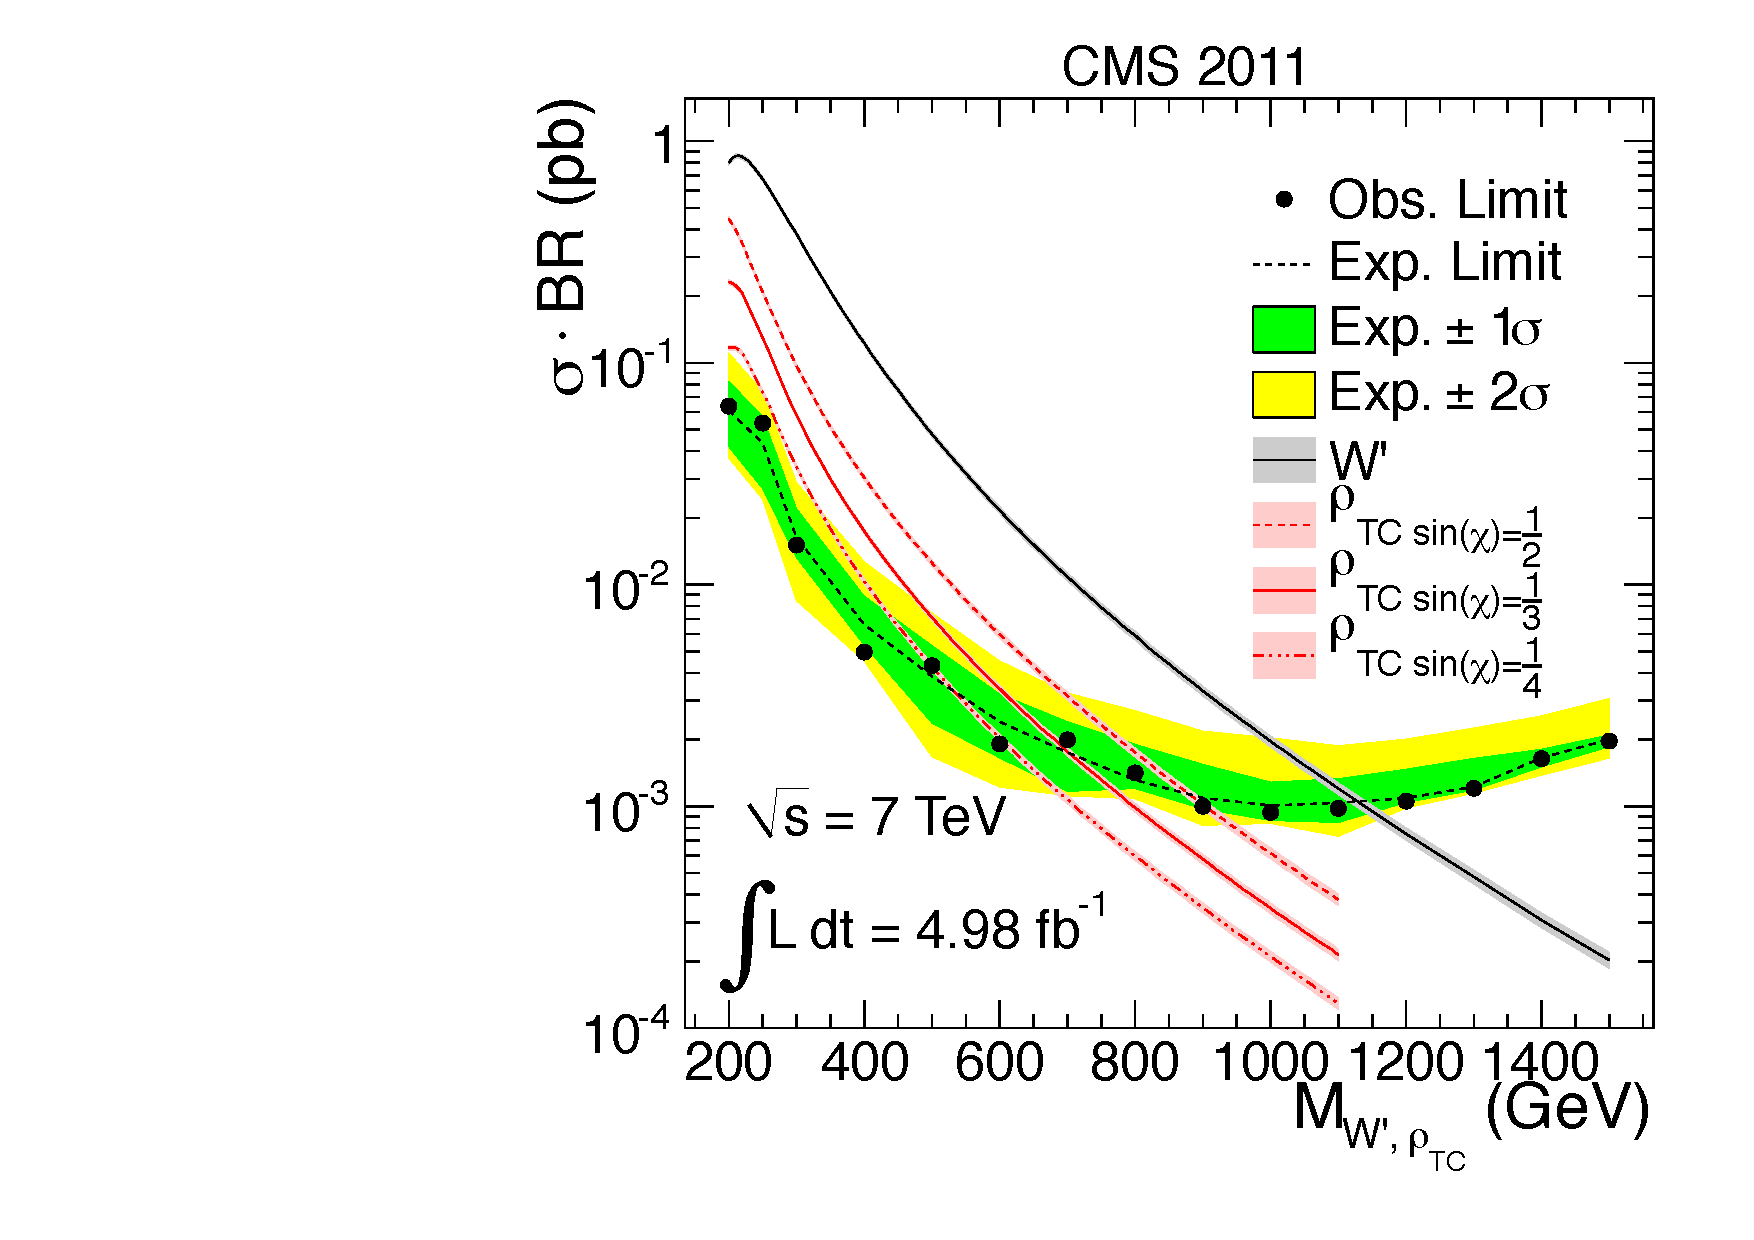
\includegraphics[width=\plotwidth]{figures/limit-vs-mass}
  \caption[Expected and observed upper limits on cross sections as a function of resonance mass]{Expected and observed 95\% C.L.\ upper limits on cross sections as a function of resonance mass for \wprime and \technirho along with the combined statistical and systematic uncertainties depicted with dark green (\SI{1}{$\sigma$}) and light yellow (\SI{2}{$\sigma$}) bands.  The theoretical cross sections (with bands showing the associated PDF uncertainty) include a mass-dependent NNLO $k$-factor.}
  \label{fig:limit-vs-mass}
\end{figure}

It has recently been suggested~\cite{Eichten:2012br} that investigations into Low-Scale Technicolor should evaluate the cross section for $\technirho \to W + Z$ as a function of the model parameter $\sin(\chi)$ since its value has a significant impact on the branching ratios for $\technirho \to W + Z$ and $\technirho \to W + \technipi$, among others.  We take $\sin(\chi) = \frac{1}{3}$ as our nominal value for limit calculations, but additional bands for $\sin(\chi) = \frac{1}{2}$ and $\sin(\chi) = \frac{1}{4}$ are shown in Fig.~\ref{fig:limit-vs-mass}.

\begin{figure}
  \centering
  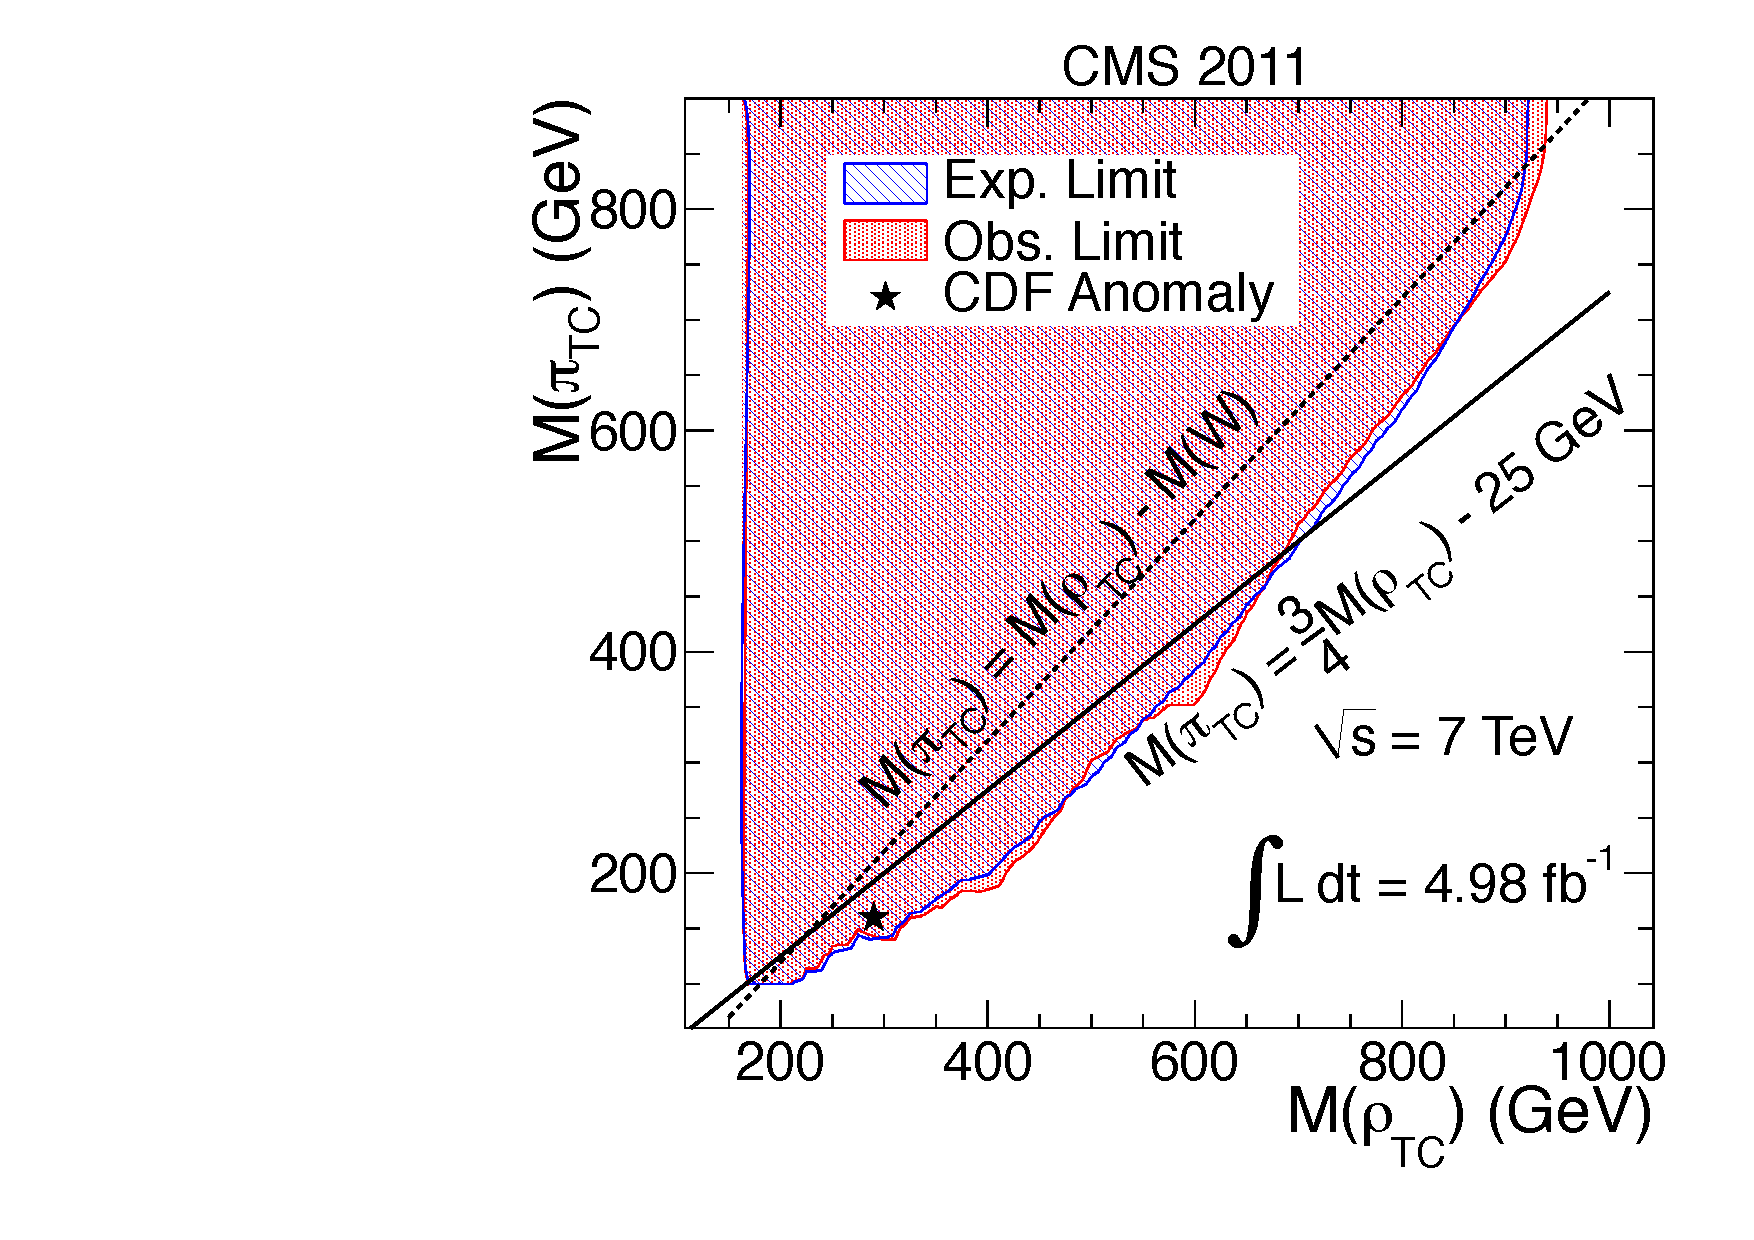
\includegraphics[width=\plotwidth]{figures/tclimit-2d}
  \caption{Exclusion limits for Low-Scale Technicolor as a function of the \technirho and \technipi masses.  The proposed Technicolor interpretation of the CDF anomaly lies inside the excluded region.}
  \label{fig:tclimit-2d}
\end{figure}

One final configuration of interest for Technicolor is motivated by the observation of an excess in the invariant mass spectrum for pairs of jets produced in association with a $W$ boson by the CDF experiment~\cite{Aaltonen:2011mk}.  Many sources have offered interpretations of this ``CDF anomaly'' in terms of new physics models, including a Technicolor configuration with tightly constrained masses for the \technirho (\simass{290}) and \technipi (\simass{160})~\cite{Eichten:2012br}.  For this particular value of $M(\technirho)$, our results place a 95\% \conflevel{} upper bound of \simass{150} for the \technipi mass, barely excluding the Technicolor interpretation.
\resetlinenumber
% \chapter{Conclusion}

\section{Summary}

A complete analysis of associated $WZ$ production with leptonic decays from proton-proton collisions is presented.  All investigations consider \SI{7}{\TeV} collisions produced at the LHC in 2011 recorded with the CMS detector.  Final state particles are reconstructed through software algorithms to select collision events with three well-identified, high-momentum, isolated leptons along with substantial \MET.

The $WZ$ production cross section is measured using a subset of the 2011 collision data corresponding to an integrated luminosity of \earlylumi.  A selected sample of 75 $WZ$ candidate events is compared to simulation of background events, taking into consideration the acceptance and efficiency for identifying signal events as determined from simulation.  Cross sections are determined individually for each of the four leptonic decay channels with the final result taken as the best fit linear combination, giving $\sigma(W + Z \to \ell + \nu_\ell + \ell^{\prime +} + \ell^{\prime -}) = 0.062 \pm 0.009 (\text{stat.}) \pm 0.004 (\text{syst.}) \pm 0.004 (\text{lumi.}) \pb$.

A resonance search in the $WZ$ invariant mass spectrum is performed using the full 2011 $pp$ dataset, corresponding to an integrated luminosity of \jsonlumi.  Several new particle mass hypotheses are considered, with analysis criteria optimized for each hypothesis, allowing calculation of 95\% confidence level upper limits on the cross section for a new particle in each mass window.  The cross section limits are interpreted in the Sequential Standard Model to rule out a \wprime{} with mass below \simass{1141} and in various configurations of Technicolor parameter space, greatly extending the \technirho exclusion region and disfavoring the Technicolor interpretation of CDF's dijet mass anomaly.

\section{Outlook}

Although the 2011 LHC dataset has already allowed us to reach beyond the limits set by the Tevatron on new physics in the $WZ$ channel, the results presented here are still dominated by statistical errors.  The upgrades currently in operation for the 2012 runs have driven up the center of mass collision energy by 14\% to \SI{8}{\TeV} and nearly achieved the LHC design luminosity.  The expected 2012 collision yield is four times that of the 2011 dataset, giving increased statistics for substantially more precise cross-section measurements.  The reach for a resonant search will be significantly extended by both the additional statistics and the increased collision energy.
\resetlinenumber

% \bibliographystyle{utcaps}
% \bibliography{klukas-thesis}

\end{document}
